%  LaTeX support: latex@mdpi.com 
%  In case you need support, please attach all files that are necessary for compiling as well as the log file, and specify the details of your LaTeX setup (which operating system and LaTeX version / tools you are using).

%=================================================================
\documentclass[sensors,review,accept,moreauthors,pdftex]{Definitions/mdpi} 

% If you would like to post an early version of this manuscript as a preprint, you may use preprint as the journal and change 'submit' to 'accept'. The document class line would be, e.g., \documentclass[preprints,article,accept,moreauthors,pdftex]{mdpi}. This is especially recommended for submission to arXiv, where line numbers should be removed before posting. For preprints.org, the editorial staff will make this change immediately prior to posting.
\setitemize{parsep=6pt,itemsep=0pt,leftmargin=*,labelsep=5.5mm}
\setenumerate{parsep=6pt,itemsep=0pt,leftmargin=*,labelsep=5.5mm}
\setlist[description]{itemsep=0mm}  
%--------------------
% Class Options:
%--------------------
%----------
% journal
%----------
% Choose between the following MDPI journals:
% acoustics, actuators, addictions, admsci, aerospace, agriculture, agriengineering, agronomy, algorithms, animals, antibiotics, antibodies, antioxidants, applsci, arts, asc, asi, atmosphere, atoms, axioms, batteries, bdcc, behavsci , beverages, bioengineering, biology, biomedicines, biomimetics, biomolecules, biosensors, brainsci , buildings, cancers, carbon , catalysts, cells, ceramics, challenges, chemengineering, chemistry, chemosensors, children, cleantechnol, climate, clockssleep, cmd, coatings, colloids, computation, computers, condensedmatter, cosmetics, cryptography, crystals, dairy, data, dentistry, designs , diagnostics, diseases, diversity, drones, econometrics, economies, education, ejihpe, electrochem, electronics, energies, entropy, environments, epigenomes, est, fermentation, fibers, fire, fishes, fluids, foods, forecasting, forests, fractalfract, futureinternet, futurephys, galaxies, games, gastrointestdisord, gels, genealogy, genes, geohazards, geosciences, geriatrics, hazardousmatters, healthcare, heritage, highthroughput, horticulturae, humanities, hydrology, ijerph, ijfs, ijgi, ijms, ijns, ijtpp, informatics, information, infrastructures, inorganics, insects, instruments, inventions, iot, j, jcdd, jcm, jcp, jcs, jdb, jfb, jfmk, jimaging, jintelligence, jlpea, jmmp, jmse, jnt, jof, joitmc, jpm, jrfm, jsan, land, languages, laws, life, literature, logistics, lubricants, machines, magnetochemistry, make, marinedrugs, materials, mathematics, mca, medicina, medicines, medsci, membranes, metabolites, metals, microarrays, micromachines, microorganisms, minerals, modelling, molbank, molecules, mps, mti, nanomaterials, ncrna, neuroglia, nitrogen, notspecified, nutrients, ohbm, optics, particles, pathogens, pharmaceuticals, pharmaceutics, pharmacy, philosophies, photonics, physics, plants, plasma, polymers, polysaccharides, preprints , proceedings, processes, proteomes, psych, publications, quantumrep, quaternary, qubs, reactions, recycling, religions, remotesensing, reports, resources, risks, robotics, safety, sci, scipharm, sensors, separations, sexes, signals, sinusitis, smartcities, sna, societies, socsci, soilsystems, sports, standards, stats, surfaces, surgeries, sustainability, symmetry, systems, technologies, test, toxics, toxins, tropicalmed, universe, urbansci, vaccines, vehicles, vetsci, vibration, viruses, vision, water, wem, wevj

%---------
% article
%---------
% The default type of manuscript is "article", but can be replaced by: 
% abstract, addendum, article, benchmark, book, bookreview, briefreport, casereport, changes, comment, commentary, communication, conceptpaper, conferenceproceedings, correction, conferencereport, expressionofconcern, extendedabstract, meetingreport, creative, datadescriptor, discussion, editorial, essay, erratum, hypothesis, interestingimages, letter, meetingreport, newbookreceived, obituary, opinion, projectreport, reply, retraction, review, perspective, protocol, shortnote, supfile, technicalnote, viewpoint
% supfile = supplementary materials

%----------
% submit
%----------
% The class option "submit" will be changed to "accept" by the Editorial Office when the paper is accepted. This will only make changes to the frontpage (e.g., the logo of the journal will get visible), the headings, and the copyright information. Also, line numbering will be removed. Journal info and pagination for accepted papers will also be assigned by the Editorial Office.

%------------------
% moreauthors
%------------------
% If there is only one author the class option oneauthor should be used. Otherwise use the class option moreauthors.

%---------
% pdftex
%---------
% The option pdftex is for use with pdfLaTeX. If eps figures are used, remove the option pdftex and use LaTeX and dvi2pdf.

%=================================================================
\firstpage{1} 
\makeatletter 
\setcounter{page}{\@firstpage} 
\makeatother
\pubvolume{xx}
\issuenum{1}
\articlenumber{5}
\pubyear{2020}
\copyrightyear{2020}
%\externaleditor{Academic Editor: name}
\history{Received: 30 November 2019; Accepted: 25 February 2020; Published: 27 April 2020}
%\updates{yes} % If there is an update available, un-comment this line

%% MDPI internal command: uncomment if new journal that already uses continuous page numbers 
%\continuouspages{yes}

%------------------------------------------------------------------
% The following line should be uncommented if the LaTeX file is uploaded to arXiv.org
%\pdfoutput=1

%=================================================================
% Add packages and commands here. The following packages are loaded in our class file: fontenc, calc, indentfirst, fancyhdr, graphicx, lastpage, ifthen, lineno, float, amsmath, setspace, enumitem, mathpazo, booktabs, titlesec, etoolbox, amsthm, hyphenat, natbib, hyperref, footmisc, geometry, caption, url, mdframed, tabto, soul, multirow, microtype, tikz
\makeatletter
\newcommand\newtag[2]{#1\def\@currentlabel{#1}\label{#2}}
\makeatother
\usepackage{longtable}
\usepackage{multirow}
%=================================================================
%% Please use the following mathematics environments: Theorem, Lemma, Corollary, Proposition, Characterization, Property, Problem, Example, ExamplesandDefinitions, Hypothesis, Remark, Definition, Notation, Assumption
%% For proofs, please use the proof environment (the amsthm package is loaded by the MDPI class).

%=================================================================
% Full title of the paper (Capitalized)
\Title{Real-Time Hand Gesture Recognition Using Surface Electromyography and Machine Learning: A~Systematic Literature Review}

% Author Orchid ID: enter ID or remove command
\newcommand{\orcidauthorA}{0000-0001-7434-4533} % Add \orcidA{} behind the author's name
\newcommand{\orcidauthorB}{0000-0002-5275-7262} % Add \orcidB{} behind the author's name
\newcommand{\orcidauthorC}{0000-0003-1723-1916}

% Authors, for the paper (add full first names)
\Author{Andr\'es Jaramillo-Y\'anez $^{1,2,}$*\orcidA{}, Marco E. Benalc\'azar $^{1}$\orcidB{} and Elisa Mena-Maldonado $^{1}$\orcidC{}}

% Authors, for metadata in PDF
\AuthorNames{Andr\'es Jaramillo-Y\'anez, Marco E. Benalc\'azar and Elisa Mena-Maldonado}

% Affiliations / Addresses (Add [1] after \address if there is only one affiliation.)
\address{%
$^{1}$ \quad Artificial Intelligence and Computer Vision Research Lab, Department of Informatics and Computer Science, Escuela Polit\'ecnica Nacional, Quito 170517, Ecuador; marco.benalcazar@epn.edu.ec (M.E.B.); elisa.k.mena@gmail.com (E.M.-M.)\\
$^{2}$ \quad School of Science, Royal Melbourne Institute of Technology (RMIT), Melbourne 3000, Australia; andres.jaramillo.yanez@rmit.edu.au (A.J.-Y.)}

% Contact information of the corresponding author
\corres{Correspondence: andres.jaramilloy@epn.edu.ec}

% Current address and/or shared authorship
%\firstnote{Current address: Affiliation 3} 
%\secondnote{These authors contributed equally to this work.}
% The commands \thirdnote{} till \eighthnote{} are available for further notes

%\simplesumm{} % Simple summary

%\conference{} % An extended version of a conference paper

% Abstract (Do not insert blank lines, i.e. \\) 
\abstract{Today, daily life is composed of many computing systems, therefore interacting with them in a natural way makes the communication process more comfortable. Human--Computer Interaction (HCI) has been developed to overcome the communication barriers between humans and computers. One form of HCI is Hand Gesture Recognition (HGR), which predicts the class and the instant of execution of a given movement of the hand. One possible input for these models is surface electromyography (EMG), which records the electrical activity of skeletal muscles. EMG signals contain information about the intention of movement generated by the human brain. This systematic literature review analyses the state-of-the-art of real-time hand gesture recognition models using EMG data and machine learning. We selected and assessed 65 primary studies following the Kitchenham methodology. Based on a common structure of machine learning-based systems, we analyzed the structure of the proposed models and standardized concepts in regard to the types of models, data acquisition, segmentation, preprocessing, feature extraction, classification, postprocessing, real-time processing, types of gestures, and evaluation metrics. Finally, we also identified trends and gaps that could open new directions of work for future research in the area of gesture recognition using EMG.}

% Keywords
\keyword{ human--computer interaction; hand gesture recognition; systematic literature review; machine learning; electromyography; real-time systems}

% The fields PACS, MSC, and JEL may be left empty or commented out if not applicable
%\PACS{J0101}
%\MSC{}
%\JEL{}

%%%%%%%%%%%%%%%%%%%%%%%%%%%%%%%%%%%%%%%%%%
% Only for the journal Diversity
%\LSID{\url{http://}}

%%%%%%%%%%%%%%%%%%%%%%%%%%%%%%%%%%%%%%%%%%
% Only for the journal Applied Sciences:
%\featuredapplication{Authors are encouraged to provide a concise description of the specific application or a potential application of the work. This section is not mandatory.}
%%%%%%%%%%%%%%%%%%%%%%%%%%%%%%%%%%%%%%%%%%

%%%%%%%%%%%%%%%%%%%%%%%%%%%%%%%%%%%%%%%%%%
% Only for the journal Data:
%\dataset{DOI number or link to the deposited data set in cases where the data set is published or set to be published separately. If the data set is submitted and will be published as a supplement to this paper in the journal Data, this field will be filled by the editors of the journal. In this case, please make sure to submit the data set as a supplement when entering your manuscript into our manuscript editorial system.}

%\datasetlicense{license under which the data set is made available (CC0, CC-BY, CC-BY-SA, CC-BY-NC, etc.)}

%%%%%%%%%%%%%%%%%%%%%%%%%%%%%%%%%%%%%%%%%%
% Only for the journal Toxins
%\keycontribution{The breakthroughs or highlights of the manuscript. Authors can write one or two sentences to describe the most important part of the paper.}

%\setcounter{secnumdepth}{4}
%%%%%%%%%%%%%%%%%%%%%%%%%%%%%%%%%%%%%%%%%%
\begin{document}
%%%%%%%%%%%%%%%%%%%%%%%%%%%%%%%%%%%%%%%%%%

%%%%%%%%%%%%%%%%%%%%%%%%%%%%%%%%%%%%%%%%%%
%\setcounter{section}{-1} %% Remove this when starting to work on the template.



\section{Introduction}
\label{sec:introduction}


The increase in computing power has brought the presence of many computing devices in the daily life of human beings. A~broad spectrum of applications and interfaces have been developed so that humans can interact with them. The~interaction with these systems is easier when they tend to be performed in a natural way (i.e., just as humans interact with each other using voice or gestures). Hand Gesture Recognition (HGR) is a significant element of Human--Computer Interaction (HCI), which studies computer technology designed to interpret commands given by~humans. 

HGR models are human--computer systems that determine what gesture was performed and when a person performed the gesture. Currently, these systems are used, for~example, in~several applications, such as intelligent prostheses~\cite{Shi2018a,Tavakoli2017,Wang2017}, sign language recognition~\cite{Islam2017,Savur2015}, rehabilitation devices~\cite{li2017hand,nelson2018evaluating}, and~device control~\cite{sarkar2016gesture}.


HGR models acquire data using, for~example, gloves~\cite{estrada2017gesture}, vision sensors~\cite{pisharady2015recent}, inertial measurement units (IMUs) \cite{moschetti2016recognition}, surface electromyography sensors, and~combinations of sensors, such as surface electromyography sensors and IMUs~\cite{zhang2009hand}. Although~there are different options for data acquisition, all of these options have their limitations; for example, gloves and vision sensors cannot be used by amputees; gloves can constrain normal movement, especially in cases involving the manipulation of objects; vision sensors can have occlusion problems, and~changes of illumination and changes in the distance between the hands and the sensors; and IMUs and surface electromyography sensors generate noisy data~\cite{el2004wavelet,de2010filtering}. Even though all these devices collect data related to the execution of a hand movement, surface electromyography sensors also extract the intention of the movement. This means that these sensors can also be used with amputees, who cannot execute the movements, but~have the intention to do so~\cite{weiss2015easy,rodriguez2012emg}.  


Surface electromyography, which we will refer to from now on as EMG, is a technique that records the electrical activity of skeletal muscles with surface sensors. This electrical activity is produced from two states of a skeletal muscle. The~first state is when a skeletal muscle is at rest, where each of the muscular cells (i.e., muscle fibers) has an electric potential of approximately --80 mV~\cite{weiss2015easy}. The~second state is when a skeletal muscle is contracted to produce the electric potential that occurs in a motor unit (MU), which is composed of muscle fibers and a motor neuron. These electric potential differences are produced when a motor neuron activates a neuromuscular junction by sending two intracellular action potentials in opposite directions. Then, they are propagated by depolarizing and re-polarizing each one of the muscle fibers~\cite{rodriguez2012emg}. The~sum of the intracellular action potentials of all muscle fibers of a motor unit is called a motor unit action potential (MUAP). Therefore, when a skeletal muscle is contracted, the~EMG is a linear summation between several trains of MUAPs~\cite{weiss2015easy}.

There are two types of muscle contractions: static and dynamic. In~a static contraction, the~lengths of the muscle fibers do not change, and~the joints are not in motion, but~the muscle fibers still contract, for~example, when someone holds his/her hand still or to make the peace sign. While in a dynamic contraction, there are changes in the lengths of the muscle fibers, and~the joints are in motion, for~example, when someone waves their hand to do the hello gesture~\cite{mcgill2004surface}.

The EMG signals can be modeled as a stochastic process that depends on the two types of contraction described above. First, the~mathematical model for a static contraction (MMSC) is a stationary process because the mean and covariance remain approximately the same over time, and~the EMG depends solely on muscle force~\cite{de1975model}. Consider (\ref{eq:1}):
\begin{equation} \label{eq:1}
EMG(t)=\sum_{i=1}^{N}{s_{i}(t)*m_{i}(t)},
\end{equation}
where 
\begin{math}
N
\end{math} is the number of active MUs, 
\begin{math}
s_{i}(t)
\end{math}
is the train of impulses that indicate the active moments of each MU,
\begin{math}
m_{i}(t)
\end{math}
are the MUAPs of each MU, and~ 
\begin{math}
*
\end{math} 
denotes convolution. However, the~MMSC can be viewed as a non-stationary process when factors, such as muscular fatigue and temperature affect the EMG~\cite{Hogan1980}. 

Second, the~mathematical model for a dynamic contraction (MMDC) is a non-stationary process, and~its mathematical model is similar to the amplitude's modulation (AM modulation):
\begin{equation}\label{eq:2}
EMG(t)=a(t)w(t)+n(t),
\end{equation}
where 
\begin{math}
a(t)
\end{math}
is a function that indicates the intensity of the EMG signal (i.e., information signal), 
\begin{math}
w(t)
\end{math} 
is a unit-variance Gaussian process representing the stochastic aspect of the EMG (i.e., carrier signal), and~\begin{math}
n(t)
\end{math}
is the noise from the sensors and biological signal artifacts~\cite{mcgill2004surface,shwedyk1977nonstationary}. 


The mathematical models of EMG are not used in HGR due to the difficulty of parameter estimation in non-stationary processes. However, machine learning (ML) methods are widely used because ML can infer a solution for non-stationary processes~\cite{sugiyama2012machine} using several techniques; for example, covariate shift techniques~\cite{sugiyama2012machine,sugiyama2013learning}, class-balance change~\cite{sugiyama2013learning}, and~segmentation in short stationary intervals~\cite{Merletti1997}. 



HGR using ML is just one approach to myoelectric control~\cite{farina2014extraction}, which uses EMG signals to extract control signals to command external devices~\cite{AsghariOskoei2007,parker2004control}, for~example, prostheses~\cite{Shi2018a}, drones~\cite{sarkar2016gesture}, input devices for a computer~\cite{itou2001mouse}, etc. There are other approaches that include conventional amplitude-based control, and~the direct extraction of neural code from EMG signals. In~conventional amplitude-based control, one EMG channel controls one function of a device (e.g., hand open is assigned to one channel, and~hand closed to a second channel). When the amplitude of this EMG exceeds a predefined threshold, this function is activated~\cite{aszmann2008selective,kuiken2006targeted,williams2004control,young2014comparison}. The~direct extraction of neural code from EMGs is another approach, in~which the motor neuron spike trains are decoded from EMG signals to translate into commands~\cite{farina2010decoding,dhillon2005direct,glaser2013real,gazzoni2004new}. 


For many applications, HGR models are required to work in real time. A~human--computer system works in real time when a user performs an action over the system, and~this system gives him/her a response fast enough that it is perceived as instantaneous~\cite{AsghariOskoei2007}. Moreover, the~response time in a real-time human--computer system is relative to its application and user perception~\cite{Miller1968}. For~this reason, the~controller delay, which is the response time of an HGR model, has been widely researched. For~instance, a~user does not perceive any delay when the controller delay is less than 100 ms in the control of devices, such as a key or a switch~\cite{Card1983,Miller1968}. In~HGR using EMGs, Hudgins \& Parker~et~al.~\cite{hudgins1993new} stated that the acceptable computational complexity is limited by the controller delay of the system, which must be kept below 300 ms to reduce the user-perceived lag. This optimal controller delay was generally agreed upon by many researchers~\cite{Englehart2003,Englehart2001}. However, there have been several optimal controller delays reported in the scientific literature, namely 500 ms~\cite{Graupe1983}, and~100--125 ms~\cite{Farrel2007} using a box and blocks test, which is a target achievement~test.


Most of the real-time HGR models are evaluated using metrics for machine learning, such as accuracy, recall, precision, F-score, 
\begin{math}
R^{2}
\end{math} error, etc. However, this evaluation fails to reflect the performance exhibited in online scenarios as it does not account for the adaptation of users to non-stationary signal features~\cite{jiang2013intuitive,ortiz2015offline,vujaklija2017translating,gusman2017evaluation,lock2005real}. For~example, Hargrove {et al}. \cite{hargrove2007real} demonstrated that the inclusion of transient contractions (i.e., non-stationary signals) in the training data decreases the accuracy, but~improves the user performance in a real-time virtual clothespin task. Therefore, in~order to evaluate the real-life performance, the~real-time HGR models can be evaluated using target achievement tests, such as the box and blocks test~\cite{Farrel2007,mathiowetz1985adult}, target achievement control test~\cite{simon2011target}, and~Fitts’ law test~\cite{fitts1954information}, which is an international standard in HCI (ISO9341-9).
 




Currently, there are many primary studies regarding real-time HGR models using EMG and ML, which, in~several cases, do not have standardized concepts, such as types of models, real-time processing, types of hand gestures, and~evaluation metrics. This standardized knowledge is essential for reproducibility and requires a Systematic Literature Review (SLR) of the current primary studies. To~the best of our knowledge, there is no SLR regarding these HGR models. Therefore, we developed this SLR to present the state-of-the-art of the real-time HGR models using EMG and ML. Based on this SLR, we make three contributions to the field of HCI. First, we define a standard structure of real-time HGR models. Second, we standardize concepts, such as the types of models, data acquisition, segmentation, preprocessing, feature extraction, classification, postprocessing, real-time processing, types of gestures recognized, and~evaluation metrics. Finally, we discuss future work based on the research gaps we~identified.


Following this introduction, the~article is organized as follows: in Section~\ref{sec:2.1} we describe the methodology used to execute this SLR; in Section \ref{result} we outline the results and the discussion of the data extracted from the primary studies; and Section \ref{sec:4} and \ref{future} contain the conclusions and future work~respectively.  



\section{Methodology} \label{sec:2}

We developed an SLR based on the methodology proposed in~\cite{kitchenham2004procedures,kitchenham2009systematic}, which is comprised of five stages: Research Questions (RQs), Search of Primary Studies, Analysis of Primary Studies, Data Extraction, and~Threats to~Validity.

\subsection{Research~Questions} \label{sec:2.1}

In this stage, we define the following four research questions according to the research goal, which is to investigate the state-of-the-art of real-time HGR models that use EMG and ML:

\begin{itemize}
	\item RQ1. What is the structure of real-time HGR models that use EMG and ML?
	\item RQ2. What is the controller delay and hardware used by real-time HGR models that use EMG and ML?
	\item RQ3. What is the number and type of gestures recognized by real-time HGR models that use EMG and ML?
	\item RQ4. What are the results and metrics used to evaluate the real-time HGR models that use EMG and ML?
\end{itemize}





\subsection{Search of Primary~Studies} 

In this stage, we search for the primary studies that can answer the four RQs stated in the previous section. This stage has three parts, which were done manually. In~the first part, we selected the literature repositories. In~the second part, we extracted the keywords of the RQs, and~we developed the search strings using these keywords. Finally, we searched the primary studies in the literature repositories using the search~strings.   

We used four literature repositories: IEEE Xplore, ACM Digital Library, Science Direct, and~Springer. We chose these repositories as they have the most primary studies on real-time HGR models that use EMG and ML and also because these repositories have peer-reviewed~papers.



The extracted keywords from the RQs (see Section~\ref{sec:2.1}) are electromyography, hand gesture recognition, real-time, box and blocks, target achievement control, and~Fitts' law. We, then, added the acronym of electromyography (i.e., “EMG”), and~real-time variations: online, real time, on~line, and~on-line. Therefore, the~11 keywords used in this SLR are electromyography, EMG, hand gesture recognition, real time, real-time, online, on~line, on-line, box and blocks, target achievement control, and~Fitts' law.
Table~\ref{tab:1} shows the 16 Search Strings (SS), which were developed with the combination of these 11 keywords and the Boolean operator “AND”. We do not use the keyword myoelectric control because this SLR is focused on HGR using EMG and ML, which is just one segment of the approaches to myoelectric control (see Section~\ref{sec:introduction}).

\begin{table}[H]
	\centering
	\caption{Search strings used to find primary~studies.}
	\label{tab:1}

%	\setlength{\tabcolsep}{3pt}
	\begin{tabular}{cl}
	
		\toprule
		\textbf{ID}&\textbf{Search String}\\
		
		\midrule
		SS1 & “Electromyography” AND “Hand Gesture Recognition” AND “Real Time” \\
		
		SS2 & “Electromyography” AND “Hand Gesture Recognition” AND “Real-Time” \\
		
		SS3 & “Electromyography” AND “Hand Gesture Recognition” AND “Online” \\
		
		SS4 & “Electromyography” AND “Hand Gesture Recognition” AND “On line” \\
		
		SS5 &“Electromyography” AND “Hand Gesture Recognition” AND “On-line” \\
		
		SS6 &“Electromyography” AND “Hand Gesture Recognition” AND “box and blocks” \\
		
		SS7 &“Electromyography” AND “Hand Gesture Recognition” AND “target achievement control” \\
		
		SS8 &“Electromyography” AND “Hand Gesture Recognition” AND “Fitts' law” \\
		
		SS9 &“EMG” AND “Hand Gesture Recognition” AND “Real Time” \\
		
		SS10 &“EMG” AND “Hand Gesture Recognition” AND “Real-Time” \\
		
		SS11&“EMG” AND “Hand Gesture Recognition” AND “Online” \\
		
		SS12 &“EMG” AND “Hand Gesture Recognition” AND “On line” \\
		
		SS13 &“EMG” AND “Hand Gesture Recognition” AND “On-line” \\
		
		SS14 &“EMG” AND “Hand Gesture Recognition” AND “box and blocks” \\
		
		SS15 &“EMG” AND “Hand Gesture Recognition” AND “target achievement control” \\
		
		SS16 &“EMG” AND “Hand Gesture Recognition” AND “Fitts' law” \\
		\bottomrule
		
		
	\end{tabular}
\end{table}

We looked for the published primary studies from 1 January 2013 to 31 December 2019 (i.e., the~last day of search in the literature repositories) using the 16 search strings shown in the Table~\ref{tab:1}. Table~\ref{tab:2} shows the 1485 primary studies, which were found in the four literature repositories, IEEE Xplore: 397, ACM Digital Library: 400, Science Direct: 329, and~Springer: 359.  




We discarded 1021 duplicated primary studies of the 1485 primary studies (IEEE Xplore: 206, ACM Digital Library: 273, Science Direct: 276, and~Springer: 266). Additionally, we added 23 primary studies to this SLR using the snowballing techniques, which identify the articles that have cited the primary studies found in the literature repositories (i.e., forward snowballing), and~the articles from their references (i.e., backward snowballing) \cite{wohlin2014guidelines} (see Table~\ref{tab:2}). Therefore, we obtained 487 primary studies in total. Figure~\ref{fig:1} shows the resulting primary studies after each action carried out in the two stages: the search of primary studies and the analysis of primary~studies.

\begin{table}[H]
	\caption{Number of primary studies for each literature repository and search string.}
	\label{tab:2}
	\centering
	\scalebox{.76}[.76]{
%	\setlength{\tabcolsep}{3pt}
	\begin{tabular}{cccccccccccccccccccc}
	
		\toprule
		
		\multirow{2}{*}{\textbf{Literature Repositories}\vspace{-5pt}
}&\multicolumn{16}{c}{\textbf{Search Strings (SS)}}\\ \cmidrule{2-17}
		
		&\textbf{SS1}&\textbf{SS2}&\textbf{SS3}&\textbf{SS4}&\textbf{SS5}&\textbf{SS6}&\textbf{SS7}&\textbf{SS8}&\textbf{SS9}&\textbf{SS10}&\textbf{SS11}&\textbf{SS12}&\textbf{SS13}&\textbf{SS14}&\textbf{SS15}&\textbf{SS16}\\
	
		\midrule

	
		IEEE Xplore&66	&66	&7	&13&	3&	50&	50	&3	&6&	1&4&5&46&53&12&12
		\\
		
		ACM Digital Library&34	&34&	5	&13&	13&	33&	33&	1&	13&	13 &25&30&68&81&2&2
		\\
		
		Science Direct&34&	34	&25	&25&	25&	41	&41&	30&	30&	30 &1&1&3&3&3&3
		\\
		
		Springer&52&	52&	29&	7	&7	&75&	75&	29&	9&	9 &3&3&2&2&2&2
		\\
	
		\bottomrule
	\end{tabular}}
\end{table}
\unskip


\begin{figure}[H]
	\centering
	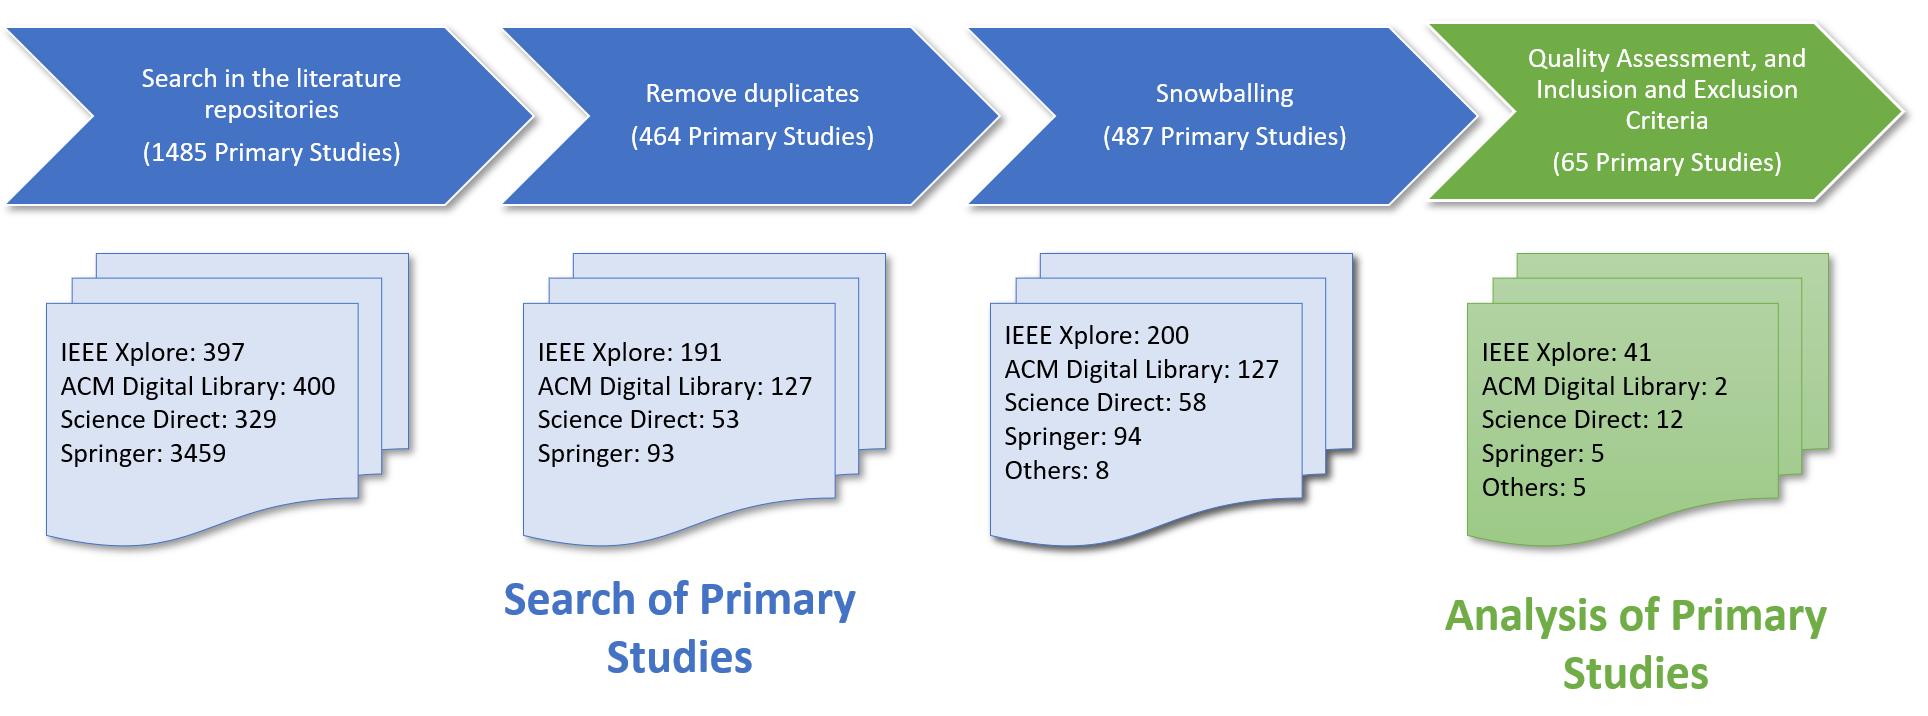
\includegraphics[width=.95\linewidth]{ResearchProcess1}
	\caption{The resulting primary studies after each action carried out in the two stages: search of primary studies and analysis of primary~studies.}
	\label{fig:1}

\end{figure}
\unskip

\subsection{Analysis of Primary~Studies} \label{sec:2.3}

We filtered the 487 primary studies based on the analysis of the titles, abstracts, and~conclusions using the inclusion and exclusion criteria, and~the assessment questions (see Figure~\ref{fig:1}). We finally selected 65 primary studies (see Table~\ref{tab:5}), which were used to answer the four RQs (see Section~\ref{sec:2.1}).
%%table 4 is cited before table 3, please modify it



\begin{table}[H]
	\centering
	\caption{The identifier, title, and reference of the 65 selected primary studies (SPS) used in this SLR.} \label{tab:5}
	\begin{tabular}{p{33pt}p{320pt}p{47pt}}
		\toprule
		\textbf{ID SPS} & \textbf{Title} & \textbf{Type of Publication}\\
		\midrule
		
		
		
		SPS \newtag{1}{que:1} & A Bionic Hand Controlled by Hand Gesture Recognition Based on Surface EMG Signals: A Preliminary Study %Please ensure consistency of capitalisation formatting for all titles.
		~\cite{Shi2018a}& Journal\\
		\midrule
		SPS \newtag{2}{que:2}& Real-Time Hand Gesture Recognition Based on Electromyographic Signals and Artificial Neural Networks %Please ensure there is a space before every reference citation throughout entire paper.
		~\cite{motoche2018real}& Conference \\
		\midrule
		SPS \newtag{3}{que:3}&sEMG-Based Continuous Hand Gesture Recognition Using GMM-HMM and Threshold Model~\cite{Yang2018}& Conference \\
		
		\midrule
		
		SPS \newtag{4}{que:4}&Hand Gestures Recognition Using Machine Learning for Control of Multiple Quadrotors~\cite{Redrovan2018}& Symposium\\
		\midrule
		SPS \newtag{5}{que:5}& Real-Time Myocontrol of a Human--Computer Interface by Paretic Muscles After Stroke~\cite{Yang2018a} & Journal\\
		\bottomrule
\end{tabular}
\end{table}

\begin{table}[H]\ContinuedFloat
\centering
\caption{\textit{Cont}.} 
\begin{tabular}{p{33pt}p{310pt}p{57pt}}
\toprule
%\begin{tabular}{p{33pt}p{320pt}p{47pt}}
%		\caption{\textit{Cont}.} \label{tab:5}\\


\textbf{ID SPS} & \textbf{Title} & \textbf{Type of Publication}\\		


		\midrule
		SPS \newtag{6}{que:6}& Decoding of Individual Finger Movements From Surface EMG Signals Using Vector Autoregressive Hierarchical Hidden Markov Models (VARHHMM) \cite{Malesevic2015}& Conference \\
		\midrule
		SPS \newtag{7}{que:7}& User-Independent Real-Time Hand Gesture Recognition Based on Surface Electromyography~\cite{Kerber2017} & Conference\\
		\midrule
		SPS \newtag{8}{que:8}& Hand Gesture Recognition Using Machine Learning and the Myo Armband~\cite{Benalcazar2017} & Conference\\
		\midrule
		SPS \newtag{9}{que:9}& Real-Time Hand Gesture Recognition Using the Myo Armband and Muscle Activity Detection~\cite{Benalcazar2017a}& Conference\\
		\midrule
		
		
		
		
		
		SPS \newtag{10}{que:10}& A Sub-10 mW Real-Time Implementation for EMG Hand Gesture Recognition Based on a Multi-Core Biomedical SoC~\cite{Benatti2017} & Workshop\\
		\midrule
		SPS \newtag{11}{que:11}& Design and Myoelectric Control of an Anthropomorphic Prosthetic Hand~\cite{Wang2017}& Journal  \\
		\midrule
		SPS \newtag{12}{que:12}& Wearable Armband for Real Time Hand Gesture Recognition~\cite{Lian2017} & Conference\\
		\midrule
		SPS \newtag{13}{que:13}& Simple Space-Domain Features for Low-Resolution sEMG Patternn Recognition~\cite{Donovan2017}& Conference\\
		\midrule
		SPS \newtag{14}{que:14}& A Wireless Surface EMG Acquisition and Gesture Recognition System~\cite{Wu2017}& Congress\\
		\midrule
		SPS \newtag{15}{que:15}& Single Channel Surface EMG Control of Advanced Prosthetic Hands: A Simple, Low Cost and Efficient Approach~\cite{Tavakoli2017}& Journal\\
		\midrule
		SPS \newtag{16}{que:16}& The Virtual Trackpad: an Electromyography-Based, Wireless, Real-Time, Low-Power, Embedded Hand Gesture Recognition System Using an Event-Driven Artificial Neural Network~\cite{Liu2016}& Journal\\
		
		\midrule
		SPS \newtag{17}{que:17}& Muscle-Gesture Robot Hand Control Based on sEMG Signals With Wavelet Transform Features and Neural Network classifier~\cite{Luh2017}& Conference\\
		\midrule
		SPS \newtag{18}{que:18}& Evaluating Sign Language Recognition Using the Myo Armband~\cite{Abreu2016}& Symposium\\
		\midrule
		SPS \newtag{19}{que:19}& Spectral Collaborative Representation Based Classification for Hand Gestures Recognition on Electromyography Signals~\cite{Boyali2016b}& Conference\\
		\midrule
		SPS \newtag{20}{que:20}&A Convolutional Neural Network for Robotic Arm Guidance Using sEMG Based Frequency-Features~\cite{Coteallard2016}& Conference \\
		\midrule
		SPS \newtag{21}{que:21}& EMG Pattern Recognition Using Decomposition Techniques for Constructing Multiclass Classifier~\cite{Huang2016a} & Conference\\
		\midrule
		SPS \newtag{22}{que:22}& SEMG Based Human Computer Interface for Physically Challenged Patients~\cite{Shafivulla2016}& Conference \\
		\midrule
		SPS \newtag{23}{que:23}& EMG Feature Set Selection Through Linear Relationship for Grasp Recognition~\cite{Kakoty2016}& Journal\\
		\midrule
		SPS \newtag{24}{que:24}& A Portable Artificial Robotic Hand Controlled by EMG Signal Using ANN Classifier~\cite{Wang2015}& Conference\\
		\midrule
		
		SPS \newtag{25}{que:25}&Real-Time American Sign Language Recognition System by Using Surface EMG Signal~\cite{Savur2015}& Conference \\
		\midrule
		SPS \newtag{26}{que:26}&Hand Motion Recognition From Single Channel Surface EMG Using Wavelet \& Artificial Neural Network~\cite{Mane2015} & Conference\\
		\midrule
		SPS \newtag{27}{que:27}& A Versatile Embedded Platform for EMG Acquisition and Gesture Recognition~\cite{Benatti2015}& Journal \\
		\midrule
		SPS \newtag{28}{que:28}&Hybrid EMG classifier Based on HMM and SVM for Hand Gesture Recognition in Prosthetics~\cite{Rossi2015} & Conference\\
		\midrule
		SPS \newtag{29}{que:29}& Human--Computer Interaction System Design Based on Surface EMG Signals~\cite{Li2014} & Conference\\
		\midrule
		SPS \newtag{30}{que:30}&Towards EMG Control Interface for Smart Garments~\cite{Benatti2014a} & Symposium\\
		\midrule
		SPS \newtag{31}{que:31}& Identification of Low Level sEMG Signals for Individual Finger Prosthesis~\cite{Villarejo2014} & Conference\\
		\midrule
		SPS \newtag{32}{que:32}&Pattern Recognition of Eight Hand Motions Using Feature Extraction of Forearm EMG Signal~\cite{AlOmari2014} & Journal\\
		
		\bottomrule
	\end{tabular}
\end{table}

\begin{table}[H]\ContinuedFloat
	\centering
	\caption{\textit{Cont}.} 
	\begin{tabular}{p{33pt}p{320pt}p{47pt}}
		\toprule
		%\begin{tabular}{p{33pt}p{320pt}p{47pt}}
		%		\caption{\textit{Cont}.} \label{tab:5}\\
		
		
		\textbf{ID SPS} & \textbf{Title} & \textbf{Type of Publication}\\		
		
		
		\midrule
		SPS \newtag{33}{que:33}&Pattern Recognition of Number Gestures Based on a Wireless Surface EMG System~\cite{Chen2013} & Journal\\
		
		
		\midrule
		SPS \newtag{34}{que:34}& Deep Learning for Electromyographic Hand Gesture Signal Classification Using Transfer Learning~\cite{cote2019deep}& Journal\\
		\midrule
		SPS \newtag{35}{que:35}&Real-Time Hand Gesture Recognition Model Using Deep Learning Techniques and EMG Signals~\cite{chung2019real}& Conference \\
		\midrule
		SPS \newtag{36}{que:36}&Real-Time Hand Gesture Recognition Based on Artificial Feed-Forward Neural Networks and EMG~\cite{benalcazar2018real} & Conference\\
		\midrule
		SPS \newtag{37}{que:37}& Pattern Recognition-Based Real Time Myoelectric System for Robotic Hand Control~\cite{wang2019pattern}& Conference \\
		\midrule
		
		SPS \newtag{38}{que:38}&Hand Gesture Recognition and Classification Technique in Real-Time~\cite{das2019hand} & Conference\\
		\midrule
		
		SPS \newtag{39}{que:39}& Forearm Muscle Synergy Reducing Dimension of the Feature Matrix in Hand Gesture Recognition~\cite{luo2018forearm} & Conference\\
		\midrule
		
		SPS \newtag{40}{que:40}&EMG Wrist-Hand Motion Recognition System for Real-Time Embedded Platform~\cite{raurale2019emg} & Conference\\
		\midrule
		
		SPS \newtag{41}{que:41}& Robust Real-Time Embedded EMG Recognition Framework Using Temporal Convolutional Networks on a Multicore IoT Processor~\cite{zanghieri2019robust} & Journal\\
		\midrule
		
		SPS \newtag{42}{que:42}&A Multi-Gestures Recognition System Based on Less sEMG Sensors~\cite{yang2019multi} & Conference\\
		\midrule
		
		SPS \newtag{43}{que:43}&A Fully Embedded Adaptive Real-Time Hand Gesture Classifier Leveraging HD-sEMG \& Deep Learning~\cite{tam2019fully} & Journal\\
		\midrule	
		
		SPS \newtag{44}{que:44}& Real-time Pattern Recognition for Hand Gesture Based on ANN and Surface EMG~\cite{yang2019real}& Conference\\
		\midrule
		
		SPS \newtag{45}{que:45}&Adjacent Features for High-Density EMG Pattern Recognition~\cite{donovan2018adjacent}& Conference \\
		\midrule
		
		SPS \newtag{46}{que:46}&Automatic EMG-based Hand Gesture Recognition System Using Time-Domain Descriptors and Fully-Connected Neural Networks~\cite{neacsu2019automatic} & Conference\\
		\midrule
		
		SPS \newtag{47}{que:47}& Artificial Neural Network to Detect Human Hand Gestures for a Robotic Arm Control~\cite{schabron2019artificial}& Conference \\
		\midrule
		
		SPS \newtag{48}{que:48}&Electromyography-Based Hand Gesture Recognition System for Upper Limb Amputees~\cite{pancholi2019electromyography} & Journal\\
		\midrule
		
		SPS \newtag{49}{que:49}&Robust Hand Gesture Recognition With a Double Channel Surface EMG Wearable Armband and SVM classifier~\cite{tavakoli2018robust} & Journal\\
		\midrule
		
		SPS \newtag{50}{que:50}&Fuzzy Classification of Hand's Motion~\cite{peter2018fuzzy} & Conference\\
		\midrule
		
		SPS \newtag{51}{que:51}& EMG-Based Online Classification of Gestures With Recurrent Neural Networks~\cite{simao2019emg} & Journal\\
		\midrule
		
		SPS \newtag{52}{que:52}&Teleoperated Robotic Arm Movement Using Electromyography Signal With Wearable Myo Armband~\cite{hassan2019teleoperated} & Journal\\
		\midrule
		SPS \newtag{53}{que:53}&Identification of Gesture Based on Combination of Raw sEMG and sEMG Envelope Using Supervised Learning and Univariate Feature Selection~\cite{liang2019identification} & Journal\\
		\midrule		
		
		SPS \newtag{54}{que:54}& Surface EMG Hand Gesture Recognition System Based on PCA and GRNN~\cite{qi2019surface}& Journal\\
		\midrule
		
		SPS \newtag{55}{que:55}&Dexterous Hand Gestures Recognition Based on Low-Density sEMG Signals for Upper-Limb Forearm amputees~\cite{mayor2017dexterous}& Journal \\
		\midrule
		
		SPS \newtag{56}{que:56}&Real-Time Surface EMG Pattern Recognition for Hand Gestures Based on an Artificial Neural Network~\cite{zhang2019real} & Journal\\
		\midrule
		
		
		SPS \newtag{57}{que:57}&	On the Usability of Intramuscular EMG for Prosthetic Control: A Fitts' Law Approach~\cite{kamavuako2014usability}&	Journal	\\	
		\midrule
		SPS \newtag{58}{que:58}&	Validation of a Selective Ensemble-Based Classification Scheme for Myoelectric Control Using a Three-Dimensional Fitts' Law Test~\cite{scheme2012validation}&	Journal	\\
	
		
		\bottomrule
	\end{tabular}
\end{table}

\begin{table}[H]\ContinuedFloat
	\centering
	\caption{\textit{Cont}.} 
	\begin{tabular}{p{33pt}p{320pt}p{47pt}}
		\toprule
		\textbf{ID SPS} & \textbf{Title} & \textbf{Type of Publication}\\	
		
		
		
		\midrule
		SPS \newtag{59}{que:59}&	Support Vector Regression for Improved Real-Time, Simultaneous Myoelectric Control~\cite{ameri2014support}&	Journal	\\
		
	
		\midrule
		SPS \newtag{60}{que:60}&	Real-Time and Simultaneous Control of Artificial Limbs Based on Pattern Recognition Algorithms~\cite{ortiz2014real}&	Journal	\\	\midrule
		SPS \newtag{61}{que:61}&	On the Robustness of Real-Time Myoelectric Control Investigations: A Multiday Fitts' Law approach~\cite{waris2019robustness}&	Journal	\\	\midrule
		SPS \newtag{62}{que:62}&	Regression Convolutional Neural Network for Improved Simultaneous EMG Control~\cite{ameri2019regression}&	Journal	\\	\midrule
		SPS \newtag{63}{que:63}&A Comparison of the Real-Time Controllability of Pattern Recognition to Conventional Myoelectric Control for Discrete and Simultaneous Movements~\cite{young2014comparison}&	Journal	\\	\midrule
		SPS \newtag{64}{que:64}&A Real-Time Comparison Between Direct Control, Sequential Pattern Recognition Control and Simultaneous Pattern Recognition Control Using a Fitts’ Law Style Assessment Procedure~\cite{wurth2014real}&	Journal	\\	\midrule
		SPS \newtag{65}{que:65}&	Evaluation of Computer-Based Target Achievement Tests for Myoelectric Control~\cite{gusman2017evaluation}&	Journal	\\	
		
		
		\bottomrule
	\end{tabular}
\end{table}

\subsubsection{Inclusion and Exclusion~Criteria} \label{sec:2.3.1}

We established the Inclusion and Exclusion Criteria based on the RQs (see Section~\ref{sec:2.1}). These criteria were used to determine if a primary study contributes to answering the RQs. The~Table~\ref{tab:3} shows the inclusion and exclusion~criteria.

\begin{table}[H]
	\caption{Inclusion and exclusion criteria used in this systematic literature review (SLR).}
	\label{tab:3}
	\centering
%	\setlength{\tabcolsep}{3pt}
	\scalebox{.95}[.95]{\begin{tabular}{ll}
		\toprule
		\textbf{Inclusion}&Primary studies about the development of the Hand Gesture Recognition (HGR) model.\\ 
		\textbf{Criteria}&Primary studies that use electromyography (EMG) as input of the HGR model.\\
		\midrule
		&The full text of the primary study was not available.\\
		\textbf{Exclusion}&Primary studies that do not use machine learning (ML) in the HGR model.\\ 
	\multirow{3}{*}{\textbf{Criteria}}&Primary studies that do not indicate that their models are in real time.\\ 
		&Primary studies that are in another language than English.\\ 
		&Primary studies that are not peer-reviewed.\\
		
		\bottomrule
	\end{tabular}}
\end{table}
\unskip





\subsubsection{Quality~Assessment} \label{sec:2.3.2}

We defined three assessment questions to evaluate the comprehensiveness, reliability, and~applicability of the primary studies. For~each question, we established three possible answers with their scores: “Yes” = 1, “Partly” = 0.5, and~“No” = 0. Thus, a~primary study was rejected if the mean of the three answers is less than 2. The~three assessment questions are:

\begin{itemize} 
	
	\item Were the research objectives of the primary studies clear?
	\item Was the contribution of the primary study clear?
	\item Was the structure of the HGR model shown?
\end{itemize}




\subsection{Data~Extraction} \label{sec:2.4}
We extracted the data shown in Table~\ref{tab:6} from the 65 selected primary studies (SPS), shown in Table~\ref{tab:5}. This extraction was performed in order to answer the four RQs (see Section~\ref{sec:2.1}). 




	
%\end{longtable}










\begin{table}[H]
\centering
	\caption{The data extracted from the 65 SPS and their targets.}
	\label{tab:6}
	
%	\setlength{\tabcolse^{}p}{3pt}
	\begin{tabular}{ll}
		\toprule
		\textbf{Extracted Data}&\textbf{Target}\\
		\midrule
		Publication year&Study overview\\
		
		Primary study type&Study overview\\
		
		Structure of the HGR model&RQ1\\
		
		Controller delay of the HGR model&RQ2\\
		
		Hardware used&RQ2\\
		
		Number of gestures recognized&RQ3\\
		
		Types of gestures recognized&RQ3\\
		
		Metrics and results used to evaluate the HGR models&RQ4\\
		
		\bottomrule
	\end{tabular}
\end{table}
\unskip



\subsection{Threats to~Validity}

We discuss the following possible threats to the validity of this SLR and the mitigation of these threats: an incomplete selection of the SPS, inaccurate data extraction, and~biased quality~assessment.

\subsubsection{Incomplete Selection of the~SPS}

There is a possibility that relevant studies have been omitted for two reasons. The~literature repositories may not have had all relevant studies for the four RQs, and~the search strings may not have been appropriate for the four RQs. However, the~authors performed the following three actions to mitigate these two threats: (1) We developed this SLR based on the Kitchenham methodology~\cite{kitchenham2004procedures,kitchenham2009systematic}, which was shown in Section~\ref{sec:2}. (2) In this SLR, the~four literature repositories and the ten search strings were proposed by the first author, and~the second and third authors assessed the relevance of these literature repositories and search strings. The~four literature repositories were assessed in accordance with the criterion that these repositories are the most used in the ML area. The~ten search strings were assessed based on the criterion that the keywords and the structures of the search strings are relevant to the four RQs. (3) We applied the snowballing techniques~\cite{wohlin2014guidelines} to add 14 SPS to the SLR. This task was performed by the first author, and~the third author assessed the relevance of these 14~SPS.  


\subsubsection{Biased Analysis of Primary~Studies}

The analysis of the primary studies (see Section~\ref{sec:2.3}) can be biased for two reasons. The~inclusion and exclusion criteria may not be relevant to the four RQs, and~the SPS may not be comprehensive, reliable, and~applicable. To~mitigate these two threats, the~authors performed the following two actions: (1) The authors developed formal inclusion and exclusion criteria (see Section~\ref{sec:2.3.1}) and quality assessment criteria (see Section~\ref{sec:2.3.2}). These criteria were proposed by the first author, and~they were assessed by the second and third authors. (2) The first author selected 65 primary studies reading the title, abstract, and~conclusions. However, the~first author also read the whole study when the title, abstract, and~conclusions were not clear. Furthermore, these 65 SPS were assessed by the second and third~authors.

\subsubsection{Inaccurate Data~Extraction}
Generally, the~data extracted can be inaccurate for two possible problems: unsystematic data extraction, and~the data not being relevant to the RQs. To~solve these problems, we extracted the data using a systematic methodology based on the four RQs (see Section~\ref{sec:2.4}). Moreover, the~authors made sure that the extracted data answer the four~RQs.





\section{Results and~Discussion} \label{result}

The data extracted from the 65 SPS (see Table~\ref{tab:5}) are presented and analyzed in five subsections: the study overview subsection and the other four subsections, one per each RQ (see Section~\ref{sec:2.1}). Although~some SPS presented more than one HGR model, we selected the models with the best performance in the evaluation; therefore, we used 65 HGR models for this~review.

\subsection{Study~Overview}
The study overview shows a general vision of the settings used in the SPS. Among~other data, we decided to extract the publication year and the type of publication. Figure~\ref{fig:2}a shows the number of SPS per year, which has increased steadily since 2013. Moreover, in~Figure~\ref{fig:2}b, we show that most of the SPS were presented in conferences, also see Table~\ref{tab:5}.




\begin{figure}[H]
	\centering
	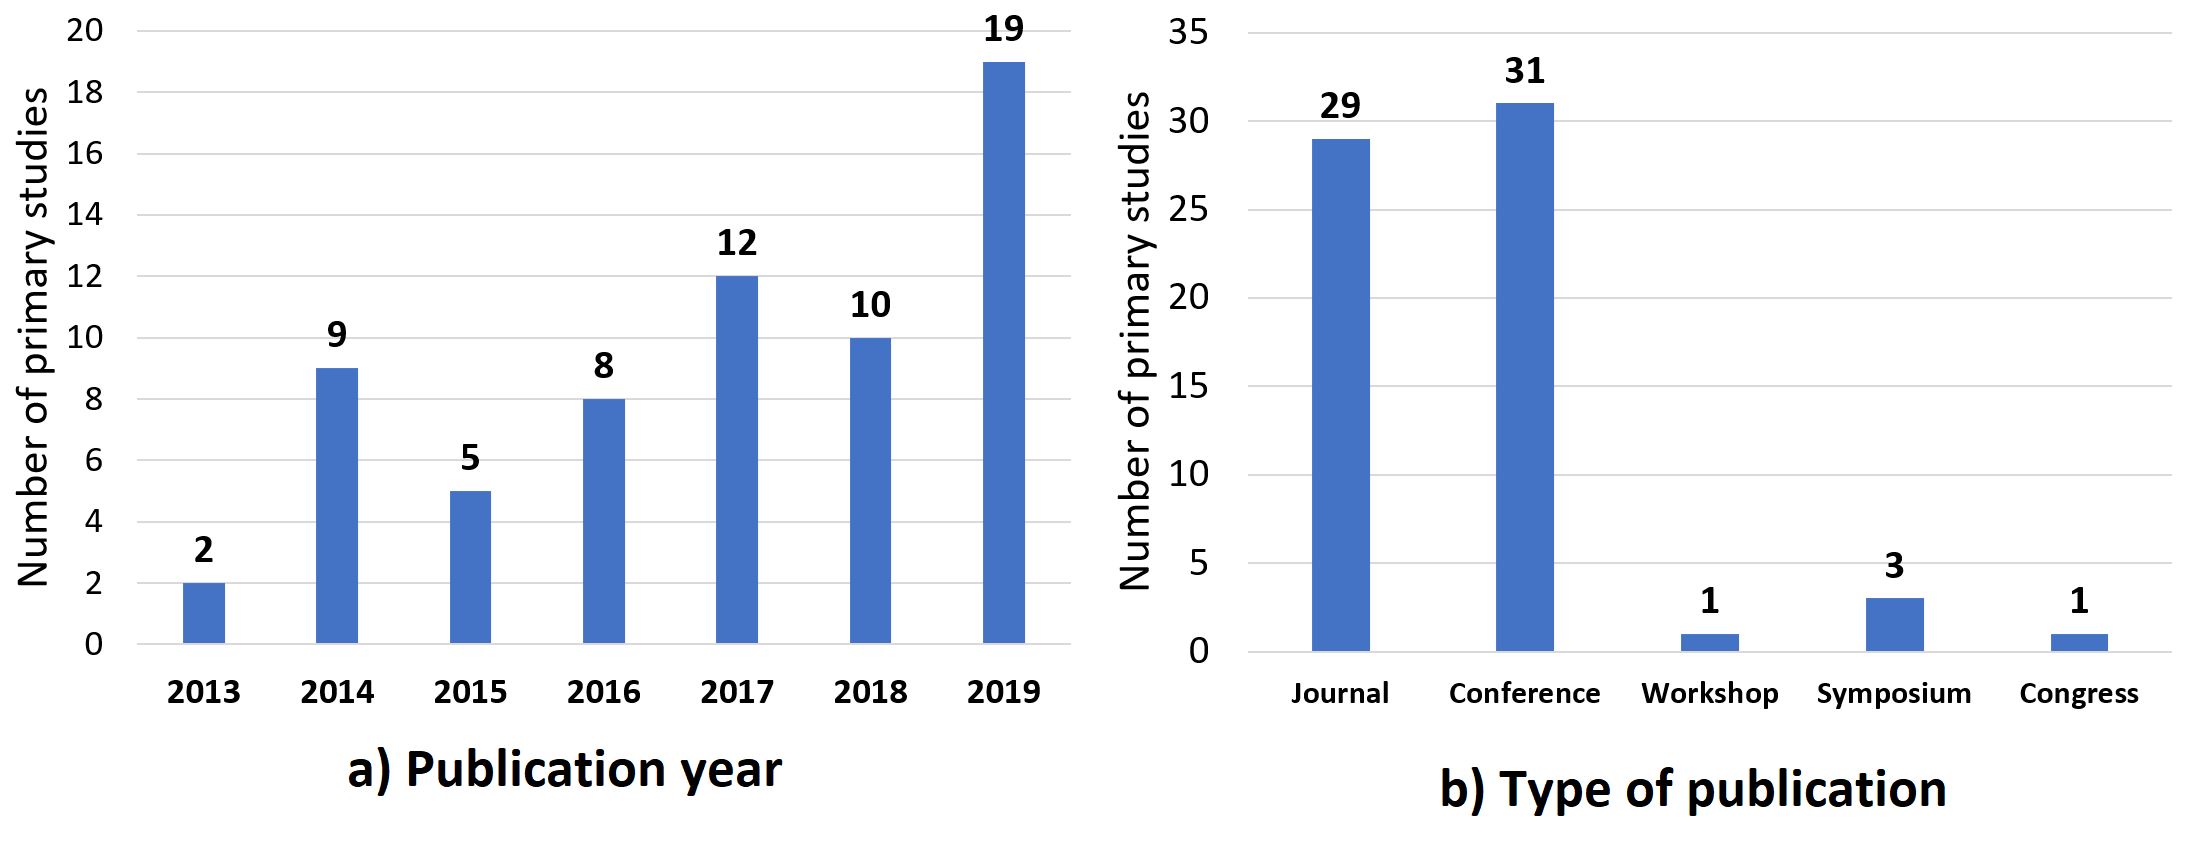
\includegraphics[width=\linewidth]{PublicationYear}
	\caption{Number of the SPS published per (\textbf{a}) year and per (\textbf{b}) type of~publication.}
	\label{fig:2}

\end{figure}
\unskip

\subsection{Results of the RQ1 (What Is the Structure of Real-Time HGR Models Using EMG and ML?)} \label{RQ1}

We found that the structures of the 65 real-time HGR models are not regular across the studies. However, they have some stages in common, such as Data Acquisition (DA), Segmentation (SEGM), Preprocessing (PREP), Feature Extraction (FE), Classification (CL), and~Postprocessing (POSTP). We present a standard structure, considering the frequent stages after they were assembled, the~result is illustrated in Figure~\ref{fig:3}. Note that there are SPS that did not use all stages of the standard structure because Segmentation, Preprocessing, Feature Extraction, and~Postprocessing are optional stages (i.e., without~them a model is still feasible). Table~\ref{tab:7} shows the stages of the standard structure used by the~SPS.


\begin{figure}[H]
	\centering
	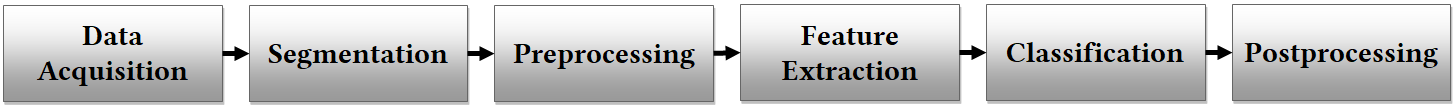
\includegraphics[width=\linewidth]{commonStructure}
	\caption{The six stages of the standard structure of the~SPS.}
	\label{fig:3}

\end{figure}



Aside from the structure of the models, we identified two types of models: the individual models and the general models. Individual models are trained relying on the gestures (data) of a person and recognize the gestures of that same person. General models are trained with the data of several people and recognize the gestures of any person. We found 44 SPS that developed individual models (SPS \ref{que:1}, SPS \ref{que:2}, SPS \ref{que:3}, SPS \ref{que:5}, SPS \ref{que:6}, SPS \ref{que:8}, SPS \ref{que:9}, SPS \ref{que:10}, SPS \ref{que:13}, SPS \ref{que:15}, SPS \ref{que:16}, SPS \ref{que:24}, SPS \ref{que:25}, SPS \ref{que:27}, SPS \ref{que:28}, SPS \ref{que:30}, SPS \ref{que:33}, SPS \ref{que:34}, SPS \ref{que:36}, SPS \ref{que:37}, SPS \ref{que:38}, SPS \ref{que:39}, SPS \ref{que:41}, SPS \ref{que:42}, SPS \ref{que:43}, SPS \ref{que:44}, SPS \ref{que:45}, SPS \ref{que:47}, SPS \ref{que:48}, SPS \ref{que:49}, SPS \ref{que:51}, SPS \ref{que:52}, SPS \ref{que:53}, SPS \ref{que:55}, SPS \ref{que:56}, SPS \ref{que:57}, SPS \ref{que:58}, SPS \ref{que:59}, SPS \ref{que:60}, SPS \ref{que:61}, SPS \ref{que:62}, SPS \ref{que:63}, SPS \ref{que:64}, and~SPS \ref{que:65}), and~11 SPS that developed general models (SPS \ref{que:7}, SPS \ref{que:11}, SPS \ref{que:17}, SPS \ref{que:22}, SPS \ref{que:23}, SPS \ref{que:26}, SPS \ref{que:31}, SPS \ref{que:32}, SPS \ref{que:35}, SPS \ref{que:40}, and~SPS \ref{que:46}). The~10 remaining studies do not indicate any type of HGR model. Out of the 11 general models, SPS \ref{que:35} is the only general model that was evaluated using EMG data from people who did not participate in the training phase. The~other 10 general models only used EMG data from people who participated in the training; therefore, it is not possible to conclude that these 10 models are able to recognize gestures of any~person.



\begin{table}[H]
\centering
	\caption{Standard structure used by the 65 HGR models.} \label{tab:7}
	
	\begin{tabular}{ccccccccc}

	\toprule
	\multirow{2}{*}{\textbf{ID SPS}\vspace{-5pt}}&\multicolumn{6}{c}{\textbf{Stages of the Standard Structure}}\\ \cmidrule{2-7}
	
	
	
	&\textbf{DA}&\textbf{SEGM}&\textbf{PREP}&\textbf{FE}&\textbf{CL} &\textbf{POSTP}\\
\midrule
	
	
	
%	
%	\endfirsthead
%	\multicolumn{7}{c}%
%	{\tablename\ \thetable\ -- \textit{Continued from previous page}} \\
%	
%	\vspace{\fill}\textbf{ID SPS}\vspace{\fill} &\multicolumn{6}{c}{\textbf{Stages of the Standard Structure}}\\ \cline{2-7}
%	
%	
%	
%	&DA&SEGM&PREP&FE&CL &POSTP\\
%
%	
%	
%	\endhead
%	 \multicolumn{7}{r}{\textit{Continued on next page}} \\
%	\endfoot
%	
%	\endlastfoot



		SPS \ref{que:1}& yes  & yes& no& yes& yes& no\\
		
		SPS \ref{que:2}& yes & yes& yes& yes& yes& yes\\
		
		SPS \ref{que:3}& yes & yes& no& yes& yes& no\\
		
		SPS \ref{que:4}& yes & yes& no& no& yes& no\\
		
		SPS \ref{que:5}& yes & yes& no& yes& yes& no\\
		
		SPS \ref{que:6}& yes & yes& no& yes& yes& no\\
		
		SPS \ref{que:7}& yes & yes& no& yes& yes& no\\
		
		SPS \ref{que:8}& yes & yes& yes& no& yes& yes\\
		
		SPS \ref{que:9}& yes & yes& yes& no& yes& yes\\
		
		SPS \ref{que:10}& yes & yes& yes& yes& yes& no\\
		
		SPS \ref{que:11}& yes & yes& yes& yes& yes& yes\\
		
		SPS \ref{que:12}& yes & no& yes& yes& yes& no\\
		
		SPS \ref{que:13}& yes & yes& no& yes& yes& no\\
		
		SPS \ref{que:14}& yes & no& yes& yes& yes& no\\
		
		SPS \ref{que:15}& yes & yes& yes& yes& yes& no\\
		
		SPS \ref{que:16}& yes & yes& yes& yes& yes& no\\
		
		SPS \ref{que:17}& yes & no& yes& yes& yes& no\\
		
		SPS \ref{que:18}& yes & no& no& yes& yes& no\\
		
		SPS \ref{que:19}& yes & yes& no& yes& yes& no\\
		
		SPS \ref{que:20}& yes & yes& no& yes& yes& no\\
		
		SPS \ref{que:21}& yes & yes& yes& yes& yes& yes\\
		
		SPS \ref{que:22}& yes & no& yes& yes& yes& no\\
		
		SPS \ref{que:23}& yes & no& yes& yes& yes& no\\
		
		SPS \ref{que:24}& yes &no&no& yes& yes& no\\
		
		SPS \ref{que:25}& yes & yes& yes& yes& yes& no\\
		
		SPS \ref{que:26}& yes & yes& no& yes& yes& no\\
		
		SPS \ref{que:27}& yes & yes& yes& no& yes& no\\
		
		SPS \ref{que:28}& yes & no& yes& no& yes& no\\
		
		SPS \ref{que:29}& yes & no& yes& yes& yes&no\\
		
		SPS \ref{que:30}& yes & yes& yes& no& yes& no\\
		
		SPS \ref{que:31}& yes & yes& yes& yes& yes& no\\
		
		SPS \ref{que:32}& yes & yes& yes& yes& yes& no\\
		
		SPS \ref{que:33}& yes & yes& yes& yes& yes& no\\
		
		SPS \ref{que:34}&	yes	&	yes	&	no	&	yes	&	yes	&	no	\\
		
		SPS \ref{que:35}&	yes	&	yes	&	yes	&	no	&	yes	&	yes	\\
		
		SPS \ref{que:36}&	yes	&	no	&	yes	&	yes	&	yes	&	no	\\
		
		SPS \ref{que:37}&	yes	&	yes	&	yes	&	yes	&	yes	&	no	\\
		
		SPS \ref{que:38}&	yes	&	no	&	yes	&	yes	&	yes	&	no	\\
		
		SPS \ref{que:39}&	yes	&	yes	&	yes	&	yes	&	yes	&	no	\\
		
		SPS \ref{que:40}&	yes	&	yes	&	no	&	yes	&	yes	&	no	\\
		
		SPS \ref{que:41}&	yes	&	yes	&	yes	&	no	&	yes	&	yes	\\
		
		SPS \ref{que:42}&	yes	&	yes	&	yes	&	yes	&	yes	&	yes	\\
		SPS \ref{que:43}&	yes	&	yes	&	yes	&	yes	&	yes	&	no	\\
		
		SPS \ref{que:44}&	yes	&	yes	&	no	&	yes	&	yes	&	no	\\
		
		SPS \ref{que:45}&	yes	&	yes	&	no	&	no	&	yes	&	no	\\
		
		SPS \ref{que:46}&	yes	&	yes	&	no	&	yes	&	yes	&	no	\\
		
		SPS \ref{que:47}&	yes	&	no	&	yes	&	no	&	yes	&	yes	\\
		
		SPS \ref{que:48}&	yes	&	yes	&	yes	&	yes	&	yes	&	yes	\\
		
		SPS \ref{que:49}&	yes	&	yes	&	no	&	yes	&	yes	&	no	\\
		
		SPS \ref{que:50}&	yes	&	yes	&	yes	&	yes	&	yes	&	no	\\
		
		
		\bottomrule
	\end{tabular}
\end{table}

	\begin{table}[H]\ContinuedFloat
	\centering
\caption{\textit{Cont}.}
\begin{tabular}{cccccccccc}
	\toprule
	\multirow{2}{*}{\textbf{ID SPS}\vspace{-5pt}
}&\multicolumn{6}{c}{\textbf{Stages of the Standard Structure}}\\ \cmidrule{2-7}
	
	
	
	&\textbf{DA}&\textbf{SEGM}&\textbf{PREP}&\textbf{FE}&\textbf{CL} &\textbf{POSTP}\\
\midrule
		
		
		SPS \ref{que:51}&	yes	&	yes	&	yes	&	yes	&	yes	&	no	\\
		
		SPS \ref{que:52}&	yes	&	no	&	no	&	yes	&	yes	&	yes	\\
		
		SPS \ref{que:53}&	yes	&	yes	&	no	&	yes	&	yes	&	no	\\
		
		SPS \ref{que:54}&	yes	&	yes	&	yes	&	yes	&	yes	&	no	\\
		
		SPS \ref{que:55}&	yes	&	no	&	no	&	yes	&	yes	&	no	\\
		
		SPS \ref{que:56}&	yes	&	yes	&	yes	&	yes	&	yes	&	no	\\
				
		
		
		SPS \ref{que:57}&	yes	&	yes	&	yes	&	yes	&	yes	&	no	\\	
		SPS \ref{que:58}&	yes	&	yes	&	yes	&	no	&	yes	&	no	\\	
		SPS \ref{que:59}&	yes	&	yes	&	yes	&	yes	&	yes	&	no	\\	
		SPS \ref{que:60}&	yes	&	yes	&	no	&	yes	&	yes	&	yes	\\	
		SPS \ref{que:61}&	yes	&	yes	&	no	&	yes	&	yes	&	no	\\	
		SPS \ref{que:62}&	yes	&	yes	&	yes	&	no	&	yes	&	no	\\	
		SPS \ref{que:63}&	yes	&	yes	&	yes	&	yes	&	yes	&	yes	\\	
		SPS \ref{que:64}&	yes	&	yes	&	yes	&	yes	&	yes	&	yes	\\	
		SPS \ref{que:65}&	yes	&	yes	&	yes	&	yes	&	yes	&	yes	\\	
		\bottomrule
	\end{tabular}\\
\begin{tabular}{@{}c@{}} 
\multicolumn{1}{p{\textwidth -.88in}}{\footnotesize \textbf{yes:} The model used this stage;\textbf{ no}: The model did not use this stage; \textbf{DA}: Data Acquisition Stage; \textbf{SEGM}: Segmentation Stage; \textbf{PREP}: Preprocessing Stage; \textbf{FE}: Feature Extraction Stage;  \textbf{CL}: Classification stage; \textbf{POSTP}: Postprocessing Stage.}
\end{tabular}


		
%		\multicolumn{7}{p{255pt}}{\scriptsize   }\\ 
	
		
		


	
\end{table}








\subsubsection{Data~Acquisition} \label{acqui}


In the Data Acquisition stage, EMGs are acquired from EMG sensors, which can be part of homemade or commercial devices. Table~\ref{tab:8} shows the number of sensors, the~sampling rates, and~the acquisition devices used in the HGR models. We found that 27 HGR models used eight sensors, 21 of them (SPS \ref{que:2}, SPS \ref{que:3}, SPS \ref{que:4}, SPS \ref{que:7}, SPS \ref{que:8}, SPS \ref{que:9}, SPS \ref{que:13}, SPS \ref{que:17}, SPS \ref{que:18}, SPS \ref{que:19}, SPS \ref{que:20}, SPS \ref{que:34}, SPS \ref{que:35}, SPS \ref{que:36}, SPS \ref{que:40}, SPS \ref{que:44}, SPS \ref{que:46}, SPS \ref{que:47}, SPS \ref{que:52}, SPS \ref{que:56}, and~SPS \ref{que:61}) used the commercial device Myo armband that has eight sensors with a corresponding sampling rate of 200 Hz, and~the other six (SPS \ref{que:5}, SPS \ref{que:25}, SPS \ref{que:27}, SPS \ref{que:59}, SPS \ref{que:62}, and~SPS \ref{que:63}) used homemade devices with a similar design to the Myo armband, their sampling rates are 1000 Hz, 960 Hz, 1000 Hz, 1000 Hz, 1200 Hz, and~1000 Hz, respectively.

 Additionally, the~EMG sampling rate of 16 HGR models (SPS \ref{que:1}, SPS \ref{que:5}, SPS \ref{que:10}, SPS \ref{que:11}, SPS \ref{que:26}, SPS \ref{que:27}, SPS \ref{que:30}, SPS \ref{que:31}, SPS \ref{que:32}, SPS \ref{que:37}, SPS \ref{que:38}, SPS \ref{que:39}, SPS \ref{que:43}, SPS \ref{que:48}, SPS \ref{que:49}, and~SPS \ref{que:55}) is 1000 Hz because these SPS indicate that the sampling rate must be at least twice the highest frequency of the EMG, according to the Nyquist sampling theory, and~approximately 95\% of the signal power in the EMG is below 400--500 Hz~\cite{Clancy2002,GuanglinLi2010,Winter1990}). 
Table~\ref{tab:8} also shows the use of commercial devices, including the Myo armband from Thalmic Labs Inc., the~MA300 from Motion Lab Systems Inc., the~Bio Radio 150 from Cleveland Medical Devices Inc., the~ME6000 from Mega Electronics Ltd., the~Analog Front End (ADS1298) from Texas Instruments, the~Telemyo 2400T G2 from Noraxon, and~the EMG-USB2 from OT Bioelettronica. Furthermore, two models (SPS \ref{que:43} and SPS \ref{que:45}) use high-density EMG~sensors.


\begin{table}[H]
\centering
\caption{The number of sensors, sampling rate, acquisition devices, segmentation techniques, and preprocessing techniques used in the 65 HGR models.} \label{tab:8}
\begin{tabular}{m{30pt}m{44pt}m{40pt}m{113pt}m{67pt}m{70pt}}
\toprule
\textbf{ID SPS}&\textbf{Number of Sensors}&\textbf{Sampling Rate (Hz)}&\textbf{Acquisition Device Used}&\textbf{Segmentation Technique Used}&\textbf{Preprocessing Techinique Used}\\
	\midrule
%	
%	\endfirsthead
%	\multicolumn{6}{c}%
%	{\tablename\ \thetable\ -- \textit{Continued from previous page}} \\
%	
%	\textbf{ID SPS}&\textbf{Number of Sensors}&\textbf{Sampling Rate (Hz)}&\textbf{Acquisition Device Used}&\textbf{Segmentation Technique Used}&\textbf{Preprocessing Techinique Used}\\
%	
%	\endhead
%	 \multicolumn{6}{r}{\textit{Continued on next page}} \\
%	\endfoot
%	
%	\endlastfoot




		SPS \ref{que:1}	&	2	&	1000	&	 MA300 &ASW&NI\\
								
		SPS \ref{que:2}	&	8	&	200	&	Myo armband&OSW&FL and~RE\\
								
		SPS \ref{que:3}	&	8	&	200	&	Myo armband& OSW and GD&NI \\
								
		SPS \ref{que:4}	&	8	&	200	&	Myo armband&ASW&NI\\
%		\bottomrule
%	\end{tabular}
%	\end{table}
%
%	\begin{table}[H]\ContinuedFloat
%	\centering
%\caption{\textit{Cont}.}
%\begin{tabular}{m{33pt}m{40pt}m{40pt}m{115pt}m{60pt}m{70pt}}
%		\toprule
%	\textbf{ID SPS}&\textbf{Number of Sensors}&\textbf{Sampling Rate (Hz)}&\textbf{Acquisition Device Used}&\textbf{Segmentation Technique Used}&\textbf{Preprocessing Techinique Used}\\
%	\midrule
		
								
		SPS \ref{que:5}	&	8	&	1000	&	Homemade device& OSW&NI\\
								
		SPS \ref{que:6}	&	16	&	1600	&	Homemade device& OSW&NI\\
								
		SPS \ref{que:7}	&	8	&	200	&	Myo armband& OSW and GD&NI\\
								
		SPS \ref{que:8}	&	8	&	200	&	Myo armband& OSW&FL~andRE\\
								
		SPS \ref{que:9}	&	8	&	200	&	Myo armband& OSW andGD&FL and~RE\\
								
		SPS \ref{que:10}	&	3	&	1000	&	Homemade device&ASW&FL and~OC\\
								
		SPS \ref{que:11}	&	2	&	1000	&	Homemade device& ASW&PreS\\
								
		SPS \ref{que:12}	&	3	&	NI	&	Homemade device& NI&FLandRE\\
								
		SPS \ref{que:13}	&	8	&	200	&	Myo armband& OSW&NI\\
								
		SPS \ref{que:14}	&	3	&	NI	&	Homemade device&NI&FL \\
								
		SPS \ref{que:15}	&	1	&	NI	&	Homemade device& ASW and GD&RE\\
								
		SPS \ref{que:16}	&	4	&	1600	&	Homemade device& ASW and GD&RE\\
								
		SPS \ref{que:17}	&	8	&	200	&	Myo armband & NI&FL\\
								
		SPS \ref{que:18}	&	8	&	200	&	Myo armband& NI&NI\\
								
		SPS \ref{que:19}	&	8	&	200	&	Myo armband&OSW&NI \\
								
		SPS \ref{que:20}	&	8	&	200	&	Myo armband&OSW&NI \\
								
		SPS \ref{que:21}	&	16	&	1600	&	Homemade device&OSW&FL\\
								
		SPS \ref{que:22}	&	1	&	125	&	Homemade device&NI&FL\\
								
		SPS \ref{que:23}	&	2	&	NI	&	Homemade device& NI&FL\\
								
		SPS \ref{que:24}	&	3	&	NI	&	Homemade device& NI&NI\\
								
		SPS \ref{que:25}	&	8	&	960	&	Bio Radio 150& ASW&FL\\
								
		SPS \ref{que:26}	&	1	&	1000	&	Homemade device& ASW&NI\\
								
		SPS \ref{que:27}	&	8	&	1000	&	Homemade device& GD&FL\\
								
		SPS \ref{que:28}	&	4	&	500	&	Homemade device& NI&FL\\
								
		SPS \ref{que:29}	&	4	&	NI	&	Homemade device& NI&FL\\
								
		SPS \ref{que:30}	&	4	&	1000	&	Homemade device& OSW and GD&FL, OC and~RE\\
								
		SPS \ref{que:31}	&	4	&	1000	&	Homemade device& OSW&OC\\
								
		SPS \ref{que:32}	&	4	&	1000	&	Homemade device&  ASW &FL\\
								
		SPS \ref{que:33}	&	4	&	500	&	Homemade device& ASW and GD&FL\\
		
	SPS \ref{que:34}	&	8	&	200	&	Myo armband	&	OSW	&	NI\\	
	SPS \ref{que:35}	&	8	&	200	&	Myo armband	&	OSW and GD	&	RE\\	
	SPS \ref{que:36}	&	8	&	200	&	Myo armband	&	OSW	&	FL and RE\\	
	SPS \ref{que:37}	&	2	&	1000	&	Homemade device	&	OSW and GD	&	FL and AMPL\\	
	SPS \ref{que:38}	&	1	&	1000	&	Homemade device&	OSW	&	FL\\	
	SPS \ref{que:39}	&	6	&	1000	&	ME6000&	NI	&	FL	\\	
	SPS \ref{que:40}	&	8	&	200	&	Myo armband	&	OSW	&	NI\\	
	SPS \ref{que:41}	&	8	&	4000	&	Analog Front End (ADS1298)&	OSW	&	NI	\\	
	SPS \ref{que:42}	&	2	&	NI	&	Telemyo 2400T G2 &	ASW	&	NI	\\	
	SPS \ref{que:43}	&	32	&	1000	&	Homemade device&	NI	&	FL, RE and TKEO	\\	
	SPS \ref{que:44}	&	8	&	200	&	Myo armband&	ASW	&	FL and RE	\\	
	SPS \ref{que:45}	&	128	&	2048	&	EMG-USB2&	OSW	&	FL	\\
	SPS \ref{que:46}	&	8	&	200	&	Myo armband	&	ASW	&	NI	\\	
	SPS \ref{que:47}	&	8	&	200	&	Myo armband &	OSW	&	FL and NORM	\\	
	SPS \ref{que:48}	&	8	&	1000	&	Analog Front End (ADS1298)&	OSW	&	FL	\\	
	SPS \ref{que:49}	&	2	&	1000	&	Homemade device&	NI	&	FL and NORM		\\	
	SPS \ref{que:50}	&	4	&	NI	&	Homemade device&	GD	&	FL and AMPL	\\		
	\bottomrule
	\end{tabular}
	\end{table}

	\begin{table}[H]\ContinuedFloat
	\centering
\caption{\textit{Cont}.}
\begin{tabular}{m{30pt}m{44pt}m{40pt}m{113pt}m{67pt}m{70pt}}
	\toprule
	\textbf{ID SPS}&\textbf{Number of Sensors}&\textbf{Sampling Rate (Hz)}&\textbf{Acquisition Device Used}&\textbf{Segmentation Technique Used}&\textbf{Preprocessing Techinique Used}\\
	\midrule
	
	SPS \ref{que:51}	&	16	&	200	&	Myo armband&	NI	&	NI	\\	
	SPS \ref{que:52}	&	8	&	200	&	Myo armband	&	OSW	&	NI	\\	
	SPS \ref{que:53}	&	2	&	2000	&	Homemade device	&	ASW and GD	&	FL and RE\\	
	SPS \ref{que:54}	&	16	&	NI	&	Homemade device	&	NI	&	NI	\\	
	SPS \ref{que:55}	&	4	&	1000	&	Homemade device &	OSW	&	NI	\\	
	SPS \ref{que:56}	&	8	&	200	&	Myo armband	&	OSW	&	FL and RE	\\	
	
	SPS \ref{que:57}&	4	&	1000	&	Homemade device	&	OSW	&	FL	\\	
	SPS \ref{que:58}&	6	&	1000	&	Homemade device	&	OSW	&	FL	\\	
	SPS \ref{que:59}&	8	&	1000	&	Homemade device	&	OSW	&	FL	\\	
	SPS \ref{que:60}&	4	&	2000	&	Homemade device	&	OSW	&	NI	\\	
	SPS \ref{que:61}&	8	&	200	&	Myo armband	&	OSW	&	NI	\\	
	SPS \ref{que:62}&	8	&	1200	&	Homemade device	&	OSW	&	FL	\\	
	SPS \ref{que:63}&	8-12	&	1000	&	Homemade device	&	OSW	&	FL	\\	
	SPS \ref{que:64}&	6	&	1000	&	Homemade device	&	OSW	&	FL	\\	
	SPS \ref{que:65}&	4	&	200	&	Homemade device	&	OSW	&	FL	\\	
	
		\bottomrule
	\end{tabular}\\
\begin{tabular}{@{}c@{}} 
\multicolumn{1}{p{\textwidth -.88in}}{\footnotesize  \textbf{NI}: Not indicated; \textbf{OSW}: Overlapping Sliding Windowing; \textbf{ASW}: Adjacent Sliding Windowing; \textbf{GD}: Gesture Detection;   \textbf{FL}: Filtering;  \textbf{RE}: Rectification; \textbf{OC}: Offset Compensation; \textbf{PreS}: Pre-smoothing; \textbf{AMPL}: Amplification;  \textbf{TKEO}: Teager-Kaiser-Energy Operator; \textbf{NORM}: Normalization.}
\end{tabular}
		
		
%		
%		\multicolumn{6}{p{420pt}}{\scriptsize  } \\ 
%		
%	
%		
%		
%		
%
%	
\end{table}






 





\subsubsection{Segmentation} \label{seg}

EMGs are partitioned into multiple segments or windows using different techniques, such as gesture detection and sliding windowing (see Table~\ref{tab:8}). Gesture detection computes the beginning and the end of a hand gesture, and~returns the EMG that only corresponds to muscle contraction. Therefore, the~segment lengths are variable as they depend on the duration of the hand gestures. The~sliding windowing techniques partition the EMG into fixed adjacent segments (i.e., adjacent sliding windowing) or fixed overlapping segments (i.e., overlapping sliding windowing) (see Figure~\ref{fig:4}). By~increasing the window length, up~to a certain point, the~controller delay increases, and~also the accuracy of the models increase as more data are collected for recognition~\cite{AsghariOskoei2007,Englehart2001}.




\subsubsection{Preprocessing} \label{pre}

HGR models use preprocessing techniques that transform the EMG into an input signal for Feature Extraction or for the ML algorithm if the structure of the HGR model does not have Feature Extraction (see Table~\ref{tab:7}). For~example, a~common preprocessing technique is the use of a Notch Filter at 50 or 60 Hz that eliminates the AC frequency of the powerlines (SPS \ref{que:10}). Other examples include Offset Compensation, Pre-smoothing, Filtering, Rectification, Amplification, and~the use of the Teager--Kaiser-Energy Operator (see Table~\ref{tab:8}). Offset Compensation is a technique that eliminates noise through the compensation of the average value of the EMG:
\begin{equation}
EMG_{raw}=(x_1,x_2,...,x_n)
\end{equation}
\begin{equation}
mean(EMG_{raw})=\bar{x}=\frac{\sum_{i=1}^{n}(x_i)}{n}
\end{equation}
\begin{equation}
EMG_{offset}=((x_1-\bar{x}),(x_2-\bar{x}),...,(x_n-\bar{x}))
\end{equation}
\begin{equation}
mean(EMG_{offset})=0,
\end{equation}
where, 
\begin{math}
x_{1},x_{2},… ,x_{n}
\end{math}
are the raw EMG values,
\begin{math}
\bar{x}
\end{math} 
is the average value of the signal, and~
\begin{math}
(x_1-\bar{x}),(x_2-\bar{x}),...,(x_n-\bar{x})
\end{math}
are the EMG values after the use of offset compensation. Pre-smoothing is a technique that computes the mean of the last 
\begin{math}
m
\end{math}
values of the EMG and then sets the mean to the current value \begin{math}
x_n
\end{math}
of the signal:
\begin{equation}
EMG_{raw}=(x_1,x_2,...,x_n)
\end{equation}
\begin{equation}
x_n=\frac{\sum_{i=1+n-m}^{n}(x_i)}{m},
\end{equation}
where, 
\begin{math}
x_1,x_2,… ,x_n
\end{math}
are the raw EMG values and 
\begin{math}
x_n
\end{math}
is the current value that is based on the mean of the 
\begin{math}
m
\end{math} previous values of the raw EMG. Filtering is a technique that removes some unwanted frequencies or an unwanted frequency band from the raw EMG. Rectification transforms the negative values into positive values (e.g., absolute value function). The~Teager--Kaiser-Energy Operator increases the signal-to-noise ratio to improve the muscle activity onset detection of a gesture~\cite{li2007teager}. The~most used preprocessing technique is filtering (see Table~\ref{tab:8}).








\begin{figure}[H]
	\centering
	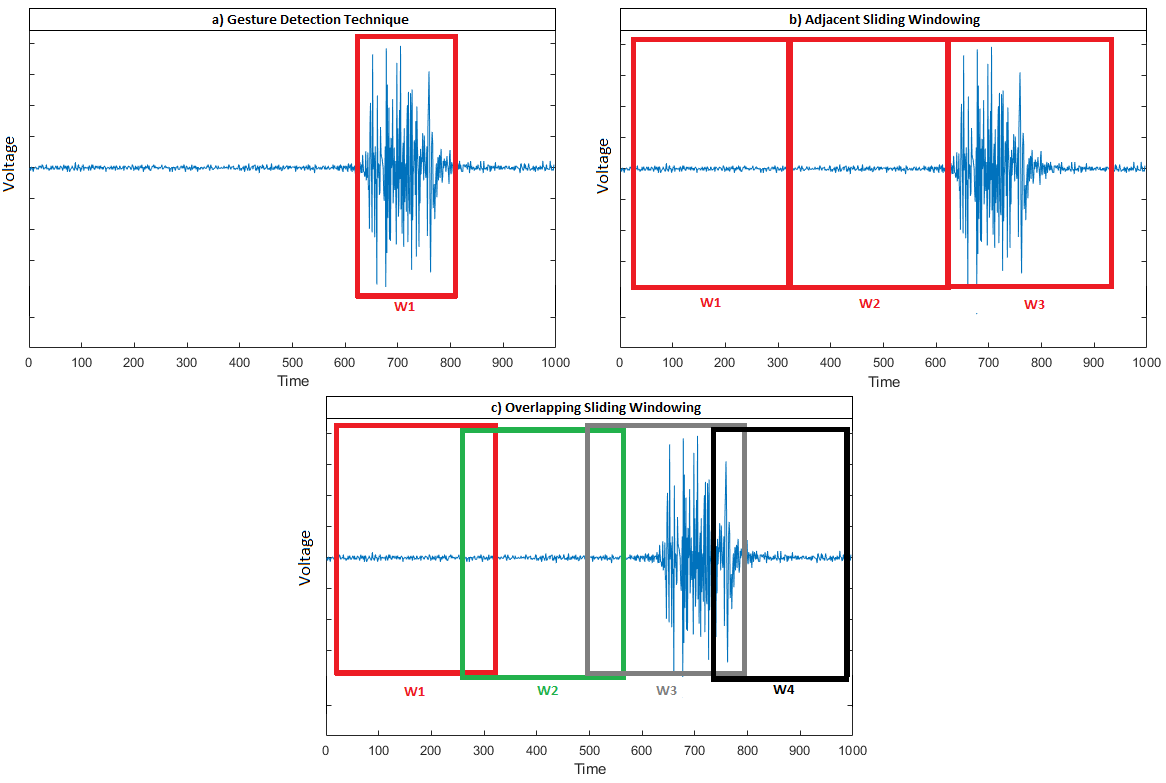
\includegraphics[width=\linewidth]{Windowing}
	\caption{Segmentation of the EMG of a gesture using the three techniques: (\textbf{a}) gesture detection, (\textbf{b})~adjacent sliding windowing, and~(\textbf{c}) overlapping sliding~windowing.}
	\label{fig:4}

\end{figure}




















\subsubsection{Feature~Extraction} \label{feat}

Feature extraction techniques map the EMG into a feature set. These techniques extract features in different domains, such as time, frequency, time-frequency, space, and~fractal. Table~\ref{tab:10a} shows the domains of the feature extraction techniques used by the models. Most of the real-time HGR models use time-domain features because the controller delay for their computation is less than the controller delay for the computation of features in other domains (see Table~\ref{tab:10}). The~mean absolute value is the most used feature in the 65 studies~analyzed.
	
	

\begin{table}[H]
	\caption{Features according to the domain.}
	\label{tab:10a}
	\centering
	\setlength{\tabcolsep}{3pt}
	\begin{tabular}{m{105pt}m{320pt}}
	
		\toprule
		
		\textbf{Time-Domain Features}& Mean absolute value (MAV),	root mean square (RMS), waveform length (WL), zero crossings (ZC), fourth-order autoregressive coefficients (AR-Coeff), 	standard deviation (SD), variance (VAR), slope sign changes (SSC), mean, median, integrated EMG (iEMG), sample entropy (SampEn), mean absolute value ratio (MAVR), modified mean absolute value (MMAV), simple square integral (SSI), Log detector (LOG), average amplitude change (AAC), maximum fractal length (MFL), minimum (MIN), maximum (MAX), Hjorth parameters (HJP), peak value (PK), energy ratio (ER), histogram (HISTG), willison amplitude (WAMP), kurtosis (KURT), skewness (SKEW), non-negative matrix factorization (NMF), natural logarithm of the variance (ln-VAR), root sum square (RSS), logarithm of the root mean square (log-RMS), logarithm  of the integrated EMG (log-iEMG),  logarithm of the variance (log-VAR), logarithmic band power (LBP), first derivation (DIFF),  detrended fluctuation analysis (DFA), modified mean absolute values (MAV1-MAV2), V-order, difference absolute standard deviation value (DASDV), max-min, autoregressive model intercept (Inpt), cardinality (CARD)   \\
		\midrule
		
		\textbf{Frequency-Domain Features}&
		
		Amplitude spectrum (AmpSpec), mean frequency (MNF), median frequency (MDF), modified median frequency (MMDF), modified mean frequency (MMNF), mean power (MNP), cepstral coefficients (Cep-Coeff), circulant matrix structure for eigenvalue decomposition (CMSED), fast Fourier transform (FFT), median amplitude spectrum (MAS), peak frequency (PKF), total power (TTP), power spectrum ratio (PSR)  \\
		\midrule
		
		
		\textbf{Time-Frequency-Domain Features}& Discrete wavelet transform (DWT), continuous wavelet transform (CWT), mean of the absolute wavelet coefficients (MOAC), average power of the wavelet coefficients (APOC), standard deviation of the wavelet coefficients (STDOC), MOAC-ratio \\
		\midrule
		\vspace{\fill}\textbf{Space-Domain Features}& Scaled mean absolute value (SMAV), mean absolute difference of the normalized values (MADN)\\
		\midrule
		\textbf{Fractal-Domain Features}&
		De-trended fluctuation analysis (DFA), Higuchi fractal dimension (HFD)\\
		\bottomrule
		
	\end{tabular}
	
\end{table}
\unskip
\begin{table}[H]
\centering
	\caption{ Features used in the 65 HGR models.} \label{tab:10}
\begin{tabular}{m{33pt}m{370pt}}
	\toprule
	\textbf{ID SPS}&\textbf{Features used}\\
	\midrule
%	
%	\endfirsthead
%	\multicolumn{2}{c}%
%	{\tablename\ \thetable\ -- \textit{Continued from previous page}} \\
%	
%	\textbf{ID SPS}&\textbf{Features used}\\
%	
%	
%	\endhead
%	 \multicolumn{2}{r}{\textit{Continued on next page}} \\
%	\endfoot
%	
%	\endlastfoot
%	
	
	SPS \ref{que:1}	&	MAV	\\	
	SPS \ref{que:2}	&	MAV, RMS, WL, SSC, and~HJP	\\	
	SPS \ref{que:3}	&	RMS	\\	
	SPS \ref{que:4}	&	NI	\\	
	SPS \ref{que:5}	&	MAV, WL, ZC, and~SSC	\\	
	SPS \ref{que:6}	&	MAV	\\	
	SPS \ref{que:7}	&	MAV, RMS, ZC, VAR, ER, HISTG, WAMP, AmpSpec, MMDF, and~MMNF	\\	
	SPS \ref{que:8}	&	NI	\\	
	SPS \ref{que:9}	&	NI	\\	
	SPS \ref{que:10}	&	RMS	\\	
	SPS \ref{que:11}	&	MAV, AR-Coeff, VAR, and~SampEn	\\	
	SPS \ref{que:12}	&	WL, VAR, iEMG, and~PK	\\	
	SPS \ref{que:13}	&	SMAV, and~MADN	\\	
	SPS \ref{que:14}	&	AR-Coeff, and~Mean	\\	
	SPS \ref{que:15}	&	Mean	\\	
	SPS \ref{que:16}	&	MAV	\\	
	SPS \ref{que:17}	&	MAV, SD, and~DWT	\\	
	SPS \ref{que:18}	&	MAV	\\	
	SPS \ref{que:19}	&	CMSED	\\	
	SPS \ref{que:20}	&	FFT	\\	
	SPS \ref{que:21}	&	MAV, WL, ZC, and~SSC	\\	
	SPS \ref{que:22}	&	RMS, SD, and~SampEn	\\	
	SPS \ref{que:23}	&	DWT	\\	
	
	\bottomrule
		
	\end{tabular}
	
\end{table}

\begin{table}[H]\ContinuedFloat
\centering
\caption{\textit{Cont}.}

\begin{tabular}{m{33pt}m{370pt}}
	\toprule
	\textbf{ID SPS}&\textbf{Features used}\\
\midrule
	SPS \ref{que:24}	&	iEMG	\\	
	SPS \ref{que:25}	&	MAV, RMS, SD, MMAV, SSI, LOG, AAC, MFL, MIN, and~MAX	\\	
	SPS \ref{que:26}	&	DWT	\\	
	SPS \ref{que:27}	&	NI	\\	
	SPS \ref{que:28}	&	NI	\\	
	SPS \ref{que:29}	&	AR-Coeff	\\	
	SPS \ref{que:30}	&	NI	\\	
	SPS \ref{que:31}	&	MAV, RMS, MNP, and~DFA	\\	
	SPS \ref{que:32}	&	DWT	\\	
	SPS \ref{que:33}	&	MAV, WL, ZC, and~MAVR	\\	
	SPS \ref{que:34}	&	CWT	\\	
	SPS \ref{que:35}	&	NI	\\	
	SPS \ref{que:36}	&	NI	\\	
	SPS \ref{que:37}	&	RMS, WL, WAMP, SampEn, and~Cep-Coeff	\\	
	SPS \ref{que:38}	&	Mean, VAR, KURT, and~SKEW	\\	
	SPS \ref{que:39}	&	NMF	\\	
	SPS \ref{que:40}	&	iEMG, ln-VAR, and~RSS	\\	
	SPS \ref{que:41}	&	NI	\\	
	SPS \ref{que:42}	&	log-RMS, log-iEMG, log-VAR	\\	
	SPS \ref{que:43}	&	NI	\\	
	SPS \ref{que:44}	&	MAV, RMS, SSC, WL, and~HJP	\\	
	SPS \ref{que:45}	&	SMAV, and~MADN	\\	
	SPS \ref{que:46}	&	MAV, ZC, SSC, SKEW, RMS,  HJP, and~iEMG	\\	
	SPS \ref{que:47}	&	RMS, and~Median	\\	
	SPS \ref{que:48}	&	RMS, WL, ZC, and~SSC	\\	
	SPS \ref{que:49}	&	Mean	\\	
	SPS \ref{que:50}	&	RMS, LBP, and~DIFF	\\	
	SPS \ref{que:51}	&	SD	\\	
	SPS \ref{que:52}	&	MAV, WL, RMS, AR-Coeff, ZC, and~SSC	\\	
	SPS \ref{que:53}	&	MAV, MAV1-MAV2, VAR, RMS, SSI, V-order, iEMG, DASDV, AAC, ZC, LOG, SSC, WL, WAMP, MFL, MAX, MIN, max-min, SKEW, KURT, TTP, MNF, MDF, MNP, PKF, MOAC, APOC, STDOC, MOAC-ratio, Inpt, AR-Coeff	\\	
	SPS \ref{que:54}	&	RMS, WL, MAS and SampEn	\\	
	SPS \ref{que:55}	&	MAV, MAV1, MAV2, VAR, RMS, WL, ZC, SSC, AR-Coeff, MNF, MDF, PKF, MNP, TTP, PSR, DFA, and~HFD	\\	
	SPS \ref{que:56}	&	MAV, SSC, WL, RMS, and~HJP	\\	
	
	
	SPS \ref{que:57}	&	MAV, WL, ZC, and~SSC	\\	
	SPS \ref{que:58}	&	NI	\\	
	SPS \ref{que:59}	&	MAV, WL, ZC, and~SSC	\\	
	SPS \ref{que:60}	&	MAV, WL, ZC, and~SSC	\\	
%	\bottomrule
%		
%	\end{tabular}
%	
%\end{table}
%
%\begin{table}[H]\ContinuedFloat
%\centering
%\caption{\textit{Cont}.}
%
%\begin{tabular}{m{33pt}m{370pt}}
%	\toprule
%	\textbf{ID SPS}&\textbf{Features used}\\
%\midrule
	SPS \ref{que:61}	&	MAV, WL, ZC, SSC, WAMP, and~CARD	\\	
	SPS \ref{que:62}	&	NI	\\	
	SPS \ref{que:63}	&	MAV, WL, ZC, and~SSC	\\	
	SPS \ref{que:64}	&	MAV, WL, ZC, and~SSC	\\	
	SPS \ref{que:65}	&	MAV, WL, ZC, and~SSC	\\	
	
	\bottomrule
		
	\end{tabular}
	
\end{table}
	
	
	
	
	
	
%\end{longtable}

\subsubsection{Classification} \label{class}
In this stage, classifiers generate class labels (i.e., the~gestures recognized) from a feature set of the EMG. The~classifiers used are support vector machines (SPS \ref{que:7}, SPS \ref{que:10}, SPS \ref{que:14}, SPS \ref{que:15}, SPS \ref{que:18}, SPS \ref{que:23}, SPS \ref{que:25}, SPS \ref{que:27}, SPS \ref{que:28}, SPS \ref{que:30}, SPS \ref{que:38}, SPS \ref{que:39}, SPS \ref{que:49}, SPS \ref{que:52}, SPS \ref{que:53}, SPS \ref{que:55}, and~SPS \ref{que:59}), feedforward neural networks (SPS \ref{que:2}, SPS \ref{que:16}, SPS \ref{que:17}, SPS \ref{que:22}, SPS \ref{que:24}, SPS \ref{que:26}, SPS \ref{que:29}, SPS \ref{que:32}, SPS \ref{que:35}, SPS \ref{que:36}, SPS \ref{que:44}, SPS \ref{que:42}, SPS \ref{que:46}, SPS \ref{que:47}, SPS \ref{que:56}, SPS \ref{que:60}, and~SPS \ref{que:61}), linear discriminant analysis (SPS \ref{que:5}, SPS \ref{que:11}, SPS \ref{que:13}, SPS \ref{que:31}, SPS \ref{que:37}, SPS \ref{que:45}, SPS \ref{que:48}, SPS \ref{que:57}, SPS \ref{que:63}, SPS \ref{que:64}, and~SPS \ref{que:65}), convolutional neural networks (CNN) (SPS \ref{que:4},  SPS \ref{que:20}, SPS \ref{que:43}, and~SPS \ref{que:62}), CNN with transfer learning (SPS \ref{que:34}), radial basis function networks (SPS \ref{que:40}), temporal convolutional networks (SPS \ref{que:41}), k-nearest neighbors and dynamic time warping (SPS \ref{que:8}, and~SPS \ref{que:9}), collaborative-representation-based classification (SPS \ref{que:19}), k-nearest neighbors (SPS \ref{que:1}), k-nearest neighbors and decision trees (SPS \ref{que:12}), binary tree-support vector machine (SPS \ref{que:21}), vector auto-regressive hierarchical hidden Markov models (SPS \ref{que:6}), Gaussian mixture models and hidden Markov models (SPS \ref{que:3}), quadratic discriminant analysis (SPS \ref{que:33}), fuzzy logic (SPS \ref{que:50}), recurrent neural networks (SPS \ref{que:51}), generalized regression neural networks (SPS \ref{que:54}), and~one vs one classifier (\ref{que:58}). The~most commonly used ML algorithms are support vector machines, feedforward neural networks, and~linear discriminant~analysis.  


\subsubsection{Postprocessing} \label{post}
To improve the accuracy of the HGR models, the~postprocessing techniques adapt the output of the ML algorithm to the final application. Only 15 out of 65 SPS used postprocessing techniques, such as majority voting (SPS \ref{que:2}, SPS \ref{que:11}, SPS \ref{que:21}, SPS \ref{que:37} and SPS \ref{que:43}), elimination of consecutive repetitions (SPS \ref{que:8}, SPS \ref{que:9}, SPS \ref{que:36}, and~SPS \ref{que:51}), threshold (SPS \ref{que:35}, and~SPS \ref{que:44}), and~velocity ramps (SPS \ref{que:60}, SPS \ref{que:63}, SPS \ref{que:64}, and~SPS \ref{que:65}). 

Many works perform an analysis of some of the stages shown in Section~\ref{RQ1} to determine the best structure to improve the accuracy of the HGR models, for~example, data acquisition~\cite{toledo2019study,li2010quantifying,hargrove2007real,Englehart2003}, optimal window length~\cite{Smith2011}, filtering~\cite{chowdhury2013surface,disselhorst1997improvement}, feature extraction~\cite{phinyomark2018feature}, and~classification~\cite{toledo2019support,nazmi2016review} stages. However, the~results are inconclusive because the structure of the HGR models depend on the environment in which the models are developed (i.e., the~data sets used, the~people who participated in the evaluation, the~application of the models, etc.)  

\subsection{Results of the RQ2 (What Is the Controller Delay and Hardware Used by Real-Time HGR Models Using EMG and ML?)}
\unskip

\subsubsection{Controller Delay of the HGR~Models } \label{time}

The controller delay is the sum of two values, which are the data collection time (DCT) (i.e., window length) and the data analysis time (DAT) \cite{Englehart2003,Farrel2007}. In~real-time processing, the~DCT and DAT should be as short as possible, but~the DCT also should allow the HGR model to collect enough EMG data to recognize a hand gesture. For~instance, in~prosthesis control, the~optimal DCT using four EMG sensors with a sampling rate of 1 kHz should be between 150--250 ms~\cite{Smith2011}.

An HGR model using EMG is considered to work in real-time when the response time (i.e., controller delay) is less than the optimal controller delay. There are several optimal controller delays reported in the scientific literature, namely 300 ms~\cite{Englehart2003}, 500 ms~\cite{Graupe1983}, and~100 ms for fast prosthetic prehensors and 125 ms for slower prosthetic prehensors %Please confirm word use is appropriate.
~\cite{Farrel2007}. 

In accordance with the Inclusion and Exclusion Criteria (see Section~\ref{sec:2.3.1}), all 65 HGR models indicate that they are real-time models. However, there are some SPS that did not report the controller delay (i.e., DCT and DAT) of their HGR models. Table~\ref{tab:11} shows the DCT and DAT of the~SPS.

\subsubsection{Hardware~Used}

The controller delay of the HGR models not only depends on their structure but also on the hardware used to process the models. For~example, an~HGR model may not work in real-time if the user perceives delays in the HGR response because the device has limited processing capabilities. The~same HGR model may also be considered to work in real-time in another device with better processing capabilities. For~this reason, when a model is described, it is fundamental to indicate the hardware characteristics of the devices used for running an HGR model. Table~\ref{tab:11} shows the two types of hardware used, which are personal computers and embedded systems. Ten HGR models were processed in personal computers, such as laptops, desktops, etc., five HGR models were processed in embedded systems, and~the remaining models did not indicate the hardware~used. 

		
\begin{table}[H]
\centering
\caption{Time of data collection and data analysis, and hardware used in the 65 HGR models.} \label{tab:11}
	\begin{tabular}{p{33pt}p{40pt}p{40pt}p{100pt}}
	\toprule
		\textbf{ID SPS}&\textbf{DCT(ms)}&\textbf{DAT(ms)}&\textbf{Hardware Used}\\
	\midrule
%	\endfirsthead
%	\multicolumn{4}{c}%
%	{\tablename\ \thetable\ -- \textit{Continued from previous page}} \\
%	
%	\textbf{ID SPS}&\textbf{DCT(ms)}&\textbf{DAT(ms)}&\textbf{Hardware Used}\\
%	
%	\endhead
%	 \multicolumn{4}{r}{\textit{Continued on next page}} \\
%	\endfoot
%	
%	\endlastfoot
%			
		
		SPS \ref{que:1} 	&	250	&	NI	&	NI	\\
		
		SPS \ref{que:2}	&	1000	&	29.38	&	Personal~computer	\\
		
		SPS \ref{que:3}	&	100	&	37.9	&	Personal~computer	\\
		
		SPS \ref{que:4}	&	250	&	NI	&	NI	\\
		
		SPS \ref{que:5}	&	250	&	NI	&	NI	\\
		
		SPS \ref{que:6}	&	250	&	NI	&	NI	\\
		
		SPS \ref{que:7}	&	300	&	500	&	NI	\\
		
		SPS \ref{que:8}	&	1000	&	250	&	Personal~Computer	\\
		
		SPS \ref{que:9}	&	1000	&	193.1	&	Personal~Computer	\\
		
		SPS \ref{que:10}	&	72	&	41	&	Embedded~System	\\
		
		SPS \ref{que:11}	&	250	&	70	&	NI	\\
		
		SPS \ref{que:12}	&	NI	&	NI	&	NI	\\
		
		SPS \ref{que:13}	&	200	&	NI	&	NI	\\
		
		SPS \ref{que:14}	&	NI	&	NI	&	NI	\\
		
		SPS \ref{que:15}	&	NI	&	10	&	NI	\\
		
		SPS \ref{que:16}	&	250	&	0.2	&	Embedded~System	\\
		
		SPS \ref{que:17}	&	NI	&	NI	&	Personal~Computer	\\
		
		SPS \ref{que:18}	&	NI	&	NI	&	NI	\\
		
		SPS \ref{que:19}	&	500	&	NI	&	NI	\\
		
		SPS \ref{que:20}	&	285	&	15	&	Personal~Computer	\\
		
		SPS \ref{que:21}	&	250	&	7.57	&	Personal~Computer	\\
		
		SPS \ref{que:22}	&	NI	&	NI	&	NI	\\
		
		SPS \ref{que:23}	&	250	&	NI	&	NI	\\
		
		SPS \ref{que:24}	&	NI	&	NI	&	Embedded~System	\\
		
		SPS \ref{que:25}	&	2000	&	NI	&	NI	\\
		
		SPS \ref{que:26}	&	NI	&	NI	&	NI	\\
		
		SPS \ref{que:27}	&	NI	&	NI	&	Embedded~System	\\
		
		SPS \ref{que:28}	&	NI	&	NI	&	Embedded~System	\\
		
		SPS \ref{que:29}	&	NI	&	NI	&	NI	\\
		
		SPS \ref{que:30}	&	NI	&	2.5	&	Personal~Computer	\\
		
		SPS \ref{que:31}	&	250	&	NI	&	Personal~Computer	\\
		
		SPS \ref{que:32}	&	256	&	NI	&	NI	\\
		
		SPS \ref{que:33}	&	64	&	NI	&	Personal~computer	\\
				
		
		SPS \ref{que:34}	&	260	&	NI	&	NI	\\	
		SPS \ref{que:35}	&	2000	&	3	&	Personal computer	\\	
		SPS \ref{que:36}	&	2500	&	11	&	Personal computer	\\	
		SPS \ref{que:37}	&	200	&	NI	&	Personal computer	\\	
		SPS \ref{que:38}	&	100	&	NI	&	Personal computer	\\	
		SPS \ref{que:39}	&	256	&	152.71	&	NI	\\	
		SPS \ref{que:40}	&	250	&	4.5	&	Embedded System	\\	
		SPS \ref{que:41}	&	150	&	12.8	&	Embedded System	\\	
		SPS \ref{que:42}	&	200	&	46.4	&	Personal computer	\\	
		SPS \ref{que:43}	&	200	&	5	&	Embedded System	\\	
		SPS \ref{que:44}	&	NI	&	233.4	&	NI	\\	
		SPS \ref{que:45}	&	200	&	NI	&	NI	\\	
		SPS \ref{que:46}	&	250	&	NI	&	NI	\\	
		SPS \ref{que:47}	&	NI	&	NI	&	NI	\\	
		SPS \ref{que:48}	&	200	&	NI	&	Embedded System	\\	
		SPS \ref{que:49}	&	800	&	NI	&	NI	\\	
		SPS \ref{que:50}	&	400	&	NI	&	Embedded System	\\	
		SPS \ref{que:51}	&	500	&	NI	&	Personal computer	\\	
		SPS \ref{que:52}	&	240	&	NI	&	Personal computer	\\	
		SPS \ref{que:53}	&	32	&	NI	&	Personal computer	\\	
		SPS \ref{que:54}	&	NI	&	190	&	NI	\\	
		\bottomrule
		\end{tabular}
\end{table}

\begin{table}[H]\ContinuedFloat
\centering
\caption{\textit{Cont}.}
\begin{tabular}{p{33pt}p{40pt}p{40pt}p{100pt}}
	\toprule
		\textbf{ID SPS}&\textbf{DCT(ms)}&\textbf{DAT(ms)}&\textbf{Hardware Used}\\
	\midrule

		
		SPS \ref{que:55}	&	300	&	NI	&	NI	\\	
		SPS \ref{que:56}	&	400	&	227.76	&	NI	\\	
		
		SPS \ref{que:57}	&	160	&	<16	&	NI	\\	
		SPS \ref{que:58}	&	160	&	<16	&	NI	\\	
		SPS \ref{que:59}	&	200	&	2	&	NI	\\	
		SPS \ref{que:60}	&	200	&	50	&	Personal computer	\\	
		SPS \ref{que:61}	&	200	&	<50	&	NI	\\	
		SPS \ref{que:62}	&	167	&	6	&	Personal computer	\\	
		SPS \ref{que:63}	&	250	&	<50	&	NI	\\	
		SPS \ref{que:64}	&	250	&	<50	&	NI	\\	
		SPS \ref{que:65}	&	200	&	<50	&	Personal computer	\\	
		
		
			\bottomrule
		\end{tabular}\\
\begin{tabular}{ccc}
\multicolumn{1}{c}{\footnotesize \textbf{NI}: Not indicated.}
\end{tabular}


%\begin{tabular}
%		
%		\multicolumn{4}{p{200pt}}{\scriptsize  } \end{tabular}
	\end{table}

	
%\end{longtable}

\subsection{Results of the RQ3 (What Is the Number and Type of Gestures Recognized by Real-Time HGR Models Using EMG and ML?)}
\unskip

\subsubsection{Number of Gestures~Recognized}

The number of gestures recognized is the number of classes of an HGR model. There are HGR models that have the same number of gestures, and~each model has different gestures. For~example, there are two HGR models that recognize four gestures, but~the classes of the first model are thumb up, okay, wrist valgus, and~wrist varus (SPS \ref{que:14}), and~the classes of the second model are hand extension, hand grasp, wrist extension, and~thumb flexion (SPS \ref{que:22}). Hence to compare these models, it is important to consider the difference in the gestures as~well.

\subsubsection{Type of Gestures~Recognized } \label{gesture}

The hand gestures, according to the type of movement, are classified as static and dynamic. A~static gesture is made when the skeletal muscles are in constant contraction (i.e., there is no movement during the gesture), and~in a dynamic gesture, the~skeletal muscles are in contraction, but~it is not constant, which indicates that there is movement during the~gesture.








The EMG data generated by a gesture has two states: transient and steady. The~EMG data in the transient state are generated during the transition from one gesture to another, and~the EMG data in the steady state are generated when a gesture is maintained~\cite{hudgins1993new}. Moreover, the~offline classification of hand gestures using EMG data in the steady state is more accurate than in the transient state as the variance of the EMG data in the transient state varies more (i.e., non-stationary process) than in the steady state over time~\cite{Englehart2001}. However, in~the training phase, the~inclusion of EMG data in the transient state improves subject performance in a real-time virtual clothespin task~\cite{hargrove2007real,gusman2017evaluation}. 

Figure~\ref{fig:5} presents the EMG data of a person who made a long-term gesture (i.e., gestures that lasted a long time) after a relaxed position or rest gesture. In~this figure, the~EMG data in the transient state are generated during the transition from the rest gesture to the peace sign, and~the EMG data in the steady state are generated when the peace sign is maintained. The~short-term gestures (i.e., gestures that lasted only a short time) generate more EMG data in the transient state than in the steady state as most of the time is spent in transitions from one gesture to another (see Figure~\ref{fig:55}).  



The durations of the gestures used by the models are shown in Table~\ref{tab:12}. This table shows seven aspects about the gestures recognized by the HGR models reviewed in this SLR, such as the number of classes, the~number of gestures per person in the training set (NGpPT), the~number of people who participated in the training (NPT), the~number of gestures per person in the evaluation set (NGpPE), the~type of gestures recognized, the~state of the EMG data used, and~the duration of the gestures (DG). NGpPT, NPT, and~DG show the EMG data used to train the individual (\begin{math}
NGpPT\times DG 
\end{math}), and~general (\begin{math}
NGpPT\times NPT\times DG 
\end{math}) models. We found that 63 out of 65 HGR models recognized static gestures, and~only one HGR model recognized both dynamic and static gestures (SPS \ref{que:25}); moreover, no HGR model recognized only dynamic gestures. Additionally, six SPS used EMG data in the steady state, two SPS used EMG data in the transient state, three SPS used EMG data in the steady and transient states, and~the remaining HGR models did not indicate the state of the EMG data. There were 31 out of the 65 HGR models that considered the rest gesture (i.e., the~hand does not make any movement) as a~class.


\begin{figure}[H]
	\centering
	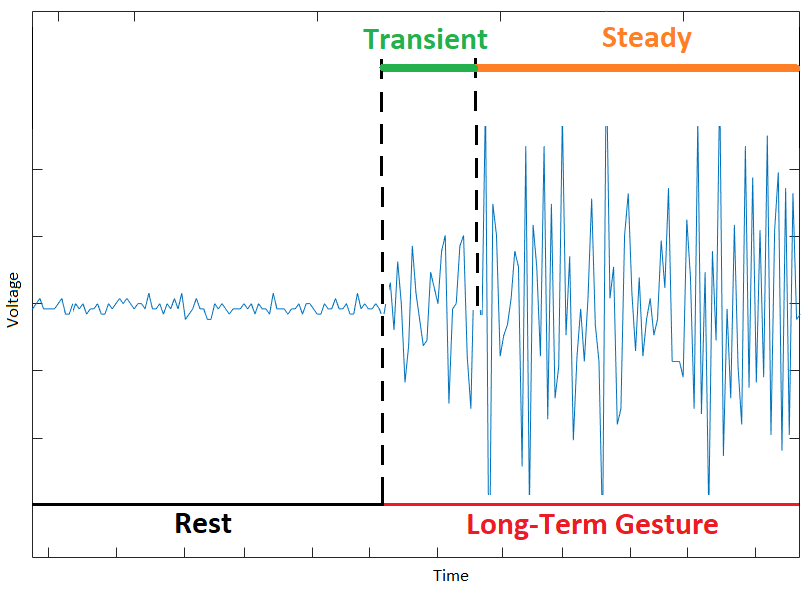
\includegraphics[scale=0.8]{transientSteadypre}
	\caption{The EMG data of a long-term peace gesture (most of the EMG data are in the steady state).}
	\label{fig:5}
	
\end{figure}
\unskip


\begin{figure}[H]
	\centering
	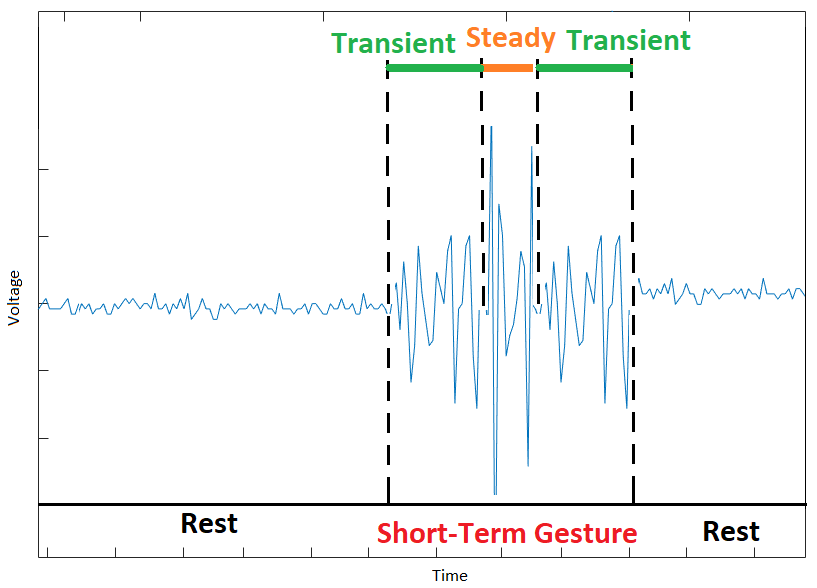
\includegraphics[scale=0.8]{short}
	\caption{The EMG data of a short-term peace gesture (most of the EMG data are in the transient state).}
	\label{fig:55}
	
\end{figure}
		
\begin{table}[H]
\centering
\caption{The number of gestures recognized (i.e., classes), number of gestures per person in the training set (NGpPT), the number of people who participated in the training (NPT), the number of gestures per person in the evaluation set (NGpPE), the~type of gestures recognized, the~state of the EMG data used, and~the duration of the gestures (DG).} \label{tab:12}
\begin{tabular}{ccccccccc}
	\toprule
	
	\textbf{ID SPS}&\textbf{Classes}&\textbf{NGpPT}&\textbf{NPT} &\textbf{NGpPE}&\textbf{TGR}&\textbf{StEMG}&\textbf{DG (s)}\\
	\midrule
%	\endfirsthead
%	\multicolumn{8}{c}%
%	{\tablename\ \thetable\ -- \textit{Continued from previous page}} \\
%
%\textbf{ID SPS}&\textbf{Classes}&\textbf{NGpPT}&\textbf{NPT} &\textbf{NGpPE}&\textbf{TGR}&\textbf{StEMG}&\textbf{DG (s)}\\
%	
%	\endhead
%	 \multicolumn{8}{r}{\textit{Continued on next page}} \\
%	\endfoot
%	
%	\endlastfoot
		
		

		
	SPS \ref{que:1}	&	4	&	20	&	13	&	20	&	Static	&	NI	&	5	\\	
	SPS \ref{que:2}	&	5	&	25	&	10	&	150	&	Static	&	NI	&	STG	\\	
	SPS \ref{que:3}	&	6	&	300	&	1	&	300	&	Static	&	Steady and Transient	&	4	\\	
	SPS \ref{que:4}	&	8 *	&	NI	&	NI	&	NI	&	Static	&	NI	&	NI	\\	
	SPS \ref{que:5}	&	9 *	&	90	&	5	&	NI	&	Static	&	NI	&	NI	\\	
	SPS \ref{que:6}	&	13 *	&	65	&	8	&	65	&	Static	&	NI	&	4	\\	
	SPS \ref{que:7}	&	5	&	25	&	14	&	25	&	Static	&	NI	&	NI	\\	
	SPS \ref{que:8}	&	5	&	25	&	10	&	150	&	Static	&	NI	&	STG	\\	
	SPS \ref{que:9}	&	5	&	25	&	10	&	150	&	Static	&	NI	&	STG	\\	
	SPS \ref{que:10}	&	3 *	&	15	&	1	&	NI	&	Static	&	NI	&	NI	\\	
	SPS \ref{que:11}	&	8 *	&	80	&	6	&	NI	&	Static	&	NI	&	10	\\	
	SPS \ref{que:12}	&	10	&	NI	&	NI	&	NI	&	Static	&	NI	&	NI	\\	
	SPS \ref{que:13}	&	9	&	NI	&	17	&	NI	&	Static	&	NI	&	NI	\\	
	SPS \ref{que:14}	&	4	&	NI	&	NI	&	NI	&	Static	&	NI	&	1	\\	
	SPS \ref{que:15}	&	3	&	18	&	3	&	150	&	Static	&	NI	&	NI	\\	
	SPS \ref{que:16}	&	10	&	300	&	4	&	NI	&	Static	&	Transient	&	STG	\\	
	SPS \ref{que:17}	&	17 *	&	13600	&	5	&	1700	&	Static	&	NI	&	NI	\\	
	SPS \ref{que:18}	&	20	&	NI	&	NI	&	NI	&	Static	&	NI	&	30	\\	
	SPS \ref{que:19}	&	6	&	NI	&	NI	&	NI	&	Static	&	NI	&	STG	\\	
	SPS \ref{que:20}	&	7 *	&	21	&	NI	&	NI	&	Static	&	NI	&	1	\\	
	SPS \ref{que:21}	&	13 *	&	65	&	8	&	65	&	Static	&	NI	&	4-6	\\	
	SPS \ref{que:22}	&	4	&	NI	&	20	&	NI	&	Static	&	NI	&	NI	\\	
	SPS \ref{que:23}	&	6	&	NI	&	80	&	NI	&	Static	&	NI	&	NI	\\	
	SPS \ref{que:24}	&	6	&	300	&	1	&	300	&	Static	&	NI	&	NI	\\	
	SPS \ref{que:25}	&	26	&	1040	&	1	&	520	&	Static and Dynamic	&	NI	&	2	\\	
	SPS \ref{que:26}	&	3	&	NI	&	4	&	NI	&	Static	&	NI	&	NI	\\	
	SPS \ref{que:27}	&	7 *	&	NI	&	4	&	NI	&	Static	&	NI	&	NI	\\	
	SPS \ref{que:28}	&	6 *	&	18	&	9	&	42	&	Static	&	Steady	&	3	\\	
	SPS \ref{que:29}	&	4	&	NI	&	NI	&	NI	&	Static	&	NI	&	NI	\\	
	SPS \ref{que:30}	&	3*	&	NI	&	1	&	NI	&	Static	&	NI	&	NI	\\	
	SPS \ref{que:31}	&	6*	&	54	&	5	&	36	&	Static	&	NI	&	5-6	\\	
	SPS \ref{que:32}	&	8	&	NI	&	10	&	NI	&	Static	&	NI	&	5	\\	
	SPS \ref{que:33}	&	10	&	500	&	6	&	1800	&	Static	&	NI	&	STG	\\	
	SPS \ref{que:34}	&	7 *	&	28	&	19	&	84	&	Static	&	NI	&	0.95	\\	
	SPS \ref{que:35}	&	5	&	250	&	50	&	250	&	Static	&	NI	&	STG	\\	
	SPS \ref{que:36}	&	6 *	&	30	&	10	&	150	&	Static	&	NI	&	STG	\\	
	SPS \ref{que:37}	&	5 *	&	20	&	6	&	10	&	Static	&	NI	&	5	\\	
	SPS \ref{que:38}	&	2 *	&	NI	&	5	&	NI	&	Static	&	NI	&	NI	\\	
	SPS \ref{que:39}	&	5	&	40	&	5	&	160	&	Static	&	NI	&	4	\\	
	SPS \ref{que:40}	&	9 *	&	90	&	10	&	90	&	Static	&	Steady	&	5	\\	
	SPS \ref{que:41}	&	9 *	&	540	&	3	&	540	&	Static	&	Steady	&	3	\\	
	SPS \ref{que:42}	&	6	&	NI	&	8	&	NI	&	Static	&	NI	&	5	\\	
	SPS \ref{que:43}	&	8	&	NI	&	NI	&	NI	&	Static	&	Steady and Transient	&	5	\\	
	SPS \ref{que:44}	&	6 *	&	180	&	1	&	150	&	Static	&	NI	&	NI	\\	
	SPS \ref{que:45}	&	47	&	94	&	5	&	47	&	NI	&	Steady	&	6	\\	
	SPS \ref{que:46}	&	7 *	&	NI	&	17	&	NI	&	Static	&	NI	&	20	\\	
	SPS \ref{que:47}	&	9	&	NI	&	1	&	NI	&	Static	&	NI	&	10	\\	
	SPS \ref{que:48}	&	6 *	&	NI	&	4	&	150	&	Static	&	Transient	&	STG	\\	
	SPS \ref{que:49}	&	4	&	40	&	7	&	100	&	Static	&	NI	&	NI	\\	
	SPS \ref{que:50}	&	5	&	510	&	NI	&	NI	&	Static	&	NI	&	NI	\\	
		\bottomrule
		\end{tabular}
\end{table}

\begin{table}[H]\ContinuedFloat
\centering
\caption{\textit{Cont}.}
\begin{tabular}{ccccccccc}
	\toprule
	
	\textbf{ID SPS}&\textbf{Classes}&\textbf{NGpPT}&\textbf{NPT} &\textbf{NGpPE}&\textbf{TGR}&\textbf{StEMG}&\textbf{DG (s)}\\
	\midrule

	
	SPS \ref{que:51}	&	8 *	&	528	&	1	&	176	&	Static	&	NI	&	2	\\	
	SPS \ref{que:52}	&	7 *	&	56	&	6	&	48	&	Static	&	NI	&	5	\\	
	SPS \ref{que:53}	&	9	&	450	&	20	&	450	&	Static	&	NI	&	1	\\	
	SPS \ref{que:54}	&	9 *	&	250	&	NI	&	60	&	Static	&	NI	&	5	\\	
	SPS \ref{que:55}	&	13	&	NI	&	10	&	NI	&	Static	&	Steady	&	6	\\	
	SPS \ref{que:56}	&	5	&	25	&	12	&	150	&	Static	&	NI	&	2 (training), and~5 (testing)	\\	
	
	
	SPS \ref{que:57}	&	5 *	&	10	&	9	&	48	&	Static	&	NI	&	3	\\	
	SPS \ref{que:58}	&	7 *	&	28	&	10	&	144	&	Static	&	NI	&	2	\\	
	SPS \ref{que:59}	&	14	&	56	&	10	&	84	&	Static	&	NI	&	7	\\	
	SPS \ref{que:60}	&	11 *	&	33	&	10	&	6	&	Static	&	NI	&	3	\\	
	SPS \ref{que:61}	&	5 *	&	75	&	10	&	72	&	Static	&	Steady	&	4	\\	
	SPS \ref{que:62}	&	9 *	&	32	&	10	&	48	&	Static	&	NI	&	12	\\	
	SPS \ref{que:63}	&	8	&	32	&	4	&	40	&	Static	&	NI	&	3	\\	
	SPS \ref{que:64}	&	5 *	&	40	&	11	&	270	&	Static	&	ni	&	3	\\	
	SPS \ref{que:65}	&	7 *	&	21	&	11	&	48	&	Static	&	Steady and Transient	&	3	\\	
			\bottomrule
	\end{tabular}\\
\begin{tabular}{@{}c@{}} 
\multicolumn{1}{p{\textwidth -.88in}}{\footnotesize \textbf{NI}: Not indicated; \textbf{*}: Including the rest gesture; \textbf{NGpPT}:Number of Gestures per Person in the Training set; \textbf{NPT}: Number of People Who Participated in the Evaluation; \textbf{NGpPE}: Number of Gestures per Person in the Evaluation set; \textbf{TGR}: Type of Gestures Recognized; \textbf{StEMG}: State of the EMG; \textbf{DG}: Duration of the Gestures; \textbf{STG}: Short-Term Gesture.}
\end{tabular}	
		
	
		
%		\multicolumn{8}{p{380pt}}{\scriptsize  } \\
	
	
		
		

	
\end{table}

Finally, 5 out of the 65 HGR models (SPS \ref{que:59}, SPS \ref{que:60}, SPS \ref{que:62}, SPS \ref{que:63}, and~SPS \ref{que:64}) recognized static gestures simultaneously to control multiple degrees of freedom of a prosthesis, which replicates simultaneous movements, such as wrist rotation and grasp to turn a doorknob. The~remaining HGR models recognized gestures~sequentially. 



\subsection{Results of the RQ4 (What Are the Metrics Used to Evaluate Real-Time HGR Models Using EMG and ML?)} \label{metric}

According to the type of evaluation (see Section~\ref{sec:introduction}), we divide the SPS into two groups. HGR models evaluated using metrics for machine learning (56 models), and~target achievement tests (nine models).

\subsubsection{HGR Models Evaluated Using Metrics for Machine Learning (from SPS 1 to SPS 56)}


These 56 HGR models used 13 evaluation metrics (see Table~\ref{tab:14}), such as accuracy (\ref{eqRAtotal}), recall (\ref{eqreca}), precision (\ref{eqpre}), accuracy per user (\ref{eqRA}), recall per user (\ref{eqrecauser}), precision per user (\ref{eqpreuser}), median of the accuracy per user (\ref{eqmedian}), standard deviation of the accuracy per user (\ref{eqSDuser}), standard deviation of the accuracy per class (\ref{eqSdclass}), standard deviation of each user accuracy (\ref{eqSDcadauser}), standard deviation of the recalls of each class (\ref{eqrecallsclass}), classification error (\ref{classError}), and~Kappa index (\ref{kappa}). The~accuracy is the metric most used, Table~\ref{tab:14} shows the evaluation metrics used by these 56 models. The~formulas of these evaluation metrics are:
\begin{equation} \label{eqRAtotal}
Accuracy=\frac{\sum_{i=1}^{u}\sum_{j,k=1}^{g}n_{i,j,k}}{\sum_{i=1}^{u}\sum_{j=1}^{g}\sum_{k=1}^{g}n_{i,j,k}}
\end{equation}
\begin{equation} \label{eqreca}
Recall_{class(k)}=\frac{\sum_{i=1}^{u}n_{i,k,k}}{\sum_{i=1}^{u}\sum_{j=1}^{g}n_{i,j,k}}
\end{equation}
\begin{equation} \label{eqpre}
Precision_{class(j)}=\frac{\sum_{i=1}^{u}n_{i,j,j}}{\sum_{i=1}^{u}\sum_{k=1}^{g}n_{i,j,k}}
\end{equation}
\begin{equation} \label{eqRA}
Accuracy_{user(i)}=\frac{\sum_{j,k=1}^{g}n_{i,j,k}}{\sum_{j=1}^{g}\sum_{k=1}^{g}n_{i,j,k}}
\end{equation}
\begin{equation} \label{eqrecauser}
Recall_{user(i)class(k)}=\frac{n_{i,k,k}}{\sum_{j=1}^{g}n_{i,j,k}}
\end{equation}
\begin{equation} \label{eqpreuser}
Precision_{user(i)class(j)}=\frac{n_{i,j,j}}{\sum_{k=1}^{g}n_{i,j,k}}
\end{equation}
\begin{equation}\label{eqmedian}
	Median(Accuracy_{user(1)},Accuracy_{user(2)},...,Accuracy_{user(u)})
\end{equation}
\begin{equation}\label{eqSDuser}
SD_{users}=\sqrt{\frac{\sum_{i=1}^{u}(Accuracy_{user(i)}-Accuracy_{model})^{2}}{u-1}}
\end{equation}
\begin{equation}\label{eqSdclass}
SD_{classes}=\sqrt{\frac{\sum_{k=1}^{g}(Recall_{class(k)}-Accuracy_{model})^{2}}{g-1}}
\end{equation}
\begin{equation}\label{eqSDcadauser}
	SD_{user(i)}=\sqrt{\frac{\sum_{k=1}^{g}(Recall_{user(i),class(k)}-Accuracy_{user(i)})^{2}}{g-1}}
\end{equation}
\begin{equation}\label{eqrecallsclass}
	SD_{class(k)}=\sqrt{\frac{\sum_{i=1}^{u}(Recall_{user(i),class(k)}-Recall_{class(k)})^{2}}{u-1}}
\end{equation}
\begin{equation} \label{classError}
AccuracyError=1-Accuracy
\end{equation}
\begin{equation}\label{kappa}
KappaIndex=\frac{Accuracy-(\frac{1}{(\sum_{i=1}^{u}\sum_{j=1}^{g}\sum_{k=1}^{g}n_{i,j,k})^2})\times\sum_{i=1}^{u}\sum_{aux=1}^{g} (\sum_{k=1}^{g}n_{i,aux,k})\times (\sum_{j=1}^{g}n_{i,j,aux})}{1-(\frac{1}{(\sum_{i=1}^{u}\sum_{j=1}^{g}\sum_{k=1}^{g}n_{i,j,k})^2})\times\sum_{i=1}^{u}\sum_{aux=1}^{g}(\sum_{k=1}^{g}n_{i,aux,k})\times (\sum_{j=1}^{g}n_{i,j,aux})}
\end{equation}
where
\begin{math}
n_{i,j,k} 
\end{math}
is the number of gestures made by the user 
\begin{math}
i,
\end{math}
which were recognized by the model as 
\begin{math}
j
\end{math}
but they were 
\begin{math}
k 
\end{math}.
\begin{math}
i \epsilon I=i_1,i_2,...,i_u
\end{math} is the set of test users, 
\begin{math}
j \epsilon J=j_1,j_2,...,j_g
\end{math} is the set of predicted classes, 
\begin{math}
k \epsilon K=k_1,k_2,...,k_g
\end{math} is the set of actual classes, 
\begin{math}
u 
\end{math}
is the total number of test users, and~
\begin{math}
g
\end{math}
is the number of~classes. 

\begin{table}[H]
	\caption{The evaluation metrics for machine learning used by the 56 HGR models.}
	\label{tab:14}
	\centering
	\setlength{\tabcolsep}{3pt}
	\begin{tabular}{p{210pt}p{200pt}}
		\toprule
		\textbf{Evaluation Metric}&\textbf{IDs of the SPS}\\
		
		
		\midrule
		
		 Accuracy & All HGR models, except~SPS \ref{que:18}, SPS \ref{que:37}, and~SPS \ref{que:38}  \\
		\midrule
		Recall & SPS \ref{que:2}, SPS \ref{que:3}, SPS \ref{que:4}, SPS \ref{que:8}, SPS \ref{que:9}, SPS \ref{que:12}, SPS \ref{que:14}, SPS \ref{que:17}, SPS \ref{que:18}, SPS \ref{que:19}, SPS \ref{que:24}, SPS \ref{que:26}, SPS \ref{que:28}, SPS \ref{que:29}, SPS \ref{que:31}, SPS \ref{que:33}, SPS \ref{que:35}, SPS \ref{que:36}, SPS \ref{que:39}, SPS \ref{que:40}, SPS \ref{que:42}, SPS \ref{que:44}, SPS \ref{que:46}, SPS \ref{que:49}, SPS \ref{que:53}, SPS \ref{que:55}, and~, SPS \ref{que:56}\\
		\midrule
		Precision & SPS \ref{que:2}, SPS \ref{que:8}, SPS \ref{que:9}, SPS \ref{que:14}, SPS \ref{que:35}, SPS \ref{que:36}, SPS \ref{que:44}, SPS \ref{que:53}, and~SPS \ref{que:56}\\
		\midrule
		 Accuracy per User & SPS \ref{que:1}, SPS \ref{que:5}, SPS \ref{que:6}, SPS \ref{que:16}, SPS \ref{que:26}, SPS \ref{que:31}, SPS \ref{que:33}, SPS \ref{que:38}, SPS \ref{que:39}, SPS \ref{que:48}, SPS \ref{que:52}, SPS \ref{que:53}, and~SPS \ref{que:56}\\
		\midrule
		Recall per User & SPS \ref{que:15}, and SPS \ref{que:26}\\
		\midrule
		Precision per User & SPS \ref{que:15}, and~SPS \ref{que:39}\\
		\midrule
		Median of the Accuracy per User & SPS \ref{que:6}\\
		\midrule
		Standard Deviation of the Accuracy per User & SPS \ref{que:1}, SPS \ref{que:5}, SPS \ref{que:7}, SPS \ref{que:20}, SPS \ref{que:35}\\
		\midrule
		Standard Deviation of the Accuracy per Class & SPS \ref{que:17} \\
		\midrule
		Standard Deviation of each User Accuracy & SPS \ref{que:5} \\
		\midrule
		Standard Deviation of the Recalls of each Class & SPS \ref{que:17}\\
		\midrule
		Kappa Index & SPS \ref{que:46}\\
		
		\midrule
		Accuracy Error &  SPS \ref{que:37} \\
		\bottomrule
		
	\end{tabular}
	
\end{table}






We identified five machine-learning metrics that evaluate the entire HGR model. The~first one is accuracy, which is the fraction of gestures recognized correctly among all the test data. Second, the~recall is the fraction of gestures recognized correctly for a class among the test data of this class. Third, the~precision is the fraction of gestures recognized correctly of a class among the gestures recognized by the HGR model as this class. Fourth, the~standard deviation of the accuracy per user is the amount of dispersion of the recognition accuracies per user. Finally, the~standard deviation of the accuracy per class is the amount of dispersion of the recalls of a particular~model.

These metrics can produce biased results for two reasons: an incorrect definition of a true positive, and~an unbalanced test. In~order to determine the recognition accuracy, a~gesture is considered as a true positive (i.e., the~gesture is recognized correctly) when the HGR model determines what gesture was performed and when this gesture was performed by a person. However, only SPS \ref{que:51} is evaluated in this way. Eleven HGR models (SPS \ref{que:2}, SPS \ref{que:5}, SPS \ref{que:6}, SPS \ref{que:7}, SPS \ref{que:8}, SPS \ref{que:9}, SPS \ref{que:19}, SPS \ref{que:20}, SPS \ref{que:34}, SPS \ref{que:35}, and~SPS \ref{que:36}) determine the classification accuracy because they only took into consideration what gesture was performed by a person as a true positive, and~the remaining models do not show what they consider a true~positive.





	


In addition, the~test set is balanced when it has the same number of samples per class and the same number of samples per user (see Table~\ref{tab:13}). For~example, if~an HGR model is evaluated using a set that has more data for the user A, the~accuracy of this model and the accuracy of the user A tend to be the~same. 

 

There are five SPS (SPS \ref{que:2}, SPS \ref{que:5}, SPS \ref{que:8}, SPS \ref{que:9}, and~SPS \ref{que:18}) in which the evaluation was performed with data acquired without feedback (i.e., the~correctness of classification was not provided in the evaluation), thus people cannot adjust their movements to the HGR model. Eight SPS were performed with data acquired with feedback from the HGR model (SPS \ref{que:1}, SPS \ref{que:4}, SPS \ref{que:11}, SPS \ref{que:12}, SPS \ref{que:13}, SPS \ref{que:17}, SPS \ref{que:20}, and~SPS \ref{que:29}), and~the remaining SPS do not indicate information about~feedback.





Table~\ref{tab:13} shows the recognition accuracies, the~number of people who participated in the evaluation, type of data set (i.e., balanced or unbalanced), and~the use of Cross-Validation by the 56 HGR models. The~largest number of people is 80 (SPS \ref{que:23}). Three HGR models were evaluated using EMG data from amputees (SPS \ref{que:6}, SPS \ref{que:21}, and~SPS \ref{que:48}). Moreover, 19 HGR models use cross-validation, that is, a~technique used to minimize the probability of biased results in small data sets (see Table~\ref{tab:13}). 

	

\begin{table}[H]
\centering
\caption{The accuracy, number of people who participated in the evaluation, type of data set (i.e., balanced or unbalanced), and the use of cross-validation by the 56 HGR models.} \label{tab:13}
\begin{tabular}{ccccccccc}
%{m{33pt}m{80pt}m{60pt}m{80pt}m{80pt}}
	\toprule
	
	
	\textbf{ID SPS}&\textbf{Model Classification Accuracy (\%)}&\textbf{NPE}&\textbf{Type of Data Set}&\textbf{Cross-Validation}\\
	
	\midrule
	
%	\endfirsthead
%	\multicolumn{5}{c}%
%	{\tablename\ \thetable\ -- \textit{Continued from previous page}} \\
%	
%	\textbf{ID SPS}&\textbf{Model Classification Accuracy (\%)}&\textbf{NPE}&\textbf{Type of Data Set}&\textbf{Cross-Validation}\\
%	
%	
%	
%	\endhead
%	 \multicolumn{5}{r}{\textit{Continued on next page}} \\
%	\endfoot
%	
%	\endlastfoot
				
	SPS \ref{que:1}	&	94.00	&	13	&	balanced	&	NI	\\	
	SPS \ref{que:2}	&	90.70	&	10	&	balanced	&	NI	\\	
	SPS \ref{que:3}	&	99.00	&	1	&	balanced	&	yes	\\	
	SPS \ref{que:4}	&	93.00	&	10	&	balanced	&	NI	\\	
	SPS \ref{que:5}	&	92.20	&	5	&	balanced	&	yes	\\	
	SPS \ref{que:6}	&	82.39	&	8	&	unbalanced	&	NI	\\	
	SPS \ref{que:7}	&	95.64	&	14	&	balanced	&	yes	\\	
	SPS \ref{que:8}	&	86.00	&	10	&	balanced	&	NI	\\	
	SPS \ref{que:9}	&	89.50	&	10	&	balanced	&	NI	\\	
	SPS \ref{que:10}	&	85.00	&	1	&	NI	&	NI	\\	
	SPS \ref{que:11}	&	97.35	&	6	&	NI	&	NI	\\	
	SPS \ref{que:12}	&	89.00	&	NI	&	balanced	&	NI	\\	
	SPS \ref{que:13}	&	82.43	&	17	&	NI	&	NI	\\	
	SPS \ref{que:14}	&	87.00	&	NI	&	NI	&	NI	\\	
	SPS \ref{que:15}	&	90.00	&	3	&	balanced	&	NI	\\	
	SPS \ref{que:16}	&	94.00	&	4	&	balanced	&	yes	\\	
	SPS \ref{que:17}	&	89.38	&	5	&	balanced	&	NI	\\	
	SPS \ref{que:18}	&	NI	&	NI	&	NI	&	yes	\\	
	SPS \ref{que:19}	&	97.30	&	NI	&	NI	&	NI	\\	
	SPS \ref{que:20}	&	97.90	&	18	&	NI	&	NI	\\	
	
		\bottomrule
		\end{tabular}
\end{table}

\begin{table}[H]\ContinuedFloat
\centering
\caption{\textit{Cont}.}
\begin{tabular}{ccccccccc}
	\toprule
	
	
	\textbf{ID SPS}&\textbf{Model Classification Accuracy (\%)}&\textbf{NPE}&\textbf{Type of Data Set}&\textbf{Cross-Validation}\\
	
	\midrule
	
	
	
	SPS \ref{que:21}	&	89.00	&	8	&	balanced	&	yes	\\	
	SPS \ref{que:22}	&	97.50	&	20	&	NI	&	NI	\\	
	SPS \ref{que:23}	&	97.50	&	80	&	balanced	&	yes	\\	
	SPS \ref{que:24}	&	71.00	&	1	&	balanced	&	NI	\\	
	SPS \ref{que:25}	&	82.30	&	1	&	balanced	&	yes	\\	
	SPS \ref{que:26}	&	93.25	&	4	&	balanced	&	NI	\\	
	SPS \ref{que:27}	&	89.20	&	4	&	NI	&	NI	\\	
	SPS \ref{que:28}	&	91.80	&	9	&	balanced	&	yes	\\	
	SPS \ref{que:29}	&	93.00	&	10	&	balanced	&	NI	\\	
	SPS \ref{que:30}	&	83.90	&	1	&	NI	&	yes	\\	
	SPS \ref{que:31}	&	88.00	&	5	&	balanced	&	yes	\\	
	SPS \ref{que:32}	&	95.00	&	10	&	balanced	&	yes	\\	
	SPS \ref{que:33}	&	90.00	&	6	&	balanced	&	yes	\\	
	SPS \ref{que:34}	&	98.31	&	17	&	balanced	&	yes	\\	
	SPS \ref{que:35}	&	85.08	&	60	&	balanced	&	NI	\\	
	SPS \ref{que:36}	&	90.1	&	10	&	balanced	&	NI	\\	
	SPS \ref{que:37}	&	NI	&	6	&	balanced	&	NI	\\	
	SPS \ref{que:38}	&	NI	&	5	&	NI	&	NI	\\	
	SPS \ref{que:39}	&	96.08	&	5	&	balanced	&	yes	\\	
	SPS \ref{que:40}	&	99.03	&	10	&	balanced	&	NI	\\	
	SPS \ref{que:41}	&	97.01	&	3	&	balanced	&	yes	\\	
	SPS \ref{que:42}	&	91.93	&	8	&	balanced	&	NI	\\	
	SPS \ref{que:43}	&	98.15	&	NI	&	balanced	&	NI	\\	
	SPS \ref{que:44}	&	96.70	&	1	&	balanced	&	NI	\\	
	SPS \ref{que:45}	&	82.11	&	5	&	NI	&	yes	\\	
	SPS \ref{que:46}	&	99.78	&	17	&	balanced	&	NI	\\	
	SPS \ref{que:47}	&	90.30	&	1	&	balanced	&	yes	\\	
	SPS \ref{que:48}	&	94.14	&	4	&	balanced	&	NI	\\	
	SPS \ref{que:49}	&	90.00	&	7	&	balanced	&	NI	\\	
	SPS \ref{que:50}	&	73.00	&	NI	&	NI	&	NI	\\	
	SPS \ref{que:51}	&	95.31*	&	1	&	balanced	&	NI	\\	
	SPS \ref{que:52}	&	95.20	&	6	&	balanced	&	yes	\\	
	SPS \ref{que:53}	&	95.00	&	20	&	balanced	&	NI	\\	
	SPS \ref{que:54}	&	95.10	&	NI	&	NI	&	NI	\\	
	SPS \ref{que:55}	&	99.20	&	10	&	NI	&	NI	\\	
	SPS \ref{que:56}	&	98.70	&	12	&	balanced	&	NI	\\	
	\bottomrule
		\end{tabular}
		\begin{tabular}{@{}c@{}} 
\multicolumn{1}{p{\textwidth -.88in}}{\footnotesize \textbf{NI}: Not indicated; \textbf{NPE}: Number of people who participated in the Evaluation; \textbf{*}: This is recognition accuracy (i.e., this model determines what gesture and when this gesture was performed by a person); \textbf{yes}: This model uses cross-validation.}
\end{tabular}

\end{table}
	
%	\multicolumn{5}{p{390pt}}{\scriptsize \textbf{NI}: Not indicated; \textbf{NPE}: Number of people who participated in the Evaluation; \textbf{*}: This is recognition accuracy (i.e., this model determines what gesture and when this gesture was performed by a person); \textbf{yes}: This model uses cross-validation}\\
%	
%	
%	
%\end{longtable}
%

\subsubsection{HGR Models Evaluated Using Target Achievement Tests (from SPS 57 to SPS 65)}

These nine HGR models used three target achievement tests, including the motion test (SPS \ref{que:60}), target achievement control test (TAC) (SPS \ref{que:60}, SPS \ref{que:63}, and~SPS \ref{que:65}), and~Fitts’ law test (FLT) (SPS \ref{que:59}, SPS \ref{que:61}, SPS \ref{que:62}, SPS \ref{que:64}, and~SPS \ref{que:65}). These three tests used ten metrics, such as throughput (SPS \ref{que:57}, SPS \ref{que:58}, SPS \ref{que:59}, SPS \ref{que:61}, SPS \ref{que:62}, SPS \ref{que:64}, and~SPS \ref{que:65}), path efficiency (SPS \ref{que:57}, SPS \ref{que:58}, SPS \ref{que:59}, SPS \ref{que:60}, SPS \ref{que:61}, SPS \ref{que:62}, SPS \ref{que:64}, and~SPS \ref{que:65}), overshoot (SPS \ref{que:57}, SPS \ref{que:58}, SPS \ref{que:59}, SPS \ref{que:61}, SPS \ref{que:62}, SPS \ref{que:64}, and~SPS \ref{que:65}), average speed (SPS \ref{que:57}), completion rate (SPS \ref{que:57}, SPS \ref{que:58}, SPS \ref{que:60}, SPS \ref{que:61}, SPS \ref{que:63}, SPS \ref{que:64}, and~SPS \ref{que:65}), stopping distance (SPS \ref{que:58}), completion time (SPS \ref{que:60}, SPS \ref{que:63}, and~SPS \ref{que:65}), real-time accuracy (SPS \ref{que:60}), length error (SPS \ref{que:63}), and~reaction time (SPS \ref{que:64}) (see Table~\ref{tab:15}).


\begin{table}[H]
	\caption{Metrics of the target achievement test used by the nine HGR models.}
	\label{tab:15}
	\centering
	\setlength{\tabcolsep}{3pt}
	\begin{tabular}{m{65pt}m{350pt}}
		\toprule
		\textbf{Metric}& \textbf{Description}\\
		\midrule
		Throughput& Ratio between the index of difficulty and the movement time, which is the time (in seconds) \cite{kamavuako2014usability}.\\
		\midrule
		
		Path Efficiency & Ratio between the straight line distance and the actual distance traveled~\cite{kamavuako2014usability, williams2008evaluation}.\\
		\midrule
		Overshoot& Ratio between overshoots and number of targets. The~ability to stop on a target~\cite{kamavuako2014usability, williams2008evaluation}.\\
		\midrule
		Average Speed& Average nonzero speed of the cursor over the course of the trial~\cite{kamavuako2014usability, williams2008evaluation}.\\
		\midrule
		Completion Rate& Ratio between the completed trials and the number of trials within the allowed time (i.e., trial time) \cite{simon2011target, williams2008evaluation}.\\
		\midrule
		Stopping Distance& Total distance traveled (path length) during the dwell time~\cite{scheme2012validation}.\\
		\midrule
		
		Completion Time& Time from movement initiation to the completion of the trial~\cite{young2014comparison}.\\
		\midrule
		
		Real-time Accuracy& Ratio between correct predictions and number of predictions during the completion time~\cite{ortiz2013biopatrec}.\\
		\midrule
		Length Error& Ratio between distance beyond the total required distance, and~the total required distance~\cite{young2014comparison}.\\
		\midrule
		
		Reaction Time& Time from a target appearance and the first move of the cursor/virtual prosthesis~\cite{wurth2014real}.\\
		\bottomrule
		
	
	\end{tabular}
\end{table}


A motion test was proposed by patients with targeted muscle reinnervation to evaluate the myoelectric capacity~\cite{kuiken2009targeted}. These patients should maintain a gesture until the HGR model has made a predetermined number of correct predictions. In~TAC, the~patients control a virtual prosthesis to obtain a target for a dwell time, which is generally 1 s~\cite{simon2011target}. These patients have a trial time to get the target, which is generally 15 s. FLT is a similar test to TAC, but~the users control a circular cursor with two or three degrees of freedom. FLT states that there is a trade-off between speed and accuracy~\cite{fitts1954information, scheme2012validation}, which is defined by:
\begin{equation} \label{eqMT}
MT=a+b*ID
\end{equation}
where
\begin{math}
MT
\end{math} is the movement time, 
\begin{math}
a
\end{math} and
\begin{math}
b
\end{math} are empirical constants, and~\begin{math}
ID
\end{math} is the index of difficulty (ID) of a target (see Equation~(\ref{eqID})), which is calculated using the distance (D) from an initial point to a target, and~the width (W) of the target. Throughput is a metric proposed by Fitts, which is the ratio between the ID and MT (see Equation~(\ref{eqTP})), to~summarizes the performance of a control system. The~results of FLT are reliable when this test combines a variety of IDs~\cite{soukoreff2004towards}.
\begin{equation} \label{eqID}
ID=\log_2(\frac{D}{W}+1)
\end{equation}
\begin{equation} \label{eqTP}
TP=\frac{ID}{MT}
\end{equation}



The people who participated in these tests received feedback (i.e., the~correctness of classification was provided in the evaluation). Four out of these nine HGR models were evaluated with four amputees (SPS \ref{que:63}), two amputees (SPS \ref{que:59}, and~SPS \ref{que:64}), and~one amputee (SPS \ref{que:65}).




In order to achieve concluding results, it is necessary to consider the sample size, which is the number of people who participated in the evaluation
\begin{math}
(n_{1})
\end{math} (see Table~\ref{tab:12}) times the number of gestures per person
\begin{math}
(n_{2})
\end{math} (see Table~\ref{tab:13}), to~allow us to obtain statistically significant results. Using the typical values of a statistical hypothesis test (confidence level of 95\%, margin of error of 5\%, and~population portion of 50\%), we estimated 
\begin{math}
n_{1}
\end{math} according to the Normal Distribution using the Central Limit Theorem (\ref{eq:n1}), and~ 
\begin{math}
n_{2}
\end{math} according to the Hoeffding's inequality (\ref{eq:n2}), which is widely used in machine learning theory.\newpage
\begin{equation} \label{eq:n1}
n_{1}\geq\frac{z^{2}*p*(1-p)}{\epsilon^{2}}=\frac{1.96^{2}*0.5*(1-0.5)}{0.05^{2}}\approx 385
\end{equation}
\begin{equation} \label{eq:n2}
n_{2}\geq-\frac{ln\frac{(1-\alpha)}{2}}{2\epsilon^{2}}=-\frac{ln\frac{(1-0.95)}{2}}{2*0.05^{2}}\approx 738,
\end{equation}
where, 
\begin{math}
z
\end{math} is the critical value of the normal distribution for a confidence level of 95\%, 
\begin{math}
\epsilon
\end{math} is the margin of error,
\begin{math}
p
\end{math} is the population portion, and~\begin{math}
\alpha
\end{math} is the confidence level. Therefore, the~sample size
\begin{math}
(n_{1}*n_{2})
\end{math} gestures of the test set must be in the order of hundreds of thousands. None of the works present so far considered these values to achieve a significant result. In~the scientific literature, many EMG data sets are available~\cite{phinyomark2018emg}, but, according to the best of our knowledge, the~data set with the higher 
\begin{math}
n_{1}
\end{math} is 30~\cite{sapsanis2013improving}, and~with the higher  
\begin{math}
n_{2}
\end{math} is 40~\cite{cote2019deep,atzori2014electromyography}.

\section{Conclusions}\label{sec:4}

This SLR analyzes works that propose HGR models using surface EMG and ML. Following the Kitchenham methodology, we introduced four RQs based on the main goal of this SLR, which was to analyze the state-of-the-art of these models. To~answer these four RQs, we presented, analyzed, and~discussed the data extracted from 65 selected primary studies. Below~are our findings in regard to the four~RQs.

\textbf{Structure:} The structure of the models studied varies from one work to the other. However, we were able to examine the structure of these models using a structure composed of six stages: data acquisition, segmentation, preprocessing, feature extraction, classification, and~postprocessing. Under~this standard structure, we studied the types of HGR models, the~number of EMG sensors, the~sampling rate, sensors, segmentation and preprocessing techniques, extracted features, the~domain of the extracted features, and~the ML algorithm. The~most used structure is: eight EMG sensors, a~sampling rate between 200 Hz and 1000 Hz, overlapping sliding windowing, filtering (segmentation), mean absolute value (feature extraction), support vector machines, and~feedforward neural networks (classification).

\textbf{Controller delay and hardware:} The controller delay of gesture recognition models is the sum of two values: data collection time (DCT) and data analysis time (DAT). A~recognition model works in real-time when this sum is less than an optimal controller delay. However, the~works analyzed report several optimal controller delays for different applications, suggesting that the optimal controller delay is relative to the user perception and the application of a recognition~model. 

\textbf{Number and types of gestures recognized:} The 65 works analyzed propose models that recognize different number and types of gestures: 31 works took into consideration the rest gesture as a class to be recognized; only one model recognized both static and dynamic gestures; and the remaining models recognized static gestures only. No model recognized dynamic gestures only as most of the EMG data generated by dynamic gestures are in the transient state. Recognizing gestures using EMG data in the transient state is more complex than in the steady state because the latter behaves as a non-stationary process. The~classification of the hand gestures using EMG data in the steady state is more accurate than in the transient state, and~only nine works recognized short-term gestures (i.e., using EMG data in the transient state). 

\textbf{Metrics and results:} We divided the SPS according to the types of evaluation, which are machine-learning metrics and target achievement tests. 56 SPS evaluated their models using machine learning metrics. We found 13 machine-learning metrics and three target achievement tests. The~training and testing protocols vary among the works making the comparison of their performance very difficult. Moreover, taking into consideration that many works do not describe these protocols and the whole structure of the model, one key point is the significance and reproducibility of the results. Using the normal distribution for the number of people, and~the Hoeffding's inequality for the number of gestures per person, we estimated that the sample size of the test set must be in the order of the hundreds of thousands to obtain a result with a confidence level of 95\% and a precision of 5\%. None of the works analyzed utilize a test set of this magnitude, and~therefore the confidence and reproducibility of their results are questionable. Based on the definition a true positive, only one out of the HGR models, which used machine-learning metrics, was evaluated using the recognition accuracy; the remaining models were evaluated using classification accuracy as they only took into consideration what gesture was performed by a person as a true~positive. 






\section{Future~Work} \label{future}

Based on this SLR, we identify the possible future works in this field:

\begin{itemize}
	\item Research the optimal permitted delay to determine a general criterion of real-time processing in HGR models using EMG and~ML.
	
	
	
	\item Develop models using EMG and ML to recognize gestures of long and short duration. Therefore, these models must be able to recognize gestures using EMG data in the transient and steady~states.
	
	
	
	
	\item Develop evaluation methods for the HGR models using EMG and ML that state the test sets, metrics, and~protocol of~evaluation.
	
	\item Develop general HGR models using EMG and ML that can be used by people who do not participate in the training of these~models.
	
	\item Develop recognition models that not only recognize one gesture but a sequence of~movements.
	
	
	
\end{itemize}


\funding{This research was funded by Escuela Politécnica Nacional through the research project PIJ-16-13.}

%%Please add: ``This research received no external funding'' or ff``This research was funded by NAME OF FUNDER grant number XXX.'' and  and ``The APC was funded by XXX''. Check carefully that the details given are accurate and use the standard spelling of funding agency names at \url{https://search.crossref.org/funding}, any errors may affect your future funding.


%%%%%%%%%%%%%%%%%%%%%%%%%%%%%%%%%%%%%%%%%%
\acknowledgments{The authors gratefully acknowledge the financial support provided by Escuela Politécnica Nacional for the development of the research project PIJ-16-13. 	We also thank Marco Segura, Carlos Anchundia, Patricio Zambrano, and~Jonathan Zea for comments that greatly improved this~manuscript.}
\conflictsofinterest{The authors declare no conflict of interest.}

%%Declare conflicts of interest or state ``The authors declare no conflict of interest.'' Authors must identify and declare any personal circumstances or interest that may be perceived as inappropriately influencing the representation or interpretation of reported research results. Any role of the funders in the design of the study; in the collection, analyses or interpretation of data; in the writing of the manuscript, or in the decision to publish the results must be declared in this section. If there is no role, please state ``The funders had no role in the design of the study; in the collection, analyses, or interpretation of data; in the writing of the manuscript, or in the decision to publish the results''.
%%%%%%%%%%%%%%%%%%%%%%%%%%%%%%%%%%%%%%%%%%

\abbreviations{The following abbreviations are used in this manuscript:\\

\noindent 
\begin{tabular}{@{}ll}
	CL&Classification\\
	DA&Data Acquisition\\
	DAT& Data Analysis Time\\
	DCT & Data Collection Time\\
	
	DG& Duration of the Gestures\\
EMG & Surface Electromyography\\
FE&Feature Extraction\\
FLT&Fitts’ Law Test \\
HCI & Human--Computer Interaction\\

HGR & Hand Gesture recognition\\
ID& Index of Difficulty\\
IMU & Inertial Measurement Unit\\
ML& Machine Learning\\
MMDC & Mathematical Model for a Dynamic Contraction\\
MMSC & Mathematical Model for a Static Contraction\\
MT& Movement Time\\
MU & Motor Unit\\
MUAP & Motor Unit Action Potential\\
NGpPE&Number of Gesture per Person in the Evaluation Set\\
NGpPT&Number of Gestures per Person in the Training Set\\
NPT&Number of People who Participated in the Training\\
POSTP&Postprocessing\\
 PREP&Preprocessing\\
% SEGM&Segmentation\\
%SLR & Systematic Literature Review\\
%SPS & Selected Primary Study \\
%TAC& Target Achievement Control Test




\end{tabular}

\noindent 
\begin{tabular}{@{}ll}
%	CL&Classification\\
%	DA&Data Acquisition\\
%	DAT& Data Analysis Time\\
%	DCT & Data Collection Time\\
%	
%	DG& Duration of the Gestures\\
%EMG & Surface Electromyography\\
%FE&Feature Extraction\\
%FLT&Fitts’ Law Test \\
%HCI & Human--Computer Interaction\\
%
%HGR & Hand Gesture recognition\\
%ID& Index of Difficulty\\
%IMU & Inertial Measurement Unit\\
%ML& Machine Learning\\
%MMDC & Mathematical Model for a Dynamic Contraction\\
%MMSC & Mathematical Model for a Static Contraction\\
%MT& Movement Time\\
%MU & Motor Unit\\
%MUAP & Motor Unit Action Potential\\
%NGpPE&Number of Gesture per Person in the Evaluation Set\\
%NGpPT&Number of Gestures per Person in the Training Set\\
%NPT&Number of People who Participated in the Training\\
%POSTP&Postprocessing\\
% PREP&Preprocessing\\
SEGM&Segmentation\\
SLR & Systematic Literature Review\\
SPS & Selected Primary Study \\
TAC& Target Achievement Control Test




\end{tabular}
}


%%%%%%%%%%%%%%%%%%%%%%%%%%%%%%%%%%%%%%%%%%
\reftitle{References}

\begin{thebibliography}{999}
\providecommand{\natexlab}[1]{#1}

\bibitem[Shi \em{et~al.}(2018)Shi, Lyu, Tang, Chia, and Yang]{Shi2018a}
Shi, W.T.; Lyu, Z.J.; Tang, S.T.; Chia, T.L.; Yang, C.Y.
\newblock {A bionic hand controlled by hand gesture recognition based on
  surface EMG signals: A preliminary study}.
\newblock {\em Biocybern. Biomed. Eng.} {\bf 2018}, {\em
  38},~126--135, doi:10.1016/j.bbe.2017.11.001.

\bibitem[Tavakoli \em{et~al.}(2017)Tavakoli, Benussi, and
  Lourenco]{Tavakoli2017}
Tavakoli, M.; Benussi, C.; Lourenco, J.L.
\newblock {Single channel surface EMG control of advanced prosthetic hands: A
  simple, low cost and efficient approach}.
\newblock {\em Expert Syst. Appl.} {\bf 2017}, {\em
  79},~322--332, doi:10.1016/j.eswa.2017.03.012.

\bibitem[Wang \em{et~al.}(2017)Wang, Lao, and Zhang]{Wang2017}
Wang, N.; Lao, K.; Zhang, X.
\newblock {Design and Myoelectric Control of an Anthropomorphic Prosthetic
  Hand}.
\newblock {\em J. Bionic Eng.} {\bf 2017}, {\em 14},~47--59, doi:10.1016/S1672-6529(16)60377-3.

\bibitem[Islam \em{et~al.}(2017)Islam, Siddiqua, and Afnan]{Islam2017}
Islam, M.M.; Siddiqua, S.; Afnan, J.
\newblock Real time hand gesture recognition using different algorithms based
  on American sign language. In {Proceedings of the }IEEE International Conference on Imaging, Vision \& Pattern Recognition (icIVPR 2017), Dhaka, Bangladesh, 13--14 February 2017; pp. 1--6, doi:10.1109/ICIVPR.2017.7890854.

\bibitem[Savur and Sahin(2015)]{Savur2015}
Savur, C.; Sahin, F.
\newblock {Real-Time American Sign Language Recognition System Using Surface
  EMG Signal.} In {Proceedings of the  2015 IEEE 14th International Conference on Machine Learning and Applications (ICMLA),} Miami, FL, USA,  9--11 December 2015; 
\newblock pp. 497--502, doi:10.1109/ICMLA.2015.212.

\bibitem[Li \em{et~al.}(2017)Li, Hsieh, Lin, and Chu]{li2017hand}
Li, W.J.; Hsieh, C.Y.; Lin, L.F.; Chu, W.C.
\newblock Hand gesture recognition for post-stroke rehabilitation using leap
  motion.
In {Proceedings of the  2017 International Conference on Applied System Innovation (ICASI),} Sapporo, Japan, 13-17 May 2017; pp. 386--388.
 %%%please add conference location (city, country), date (day month year) of all  highlighted ref.

\bibitem[Nelson \em{et~al.}(2018)Nelson, McCombe~Waller, Robucci, Patel, and
  Banerjee]{nelson2018evaluating}
Nelson, A.; McCombe~Waller, S.; Robucci, R.; Patel, C.; Banerjee, N.
\newblock Evaluating touchless capacitive gesture recognition as an assistive
  device for upper extremity mobility impairment.
\newblock {\em J. Rehabil. Assist. Technol. Eng.} {\bf 2018}, {\em 5},~1--13.

\bibitem[Sarkar \em{et~al.}(2016)Sarkar, Patel, Ram, and
  Capoor]{sarkar2016gesture}
Sarkar, A.; Patel, K.A.; Ram, R.G.; Capoor, G.K.
\newblock Gesture control of drone using a motion controller.
In {Proceedings of the 2016 International Conference on Industrial Informatics and Computer Systems (CIICS),} Sharjah, Dubai, United Arab Emirates, 13-15 March 2016; pp. 1--5.

\bibitem[Estrada \em{et~al.}(2017)Estrada, Benalc{\'a}zar, and
  Sotomayor]{estrada2017gesture}
Estrada, L.A.; Benalc{\'a}zar, M.E.; Sotomayor, N.
\newblock Gesture recognition and machine learning applied to sign language
  translation.
In {Proceedings of the }  VII Latin American Congress on Biomedical Engineering CLAIB 2016,
  Bucaramanga, Santander, Colombia,  26--28 October 2016; Springer:  Berlin/Heidelberg, Germany,   2017,
  pp. 233--236.

\bibitem[Pisharady and Saerbeck(2015)]{pisharady2015recent}
Pisharady, P.K.; Saerbeck, M.
\newblock Recent methods and databases in vision-based hand gesture
  recognition: A review.
\newblock {\em Comput. Vis. Image Underst.} {\bf 2015}, {\em
  141},~152--165.

\bibitem[Moschetti \em{et~al.}(2016)Moschetti, Fiorini, Esposito, Dario, and
  Cavallo]{moschetti2016recognition}
Moschetti, A.; Fiorini, L.; Esposito, D.; Dario, P.; Cavallo, F.
\newblock Recognition of daily gestures with wearable inertial rings and
  bracelets.
\newblock {\em Sensors} {\bf 2016}, {\em 16},~1341.

\bibitem[Zhang \em{et~al.}(2009)Zhang, Chen, Wang, Yang, Lantz, and
  Wang]{zhang2009hand}
Zhang, X.; Chen, X.; Wang, W.H.; Yang, J.H.; Lantz, V.; Wang, K.Q.
\newblock Hand gesture recognition and virtual game control based on 3D
  accelerometer and EMG sensors.
In   Proceedings of the 14th International Conference on Intelligent User
  Interfaces, Sanibel Island, Fl, USA, 8-11 February 2009;  ACM:  New York, NY, USA, 2009; pp. 401--406.

\bibitem[El-Sheimy \em{et~al.}(2004)El-Sheimy, Nassar, and
  Noureldin]{el2004wavelet}
El-Sheimy, N.; Nassar, S.; Noureldin, A.
\newblock Wavelet de-noising for IMU alignment.
\newblock {\em IEEE Aerosp. Electron. Syst. Mag.} {\bf 2004}, {\em
  19},~32--39.

\bibitem[De~Luca \em{et~al.}(2010)De~Luca, Gilmore, Kuznetsov, and
  Roy]{de2010filtering}
De~Luca, C.J.; Gilmore, L.D.; Kuznetsov, M.; Roy, S.H.
\newblock Filtering the surface EMG signal: Movement artifact and baseline
  noise contamination.
\newblock {\em J. Biomech.} {\bf 2010}, {\em 43},~1573--1579.

\bibitem[Weiss \em{et~al.}(2015)Weiss, Weiss, and Silver]{weiss2015easy}
Weiss, L.D.; Weiss, J.M.; Silver, J.K.
\newblock {\em Easy EMG E-Book: A Guide to Performing Nerve Conduction Studies
  and Electromyography}; Elsevier Health Sciences:  Amsterdam, The Netherlands,   2015.

\bibitem[Rodriguez-Falces \em{et~al.}(2012)Rodriguez-Falces, Navallas, and
  Malanda]{rodriguez2012emg}
Rodriguez-Falces, J.; Navallas, J.; Malanda, A.
\newblock EMG modeling. In {\em Computational Intelligence in Electromyography
  Analysis-A Perspective on Current Applications and Future Challenges};
  InTechOpen: London, UK,   2012.

\bibitem[McGill(2004)]{mcgill2004surface}
McGill, K.
\newblock Surface electromyogram signal modelling.
\newblock {\em Med Biol. Eng. Comput.} {\bf 2004},
  {\em 42},~446--454.

\bibitem[De~Luca(1975)]{de1975model}
De~Luca, C.J.
\newblock A model for a motor unit train recorded during constant force
  isometric contractions.
\newblock {\em Biol. Cybern.} {\bf 1975}, {\em 19},~159--167.

\bibitem[Hogan and Mann(1980)]{Hogan1980}
Hogan, N.; Mann, R.W.
\newblock {Myoelectric Signal Processing: Optimal Estimation Derivation of the
  Optimal Myoprocessor}.
\newblock {\em IEEE Trans. Biomed. Eng.} {\bf 1980}, {\em
  27},~382--395, doi:10.1016/j.jcis.2017.02.001.

\bibitem[Shwedyk \em{et~al.}(1977)Shwedyk, Balasubramanian, and
  Scott]{shwedyk1977nonstationary}
Shwedyk, E.; Balasubramanian, R.; Scott, R.
\newblock A nonstationary model for the electromyogram.
\newblock {\em IEEE Trans. Biomed.  Eng.} {\bf 1977}, \emph{24}, 
  417--424.

\bibitem[Sugiyama and Kawanabe(2012)]{sugiyama2012machine}
Sugiyama, M.; Kawanabe, M.
\newblock {\em Machine Learning in Non-Stationary Environments: Introduction to
  Covariate Shift Adaptation}; MIT Press:  Cambridge, MA, USA,   2012.

\bibitem[Sugiyama \em{et~al.}(2013)Sugiyama, Yamada, and
  du~Plessis]{sugiyama2013learning}
Sugiyama, M.; Yamada, M.; du~Plessis, M.C.
\newblock Learning under nonstationarity: Covariate shift and class-balance
  change.
\newblock {\em Wiley Interdiscip. Rev. Comput. Stat.} {\bf
  2013}, {\em 5},~465--477.

\bibitem[Merletti and Conte(1997)]{Merletti1997}
Merletti, R.; Conte, L.R.L.
\newblock {Surface EMG processingduring isometric contractions}.
\newblock {\em J. Electromyogr. Kinesiol.} {\bf 1997}, {\em
  7},~241--250.

\bibitem[Farina \em{et~al.}(2014)Farina, Jiang, Rehbaum, Holobar, Graimann,
  Dietl, and Aszmann]{farina2014extraction}
Farina, D.; Jiang, N.; Rehbaum, H.; Holobar, A.; Graimann, B.; Dietl, H.;
  Aszmann, O.C.
\newblock The extraction of neural information from the surface EMG for the
  control of upper-limb prostheses: Emerging avenues and challenges.
\newblock {\em IEEE Trans. Neural Syst. Rehabil. Eng.} {\bf 2014}, {\em 22},~797--809.

\bibitem[Oskoei and Hu(2007)]{AsghariOskoei2007}
Oskoei, M.A.; Hu, H.
\newblock {Myoelectric control systems-A survey}.
\newblock {\em Biomed. Signal Process. Control} {\bf 2007}, {\em
  2},~275--294. doi:10.1016/j.bspc.2007.07.009.

\bibitem[Parker \em{et~al.}(2004)Parker, Englehart, and
  Hudgins]{parker2004control}
Parker, P.; Englehart, K.; Hudgins, B.
\newblock Control of powered upper limb prostheses.
In {\em Electromyography: Physiology, Engineering, and Noninvasive
  Applications}; 	Wiley:  Hoboken, NJ, USA, { 2004};  pp. 453--475.

\bibitem[Itou \em{et~al.}(2001)Itou, Terao, Nagata, and Yoshida]{itou2001mouse}
Itou, T.; Terao, M.; Nagata, J.; Yoshida, M.
\newblock Mouse cursor control system using EMG.
In {Proceedings of the 2001 Conference Proceedings of the 23rd Annual International Conference of the IEEE Engineering in Medicine and Biology Society,} Istanbul, Turkey, 25-28 October 2001; Volume~2, pp. 1368--1369.

\bibitem[Aszmann \em{et~al.}(2008)Aszmann, Dietl, and
  Frey]{aszmann2008selective}
Aszmann, O.; Dietl, H.; Frey, M.
\newblock Selective nerve transfers to improve the control of myoelectrical arm
  prostheses.
\newblock {\em Handchir. Mikrochir. Plast. Chir. } {\bf 2008}, {\em 40},~60--65.

\bibitem[Kuiken(2006)]{kuiken2006targeted}
Kuiken, T.
\newblock Targeted reinnervation for improved prosthetic function.
\newblock {\em Phys. Med. Rehabil. Clin.} {\bf 2006}, {\em
  17},~1--13.

\bibitem[Williams \em{et~al.}(2004)Williams, Meier, and
  Atkins]{williams2004control}
Williams, T.; Meier, R.; Atkins, D.
\newblock Control of powered upper extremity prostheses.
\newblock {\em Funct. Restor. Adults Child. Up. Extrem. Amputation} {\bf 2004}, {\em 207},~224.

\bibitem[Young \em{et~al.}(2014)Young, Smith, Rouse, and
  Hargrove]{young2014comparison}
Young, A.J.; Smith, L.H.; Rouse, E.J.; Hargrove, L.J.
\newblock A comparison of the real-time controllability of pattern recognition
  to conventional myoelectric control for discrete and simultaneous movements.
\newblock {\em J. Neuroeng. Rehabil.} {\bf 2014}, {\em
  11},~5.

\bibitem[Farina \em{et~al.}(2010)Farina, Holobar, Merletti, and
  Enoka]{farina2010decoding}
Farina, D.; Holobar, A.; Merletti, R.; Enoka, R.M.
\newblock Decoding the neural drive to muscles from the surface electromyogram.
\newblock {\em Clin. Neurophysiol.} {\bf 2010}, {\em 121},~1616--1623.

\bibitem[Dhillon and Horch(2005)]{dhillon2005direct}
Dhillon, G.S.; Horch, K.W.
\newblock Direct neural sensory feedback and control of a prosthetic arm.
\newblock {\em IEEE Trans. Neural Syst. Rehabil. Eng.} {\bf 2005}, {\em 13},~468--472.

\bibitem[Glaser \em{et~al.}(2013)Glaser, Holobar, and Zazula]{glaser2013real}
Glaser, V.; Holobar, A.; Zazula, D.
\newblock Real-time motor unit identification from high-density surface EMG.
\newblock {\em IEEE Trans. Neural Syst. Rehabil. Eng.} {\bf 2013}, {\em 21},~949--958.

\bibitem[Gazzoni \em{et~al.}(2004)Gazzoni, Farina, and
  Merletti]{gazzoni2004new}
Gazzoni, M.; Farina, D.; Merletti, R.
\newblock A new method for the extraction and classification of single motor
  unit action potentials from surface EMG signals.
\newblock {\em J. Neurosci. Methods} {\bf 2004}, {\em
  136},~165--177.

\bibitem[Miller(1968)]{Miller1968}
Miller, R.B.
\newblock {Response Time in Man-Computer Conversational Transactions}. In {Proceedings of the  Fall Joint Computer Conference}, New York, NY, USA, 9-11 December1968;
\newblock pp. 267--277. doi:10.1145/1476589.1476628.

\bibitem[Card \em{et~al.}(1983)Card, Moran, and Newell]{Card1983}
Card, S.K.; Moran, T.P.; Newell, A.
\newblock {The Psychology of Human-Computer Interaction}; CRC Press:  Boca Raton, FL, USA, { 1983}.

\bibitem[Hudgins \em{et~al.}(1993)Hudgins, Parker, and Scott]{hudgins1993new}
Hudgins, B.; Parker, P.; Scott, R.N.
\newblock A new strategy for multifunction myoelectric control.
\newblock {\em IEEE Trans. Biomed. Eng.} {\bf 1993}, {\em
  40},~82--94.

\bibitem[Englehart and Hudgins(2003)]{Englehart2003}
Englehart, K.; Hudgins, B.
\newblock {A Robust, Real-Time Control Scheme for Multifunction Myoelectric
  Control}.
\newblock {\em IEEE Trans. Biomed. Eng.} {\bf 2003}, {\em
  50},~848--854, doi:10.1109/TBME.2003.813539.

\bibitem[Englehart \em{et~al.}(2001)Englehart, Hudgins, and
  Parker]{Englehart2001}
Englehart, K.; Hudgins, B.; Parker, P.A.
\newblock {A wavelet-based continuous classification scheme for multifunction
  myoelectric control}.
\newblock {\em IEEE Trans. Biomed. Eng.} {\bf 2001}, {\em
  48},~302--311. doi:10.1109/10.914793.

\bibitem[Graupe \em{et~al.}(1983)Graupe, Kohn, Kralj, and Basseas]{Graupe1983}
Graupe, D.; Kohn, K.H.; Kralj, A.; Basseas, S.
\newblock {Patient controlled electrical stimulation via EMG signature
  discrimination for providing certain paraplegics with primitive walking
  functions}.
\newblock {\em J. Biomed. Eng.} {\bf 1983}, {\em
  5},~220--226. doi:10.1016/0141-5425(83)90100-0.

\bibitem[Farrel and Weir(2007)]{Farrel2007}
Farrel, T.R.; Weir, R.F.
\newblock {The Optimal Controller Delay for Myoelectric Prostheses}.
\newblock {\em IEEE Trans. Neural Syst. Rehabil. Eng.} {\bf 2007}, {\em 15},~111--118. doi:10.1289/ehp.1408104.

\bibitem[Jiang \em{et~al.}(2013)Jiang, Rehbaum, Vujaklija, Graimann, and
  Farina]{jiang2013intuitive}
Jiang, N.; Rehbaum, H.; Vujaklija, I.; Graimann, B.; Farina, D.
\newblock Intuitive, online, simultaneous, and proportional myoelectric control
  over two degrees-of-freedom in upper limb amputees.
\newblock {\em IEEE Trans. Neural Syst. Rehabil. Eng.} {\bf 2013}, {\em 22},~501--510.

\bibitem[Ortiz-Catalan \em{et~al.}(2015)Ortiz-Catalan, Rouhani, Br{\aa}nemark,
  and H{\aa}kansson]{ortiz2015offline}
Ortiz-Catalan, M.; Rouhani, F.; Br{\aa}nemark, R.; H{\aa}kansson, B.
\newblock Offline accuracy: A potentially misleading metric in myoelectric
  pattern recognition for prosthetic control.
In {Proceedings of the 2015 37th Annual International Conference of the IEEE Engineering in Medicine and Biology Society (EMBC),} Milan, Italy, 25--29 August 2015; pp. 1140--1143.

\bibitem[Vujaklija \em{et~al.}(2017)Vujaklija, Roche, Hasenoehrl, Sturma,
  Amsuess, Farina, and Aszmann]{vujaklija2017translating}
Vujaklija, I.; Roche, A.D.; Hasenoehrl, T.; Sturma, A.; Amsuess, S.; Farina,
  D.; Aszmann, O.C.
\newblock Translating research on myoelectric control into clinics---Are the
  performance assessment methods adequate?
\newblock {\em Front. Neurorobotics} {\bf 2017}, {\em 11},~7.

\bibitem[Gusman \em{et~al.}(2017)Gusman, Mastinu, and
  Ortiz-Catal{\'a}n]{gusman2017evaluation}
Gusman, J.; Mastinu, E.; Ortiz-Catal{\'a}n, M.
\newblock Evaluation of computer-based target achievement tests for myoelectric
  control.
\newblock {\em IEEE J. Transl. Eng. Health Med.} {\bf 2017}, {\em 5},~1--10.

\bibitem[Lock \em{et~al.}(2005)Lock, Englehart, and Hudgins]{lock2005real}
Lock, B.; Englehart, K.; Hudgins, B.
\newblock Real-time myoelectric control in a virtual environment to relate
  usability vs. accuracy.
In {Proceedings of the MyoElectric Controls Symposium,} Fredericton, NB, Canada, 17--19 August 2005; pp. 122--127.

\bibitem[Hargrove \em{et~al.}(2007)Hargrove, Losier, Lock, Englehart, and
  Hudgins]{hargrove2007real}
Hargrove, L.; Losier, Y.; Lock, B.; Englehart, K.; Hudgins, B.
\newblock A real-time pattern recognition based myoelectric control usability
  study implemented in a virtual environment.
In {Proceedings of the 2007 29th Annual International Conference of the IEEE Engineering in Medicine and Biology Society,} Lyon, France, 23--26 August 2007;  pp. 4842--4845.

\bibitem[Mathiowetz \em{et~al.}(1985)Mathiowetz, Volland, Kashman, and
  Weber]{mathiowetz1985adult}
Mathiowetz, V.; Volland, G.; Kashman, N.; Weber, K.
\newblock Adult norms for the Box and Block Test of manual dexterity.
\newblock {\em Am. J. Occup. Ther.} {\bf 1985}, {\em
  39},~386--391.

\bibitem[Simon \em{et~al.}(2011)Simon, Hargrove, Lock, and
  Kuiken]{simon2011target}
Simon, A.M.; Hargrove, L.J.; Lock, B.A.; Kuiken, T.A.
\newblock The target achievement control test: Evaluating real-time myoelectric
  pattern recognition control of a multifunctional upper-limb prosthesis.
\newblock {\em J. Rehabil. Res. Dev.} {\bf 2011},
  {\em 48},~619.

\bibitem[Fitts(1954)]{fitts1954information}
Fitts, P.M.
\newblock The information capacity of the human motor system in controlling the
  amplitude of movement.
\newblock {\em J. Exp. Psychol.} {\bf 1954}, {\em 47},~381.

\bibitem[Kitchenham(2004)]{kitchenham2004procedures}
Kitchenham, B.
\newblock \emph{Procedures for Performing Systematic Reviews};
\newblock {  Keele Universuty: Keele, UK,} { 2004}, {Volume 33}, pp.~1--26.

\bibitem[Kitchenham \em{et~al.}(2009)Kitchenham, Brereton, Budgen, Turner,
  Bailey, and Linkman]{kitchenham2009systematic}
Kitchenham, B.; Brereton, O.P.; Budgen, D.; Turner, M.; Bailey, J.; Linkman, S.
\newblock Systematic literature reviews in software engineering--a systematic
  literature review.
\newblock {\em Inf. Softw. Technol.} {\bf 2009}, {\em
  51},~7--15.

\bibitem[Wohlin(2014)]{wohlin2014guidelines}
Wohlin, C.
\newblock Guidelines for snowballing in systematic literature studies and a
  replication in software engineering.
In  Proceedings of the 18th International Conference on Evaluation and
  Assessment in Software Engineering, London, UK, 13--14 May 2014; p.~38.

\bibitem[Motoche and Benalc{\'a}zar(2018)]{motoche2018real}
Motoche, C.; Benalc{\'a}zar, M.E.
\newblock {Real-Time Hand Gesture Recognition Based on Electromyographic
  Signals and Artificial Neural Networks}. In {Proceedings of the 27th International Conference on Artificial Neural Networks,} Rhodes, Greece, 4-7 October 2018;
\newblock {Volume  8131},~pp. 352--361. doi:10.1111/joim.12631.

\bibitem[Yang \em{et~al.}(2017)Yang, Pan, and Li]{Yang2018}
Yang, J.; Pan, J.; Li, J.
\newblock {SEMG-based continuous hand gesture recognition using GMM-HMM and
  threshold model}. In {Proceedings of the 2017 IEEE International Conference on Robotics and Biomimetics (ROBIO),} Parisian Macao, China, 5-8 December 2017;
\newblock pp. 1509--1514, doi:10.1109/ROBIO.2017.8324631.

\bibitem[Redrovan and Kim(2018)]{Redrovan2018}
Redrovan, D.V.; Kim, D.
\newblock {Hand gestures recognition using machine learning for control of
  multiple quadrotors}. In {Proceedings of the } 2018 IEEE Sensors Applications Symposium (SAS), {Seoul, Korea,12--14 March 2018}. doi:10.1109/SAS.2018.8336782.

\bibitem[Yang \em{et~al.}(2018)Yang, Long, Urbin, Feng, Song, Weng, and
  Li]{Yang2018a}
Yang, C.; Long, J.; Urbin, M.A.; Feng, Y.; Song, G.; Weng, J.; Li, Z.
\newblock {Real-Time Myocontrol of a Human-Computer Interface by Paretic
  Muscles after Stroke}.
\newblock {\em IEEE Trans. Cogn. Dev. Syst.} {\bf
  2018}, {\em 10},~1126--1132. doi:10.1109/TCDS.2018.2830388.

\bibitem[Male{\v{s}}evi{\'{c}} \em{et~al.}(2018)Male{\v{s}}evi{\'{c}},
  Markovi{\'{c}}, Kanitz, Controzzi, Cipriani, and Antfolk]{Malesevic2015}
Male{\v{s}}evi{\'{c}}, N.; Markovi{\'{c}}, D.; Kanitz, G.; Controzzi, M.;
  Cipriani, C.; Antfolk, C.
\newblock {Vector Autoregressive Hierarchical Hidden Markov Models (VARHHMM)
  for extracting finger movements using multichannel surface EMG signals}.
\newblock {\em Complexity} {\bf 2018}, {\em 2018}, 9728264 .

\bibitem[Kerber \em{et~al.}(2017)Kerber, Puhl, and Kr{\"{u}}ger]{Kerber2017}
Kerber, F.; Puhl, M.; Kr{\"{u}}ger, A.
\newblock {User-Independent Real-Time Hand Gesture Recognition Based on Surface
  Electromyography. }In {Proceedings of the 19th International Conference on Human-Computer Interaction with Mobile Devices and Services,} Vienna, Austria, 4-7 September 2017;
\newblock p.~36.

\bibitem[Benalc{\'a}zar \em{et~al.}(2017{\natexlab{a}})Benalc{\'a}zar,
  Jaramillo, Zea, P{\'a}ez, Andaluz, et~al.]{Benalcazar2017}
Benalc{\'a}zar, M.E.; Jaramillo, A.G.; Zea, A.; P{\'a}ez, A.; Andaluz, V.H.
  others.
\newblock {Hand Gesture Recognition Using Machine Learning and the Myo Armband.} In {Proceedings of the 25th European Signal Processing Conference (EUSIPCO),} Kos Island, Greece, 28 August--2 September, 2017;
\newblock pp. 1040--1044, doi:10.23919/EUSIPCO.2017.8081366.

\bibitem[Benalc{\'a}zar \em{et~al.}(2017{\natexlab{b}})Benalc{\'a}zar, Motoche,
  Zea, Jaramillo, Anchundia, Zambrano, Segura, Palacios, and
  P{\'e}rez]{Benalcazar2017a}
Benalc{\'a}zar, M.E.; Motoche, C.; Zea, J.A.; Jaramillo, A.G.; Anchundia, C.E.;
  Zambrano, P.; Segura, M.; Palacios, F.B.; P{\'e}rez, M.
\newblock {Real-Time Hand Gesture Recognition Using the Myo Armband and Muscle
  Activity Detection.} {In {Proceedings of the IEEE Second Ecuador Technical Chapters Meeting (ETCM),} Salinas, Ecuador, 16-20 October 2017;}
\newblock pp. 1--6.

\bibitem[Benatti \em{et~al.}(2017)Benatti, Rovere, B{\"o}sser, Montagna,
  Farella, Glaser, Sch{\"o}nle, Burger, Fateh, Huang, et~al.]{Benatti2017}
Benatti, S.; Rovere, G.; B{\"o}sser, J.; Montagna, F.; Farella, E.; Glaser, H.;
  Sch{\"o}nle, P.; Burger, T.; Fateh, S.; Huang, Q.; et al.
\newblock {A sub-10mW real-Time implementation for EMG hand gesture recognition
  based on a multi-core biomedical SoC.} { In {Proceedings of the 7th IEEE International Workshop on Advances in Sensors and Interfaces (IWASI), } Vieste, Italy, 15-16 June 2017};
\newblock pp. 139--144, doi:10.1109/IWASI.2017.7974234.

\bibitem[Lian \em{et~al.}(2017)Lian, Chiu, Hong, and Sung]{Lian2017}
Lian, K.Y.; Chiu, C.C.; Hong, Y.J.; Sung, W.T.
\newblock {Wearable armband for real time hand gesture recognition. In {Proceedings of the 2017 IEEE International Conference on Systems, Man, and Cybernetics (SMC),}} {Banff, AB, Canada, 5--8 October 2017};
\newblock pp. 2992--2995, doi:10.1109/SMC.2017.8123083.

\bibitem[Donovan \em{et~al.}(2017)Donovan, Puchin, Okada, and
  Zhang]{Donovan2017}
Donovan, I.M.; Puchin, J.; Okada, K.; Zhang, X.
\newblock {Simple space-domain features for low-resolution sEMG pattern
  recognition.} {In {Proceedings of the  2017 39th Annual International Conference of the IEEE Engineering in Medicine and Biology Society (EMBC),} Seogwipo, Korea, 11-15 July 2017};
\newblock pp. 62--65, doi:10.1109/EMBC.2017.8036763.

\bibitem[Wu and Li(2016)]{Wu2017}
Wu, Z.; Li, X.
\newblock {A wireless surface EMG acquisition and gesture recognition system.}
  {In {Proceedings of the 9th International Congress on Image and Signal Processing, BioMedical Engineering and Informatics (CISP-BMEI),} Datong, China, 15-17 October 2016};
\newblock pp. 1675--1679, doi:10.1109/CISP-BMEI.2016.7852985.

\bibitem[Liu \em{et~al.}(2016)Liu, Zhang, Richardson, Lucas, and {Van Der
  Spiegel}]{Liu2016}
Liu, X.; Zhang, M.; Richardson, A.; Lucas, T.; {Van Der Spiegel}, J.
\newblock {The Virtual Trackpad: An Electromyography-based, Wireless,
  Real-time, Low-Power, Embedded Hand Gesture Recognition System using an
  Event-driven Artificial Neural Network}.
\newblock {\em IEEE Trans. Circuits Syst. II Express Briefsiefs} {\bf 2016}, {\em 64},~1257--11261. doi:10.1109/TCSII.2016.2635674.

\bibitem[Luh \em{et~al.}(2016)Luh, Ma, Yen, and Lin]{Luh2017}
Luh, G.C.; Ma, Y.H.; Yen, C.J.; Lin, H.A.
\newblock {Muscle-gesture robot hand control based on sEMG signals with wavelet
  transform features and neural network classifier. In {Proceedings of the 2016 International Conference on Machine Learning and Cybernetics (ICMLC), }} { Jeju, Korea, 10-13 July 2016};
\newblock {Volume 2},~pp. 627--632. doi:10.1109/ICMLC.2016.7872960.

\bibitem[Abreu \em{et~al.}(2016)Abreu, Teixeira, Figueiredo, and
  Teichrieb]{Abreu2016}
Abreu, J.G.; Teixeira, J.M.; Figueiredo, L.S.; Teichrieb, V.
\newblock Evaluating Sign Language Recognition Using the Myo Armband. In {Proceedings of the XVIII Symposium on Virtual and Augmented Reality (SVR),} Gramado, Brazil, 21-24 June 2016.
\newblock pp. 64--70, doi:10.1109/SVR.2016.21.

\bibitem[Boyali and Hashimoto(2016)]{Boyali2016b}
Boyali, A.; Hashimoto, N.
\newblock Spectral Collaborative Representation based Classification for hand
  gestures recognition on electromyography signals.
\newblock {\em Biomed. Signal Process. Control} {\bf 2016}, {\em
  24},~11--18. doi:10.1016/j.bspc.2015.09.001.

\bibitem[Allard \em{et~al.}(2016)Allard, Nougarou, Fall, Gigu{\`e}re, Gosselin,
  Laviolette, and Gosselin]{Coteallard2016}
Allard, U.C.; Nougarou, F.; Fall, C.L.; Gigu{\`e}re, P.; Gosselin, C.;
  Laviolette, F.; Gosselin, B.
\newblock {A Convolutional Neural Network for robotic arm guidance using sEMG
  based frequency-features.} In {Proceedings of the 2016 IEEE/RSJ International Conference on Intelligent Robots and Systems (IROS)}, {Daejeon, Korea, 9--14 October 2016};
\newblock pp. 464--2470. doi:10.1109/IROS.2016.7759384.

\bibitem[Huang \em{et~al.}(2016)Huang, Li, Bruschini, Enz, Koch, Justiz, and
  Antfolk]{Huang2016a}
Huang, H.; Li, T.; Bruschini, C.; Enz, C.; Koch, V.M.; Justiz, J.; Antfolk, C.
\newblock {EMG pattern recognition using decomposition techniques for
  constructing multiclass classifiers.} {In {Proceedings of the 6th IEEE International Conference on Biomedical Robotics and Biomechatronics (BioRob),} Singapore, 26-29 June 2016};
\newblock pp. 1296--1301. doi:10.1109/BIOROB.2016.7523810.

\bibitem[Shafivulla(2016)]{Shafivulla2016}
Shafivulla, M.
\newblock SEMG based human computer interface for physically challenged
  patients. In {Proceedings of the }2016 International Conference on Advances in Human Machine Interaction (HMI), Doddaballapur, Bengaluru, Karnataka, India, 3-5 March 2016;
\newblock pp. 1--4.

\bibitem[Kakoty \em{et~al.}(2016)Kakoty, Hazarika, and Gan]{Kakoty2016}
Kakoty, N.M.; Hazarika, S.M.; Gan, J.Q.
\newblock {EMG Feature Set Selection Through Linear Relationship for Grasp
  Recognition}.
\newblock {\em J. Med Biol. Eng.} {\bf 2016}, {\em
  36},~883--890. doi:10.1007/s40846-016-0188-y.

\bibitem[Wang \em{et~al.}(2015)Wang, Ren, Chen, and Zhang]{Wang2015}
Wang, J.; Ren, H.; Chen, W.; Zhang, P.
\newblock {A portable artificial robotic hand controlled by EMG signal using ANN classifier.  In {Proceedings of the  2015 IEEE International Conference on Information and Automation (ICMA),}} Beijing, China, 2-5 August 2015;
\newblock pp. 2709--2714. doi:10.1109/ICInfA.2015.7279744.

\bibitem[Mane \em{et~al.}(2015)Mane, Kambli, Kazi, and Singh]{Mane2015}
Mane, S.M.; Kambli, R.A.; Kazi, F.S.; Singh, N.M.
\newblock {Hand motion recognition from single channel surface EMG using
  wavelet {\&} artificial neural network}.
\newblock {\em Procedia Comput. Sci.} {\bf 2015}, {\em 49},~58--65; doi:10.1016/j.procs.2015.04.227.

\bibitem[Benatti \em{et~al.}(2015)Benatti, Casamassima, Milosevic, Farella,
  Sch{\"{o}}nle, Fateh, Burger, Huang, and Benini]{Benatti2015}
Benatti, S.; Casamassima, F.; Milosevic, B.; Farella, E.; Sch{\"{o}}nle, P.;
  Fateh, S.; Burger, T.; Huang, Q.; Benini, L.
\newblock {A Versatile Embedded Platform for EMG Acquisition and Gesture
  Recognition}.
\newblock {\em IEEE Trans. Biomed. Circuits Syst.} {\bf
  2015}, {\em 9},~620--630. doi:10.1109/TBCAS.2015.2476555.

\bibitem[Rossi \em{et~al.}(2015)Rossi, Benatti, Farella, and Benini]{Rossi2015}
Rossi, M.; Benatti, S.; Farella, E.; Benini, L.
\newblock {Hybrid EMG classifier based on HMM and SVM for hand gesture
  recognition in prosthetics. In {Proceedings of the  2015 IEEE International Conference on Industrial Technology (ICIT),}} Seville, Spain, 17-19 March 2015;
\newblock pp. 1700--1705. doi:10.1109/ICIT.2015.7125342.

\bibitem[Li \em{et~al.}(2014)Li, Chen, and Li]{Li2014}
Li, H.; Chen, X.; Li, P.
\newblock {Human-computer Interaction System Design Based on Surface EMG
  Signals.} {In {Proceedings of the 2014 International Conference on Modelling, Identification \& Control,} Marina Bay Sands, Singapore, 10-12 December 2014};
\newblock pp. 94--98.

\bibitem[Benatti and Farella(2014)]{Benatti2014a}
Benatti, S.; Farella, E.
\newblock {Towards EMG Control Interface for Smart Garments. In {Proceedings of the 18th ACM International Symposium on Wearable Computers: Adjunct Program,}} Seattle, WA, USA, 13-17 September 2014;
\newblock pp. 163--170.

\bibitem[Villarejo \em{et~al.}(2014)Villarejo, Costa, Bastos, and
  Frizera]{Villarejo2014}
Villarejo, J.J.; Costa, R.M.; Bastos, T.; Frizera, A.
\newblock {Identification of low level sEMG signals for individual finger
  prosthesis. In {Proceedings of the 5th ISSNIP-IEEE Biosignals and Biorobotics Conference (2014): Biosignals and Robotics for Better and Safer Living (BRC),}} Salvador, Brazil, 26-28 May 2014;
\newblock pp. 1--6. doi:10.1109/BRC.2014.6880991.

\bibitem[{Al Omari} \em{et~al.}(2014){Al Omari}, Hui, Mei, and
  Liu]{AlOmari2014}
{Al Omari}, F.; Hui, J.; Mei, C.; Liu, G.
\newblock {Pattern Recognition of Eight Hand Motions Using Feature Extraction
  of Forearm EMG Signal}.
\newblock {\em Proc. Natl. Acad. Sci. India Sect. A Phys. Sci.} {\bf 2014}, {\em 84},~473--480. doi:10.1007/s40010-014-0148-2.

\bibitem[Chen and Wang(2013)]{Chen2013}
Chen, X.; Wang, Z.J.
\newblock {Pattern recognition of number gestures based on a wireless surface
  EMG system}.
\newblock {\em Biomed. Signal Process. Control} {\bf 2013}, {\em
  8},~184--192. doi:10.1016/j.bspc.2012.08.005.

\bibitem[C{\^o}t{\'e}-Allard \em{et~al.}(2019)C{\^o}t{\'e}-Allard, Fall,
  Drouin, Campeau-Lecours, Gosselin, Glette, Laviolette, and
  Gosselin]{cote2019deep}
C{\^o}t{\'e}-Allard, U.; Fall, C.L.; Drouin, A.; Campeau-Lecours, A.; Gosselin,
  C.; Glette, K.; Laviolette, F.; Gosselin, B.
\newblock Deep learning for electromyographic hand gesture signal
  classification using transfer learning.
\newblock {\em IEEE Trans. Neural Syst. Rehabil. Eng.} {\bf 2019}, {\em 27},~760--771.

\bibitem[Chung and Benalc{\'a}zar(2019)]{chung2019real}
Chung, E.A.; Benalc{\'a}zar, M.E.
\newblock Real-Time Hand Gesture Recognition Model Using Deep Learning
  Techniques and EMG Signals.
In {Proceedings of the 27th European Signal Processing Conference (EUSIPCO),} Coruña, Spain, 2--6 September 2019; pp. 1--5.

\bibitem[Benalc{\'a}zar \em{et~al.}(2018)Benalc{\'a}zar, Anchundia, Zea,
  Zambrano, Jaramillo, and Segura]{benalcazar2018real}
Benalc{\'a}zar, M.E.; Anchundia, C.E.; Zea, J.A.; Zambrano, P.; Jaramillo,
  A.G.; Segura, M.
\newblock Real-Time Hand Gesture Recognition Based on Artificial Feed-Forward
  Neural Networks and EMG.
In {Proceedings of the 26th European Signal Processing Conference (EUSIPCO),} Rome, Italy, 3-7 September 2018; pp. 1492--1496.

\bibitem[Wang \em{et~al.}(2019)Wang, Tang, and Bronlund]{wang2019pattern}
Wang, J.; Tang, L.; Bronlund, J.E.
\newblock Pattern Recognition-Based Real Time Myoelectric System for Robotic
  Hand Control.
In {Proceedings of the 14th IEEE Conference on Industrial Electronics and Applications (ICIEA),} Hangzhou, China, 9--11 June 2019; pp. 1598--1605.

\bibitem[Das \em{et~al.}(2019)Das, Laxmi, and Kumar]{das2019hand}
Das, A.K.; Laxmi, V.; Kumar, S.
\newblock Hand Gesture Recognition and Classification Technique in Real-Time.
In {Proceedings of the }  2019 International Conference on Vision Towards Emerging Trends in Communication and Networking (ViTECoN), Tamil Nadu, India, 30--31 March 2019; pp. 1--5.

\bibitem[Luo \em{et~al.}(2018)Luo, Wu, Chen, Hu, Zhang, Zhao, Hu, Yang, and
  Hou]{luo2018forearm}
Luo, X.Y.; Wu, X.Y.; Chen, L.; Hu, N.; Zhang, Y.; Zhao, Y.; Hu, L.T.; Yang,
  D.D.; Hou, W.S.
\newblock Forearm Muscle Synergy Reducing Dimension of the Feature Matrix in
  Hand Gesture Recognition.
In {Proceedings of the 3rd International Conference on Advanced Robotics and
  Mechatronics (ICARM),} Singapore, 18-20 July 2018; pp. 691--696.

\bibitem[Raurale \em{et~al.}(2019)Raurale, McAllister, and del
  Rincon]{raurale2019emg}
Raurale, S.; McAllister, J.; del Rincon, J.M.
\newblock EMG wrist-hand motion recognition system for real-time Embedded
  platform.
In {Proceedings of the 2019 IEEE International Conference on Acoustics, Speech and Signal Processing (ICASSP),} Brighton, UK, 12-17 May 2019; pp. 1523--1527.

\bibitem[Zanghieri \em{et~al.}(2019)Zanghieri, Benatti, Burrello, Kartsch,
  Conti, and Benini]{zanghieri2019robust}
Zanghieri, M.; Benatti, S.; Burrello, A.; Kartsch, V.; Conti, F.; Benini, L.
\newblock Robust Real-Time Embedded EMG Recognition Framework Using Temporal
  Convolutional Networks on a Multicore IoT Processor.
\newblock {\em IEEE Trans. Biomed. Circuits Syst.} {\bf
  2019}. doi:10.1109/TBCAS.2019.2959160.

\bibitem[Yang \em{et~al.}(2019)Yang, Duan, Ren, Liu, Zhu, Soo, and
  Mun]{yang2019multi}
Yang, Y.; Duan, F.; Ren, J.; Liu, Z.; Zhu, C.; Soo, Y.; Mun, K.
\newblock A Multi-Gestures Recognition System Based on Less sEMG Sensors.
In {Proceedings of the 4th IEEE International Conference on Advanced Robotics and  Mechatronics (ICARM),} Osaka, Japan, 3-5 July 2019; pp. 105--110.

\bibitem[Tam \em{et~al.}(2019)Tam, Boukadoum, Campeau-Lecours, and
  Gosselin]{tam2019fully}
Tam, S.; Boukadoum, M.; Campeau-Lecours, A.; Gosselin, B.
\newblock A Fully Embedded Adaptive Real-Time Hand Gesture Classifier
  Leveraging HD-sEMG \& Deep Learning.
\newblock {\em IEEE Trans. Biomed. Circuits Syst.} {\bf
  2019}. doi:10.1109/TBCAS.2019.2955641.

\bibitem[Yang and Zhang(2019)]{yang2019real}
Yang, K.; Zhang, Z.
\newblock Real-time Pattern Recognition for Hand Gesture Based on ANN and
  Surface EMG.
In {Proceedings of the }  2019 IEEE 8th Joint International Information Technology and Artificial Intelligence Conference (ITAIC), Chongqing, China, 24-26 May 2019; pp. 799--802.

\bibitem[Donovan \em{et~al.}(2018)Donovan, Okada, and
  Zhang]{donovan2018adjacent}
Donovan, I.M.; Okada, K.; Zhang, X.
\newblock Adjacent Features for High-Density EMG Pattern Recognition.
In {Proceedings of the }40th Annual International Conference of the IEEE Engineering in Medicine and Biology Society (EMBC), Honolulu, Hawaii, 17-21 July 2018, pp. 5978--5981.

\bibitem[Neacsu \em{et~al.}(2019)Neacsu, Cioroiu, Radoi, and
  Burileanu]{neacsu2019automatic}
Neacsu, A.A.; Cioroiu, G.; Radoi, A.; Burileanu, C.
\newblock Automatic EMG-based Hand Gesture Recognition System using Time-Domain
  Descriptors and Fully-Connected Neural Networks.
In {Proceedings of the } 42nd International Conference on Telecommunications and Signal Processing (TSP), Budapest, Hungary, 1-3 July 2019, pp. 232--235.

\bibitem[Schabron \em{et~al.}(2019)Schabron, Alashqar, Fuhrman, Jibbe, and
  Desai]{schabron2019artificial}
Schabron, B.; Alashqar, Z.; Fuhrman, N.; Jibbe, K.; Desai, J.
\newblock Artificial Neural Network to Detect Human Hand Gestures for a Robotic
  Arm Control.
In {Proceedings of the } 41st Annual International Conference of the IEEE Engineering in Medicine and Biology Society (EMBC), Berlin, Germany, 23-27 July 2019, pp. 1662--1665.

\bibitem[Pancholi and Joshi(2019)]{pancholi2019electromyography}
Pancholi, S.; Joshi, A.M.
\newblock Electromyography-based hand gesture recognition system for upper limb
  amputees.
\newblock {\em IEEE Sens. Lett.} {\bf 2019}, {\em 3},~1--4.

\bibitem[Tavakoli \em{et~al.}(2018)Tavakoli, Benussi, Lopes, Osorio, and
  de~Almeida]{tavakoli2018robust}
Tavakoli, M.; Benussi, C.; Lopes, P.A.; Osorio, L.B.; de~Almeida, A.T.
\newblock Robust hand gesture recognition with a double channel surface EMG
  wearable armband and SVM classifier.
\newblock {\em Biomed. Signal Process. Control} {\bf 2018}, {\em
  46},~121--130.

\bibitem[Peter \em{et~al.}(2018)Peter, Maryncak, Proto, and
  Cerny]{peter2018fuzzy}
Peter, L.; Maryncak, F.; Proto, A.; Cerny, M.
\newblock Fuzzy Classification of Hand’s Motion.
\newblock {\em IFAC-PapersOnLine} {\bf 2018}, {\em 51},~354--359.

\bibitem[Sim{\~a}o \em{et~al.}(2019)Sim{\~a}o, Neto, and Gibaru]{simao2019emg}
Sim{\~a}o, M.; Neto, P.; Gibaru, O.
\newblock EMG-based online classification of gestures with recurrent neural
  networks.
\newblock {\em Pattern Recognit. Lett.} {\bf 2019}, {\em 128},~45--51.

\bibitem[Hassan \em{et~al.}(2019)Hassan, Abou-Loukh, and
  Ibraheem]{hassan2019teleoperated}
Hassan, H.F.; Abou-Loukh, S.J.; Ibraheem, I.K.
\newblock Teleoperated robotic arm movement using electromyography signal with
  wearable Myo armband.   \emph{arXiv}  \textbf{2018}, arXiv:1810.09929.
%Newly added information, please confirm.

\bibitem[Liang \em{et~al.}(2019)Liang, Wu, Chen, Zhang, Chen, Chai, and
  Cao]{liang2019identification}
Liang, S.; Wu, Y.; Chen, J.; Zhang, L.; Chen, P.; Chai, Z.; Cao, C.
\newblock Identification of Gesture Based on Combination of Raw sEMG and sEMG
  Envelope Using Supervised Learning and Univariate Feature Selection.
\newblock {\em J. Bionic Eng.} {\bf 2019}, {\em 16},~647--662.

\bibitem[Qi \em{et~al.}(2019)Qi, Jiang, Li, Sun, and Tao]{qi2019surface}
Qi, J.; Jiang, G.; Li, G.; Sun, Y.; Tao, B.
\newblock Surface EMG hand gesture recognition system based on PCA and GRNN.
\newblock {\em Neural Comput. Appl.} {\bf 2019}, doi:10.1007/s00521-019-04142-8.

\bibitem[Mayor \em{et~al.}(2017)Mayor, Costa, Frizera~Neto, and
  Bastos]{mayor2017dexterous}
Mayor, J.J.V.; Costa, R.M.; Frizera~Neto, A.; Bastos, T.F.
\newblock Dexterous hand gestures recognition based on low-density sEMG signals
  for upper-limb forearm amputees.
\newblock {\em Res. Biomed. Eng.} {\bf 2017}, {\em
  33},~202--217.

\bibitem[Zhang \em{et~al.}(2019)Zhang, Yang, Qian, and Zhang]{zhang2019real}
Zhang, Z.; Yang, K.; Qian, J.; Zhang, L.
\newblock Real-Time Surface EMG Pattern Recognition for Hand Gestures Based on
  an Artificial Neural Network.
\newblock {\em Sensors} {\bf 2019}, {\em 19},~3170.

\bibitem[Kamavuako \em{et~al.}(2014)Kamavuako, Scheme, and
  Englehart]{kamavuako2014usability}
Kamavuako, E.N.; Scheme, E.J.; Englehart, K.B.
\newblock On the usability of intramuscular EMG for prosthetic control: A
  Fitts’ Law approach.
\newblock {\em J. Electromyogr. Kinesiol.} {\bf 2014}, {\em
  24},~770--777.

\bibitem[Scheme and Englehart(2012)]{scheme2012validation}
Scheme, E.J.; Englehart, K.B.
\newblock Validation of a selective ensemble-based classification scheme for
  myoelectric control using a three-dimensional Fitts' law test.
\newblock {\em IEEE Trans. Neural Syst. Rehabil. Eng.} {\bf 2012}, {\em 21},~616--623.

\bibitem[Ameri \em{et~al.}(2014)Ameri, Kamavuako, Scheme, Englehart, and
  Parker]{ameri2014support}
Ameri, A.; Kamavuako, E.N.; Scheme, E.J.; Englehart, K.B.; Parker, P.A.
\newblock Support vector regression for improved real-time, simultaneous
  myoelectric control.
\newblock {\em IEEE Trans. Neural Syst. Rehabil. Eng.} {\bf 2014}, {\em 22},~1198--1209.

\bibitem[Ortiz-Catalan \em{et~al.}(2014)Ortiz-Catalan, H{\aa}kansson, and
  Br{\aa}nemark]{ortiz2014real}
Ortiz-Catalan, M.; H{\aa}kansson, B.; Br{\aa}nemark, R.
\newblock Real-time and simultaneous control of artificial limbs based on
  pattern recognition algorithms.
\newblock {\em IEEE Trans. Neural Syst. Rehabil. Eng.} {\bf 2014}, {\em 22},~756--764.

\bibitem[Waris \em{et~al.}(2019)Waris, Mendez, Englehart, Jensen, and
  Kamavuako]{waris2019robustness}
Waris, A.; Mendez, I.; Englehart, K.; Jensen, W.; Kamavuako, E.N.
\newblock On the robustness of real-time myoelectric control investigations: A
  multiday Fitts’ law approach.
\newblock {\em J. Neural Eng.} {\bf 2019}, {\em 16},~026003.

\bibitem[Ameri \em{et~al.}(2019)Ameri, Akhaee, Scheme, and
  Englehart]{ameri2019regression}
Ameri, A.; Akhaee, M.A.; Scheme, E.; Englehart, K.
\newblock Regression convolutional neural network for improved simultaneous EMG
  control.
\newblock {\em J. Neural Eng.} {\bf 2019}, {\em 16},~036015.

\bibitem[Wurth and Hargrove(2014)]{wurth2014real}
Wurth, S.M.; Hargrove, L.J.
\newblock A real-time comparison between direct control, sequential pattern
  recognition control and simultaneous pattern recognition control using a
  Fitts’ law style assessment procedure.
\newblock {\em J. Neuroeng. Rehabil.} {\bf 2014}, {\em
  11},~91.

\bibitem[Clancy \em{et~al.}(2002)Clancy, Morin, and Merletti]{Clancy2002}
Clancy, E.; Morin, E.; Merletti, R.
\newblock {Sampling, noise-reduction and amplitude estimation issues in surface
  electromyography}.
\newblock {\em J. Electromyogr. Kinesiol.} {\bf 2002}, {\em
  113},~1--16, doi:10.1016/S1050-6411(01)00033-5.

\bibitem[Li \em{et~al.}(2010)Li, Li, Zhang, Geng, and Zhou]{GuanglinLi2010}
Li, G.; Li, Y.; Zhang, Z.; Geng, Y.; Zhou, R.
\newblock {Selection of sampling rate for EMG pattern recognition based
  prosthesis control}. In {Proceedings of the  2010 Annual International Conference of the IEEE Engineering in Medicine and Biology,} Buenos Aires, Argentina, 31 August-- 4 September 2010;
\newblock {Volume 2010},~pp. 5058--5061, doi:10.1109/IEMBS.2010.5626224.

\bibitem[Winter(2009)]{Winter1990}
Winter, D.A.
\newblock {\emph{Biomechanics and Motor Control of Human Movement}};  John Wiley \& Sons:  Hoboken, NJ, USA,  2009.

\bibitem[Li \em{et~al.}(2007)Li, Zhou, and Aruin]{li2007teager}
Li, X.; Zhou, P.; Aruin, A.S.
\newblock Teager--Kaiser energy operation of surface EMG improves muscle
  activity onset detection.
\newblock {\em Ann. Biomed. Eng.} {\bf 2007}, {\em
  35},~1532--1538.

\bibitem[Toledo-P{\'e}rez \em{et~al.}(2019)Toledo-P{\'e}rez,
  Mart{\'\i}nez-Prado, G{\'o}mez-Loenzo, Paredes-Garc{\'\i}a, and
  Rodr{\'\i}guez-Res{\'e}ndiz]{toledo2019study}
Toledo-P{\'e}rez, D.C.; Mart{\'\i}nez-Prado, M.A.; G{\'o}mez-Loenzo, R.A.;
  Paredes-Garc{\'\i}a, W.J.; Rodr{\'\i}guez-Res{\'e}ndiz, J.
\newblock A Study of Movement Classification of the Lower Limb Based on up to
  4-EMG Channels.
\newblock {\em Electronics} {\bf 2019}, {\em 8},~259.

\bibitem[Li \em{et~al.}(2010)Li, Schultz, and Kuiken]{li2010quantifying}
Li, G.; Schultz, A.E.; Kuiken, T.A.
\newblock Quantifying pattern recognition—Based myoelectric control of
  multifunctional transradial prostheses.
\newblock {\em IEEE Trans. Neural Syst. Rehabil. Eng.} {\bf 2010}, {\em 18},~185--192.

\bibitem[Smith \em{et~al.}(2010)Smith, Hargrove, Lock, and Kuiken]{Smith2011}
Smith, L.H.; Hargrove, L.J.; Lock, B.A.; Kuiken, T.A.
\newblock {Determining the Optimal Window Length for Pattern Recognition-Based
  Myoelectric Control: Balancing the Competing Effects of Classification Error
  and Controller Delay}.
\newblock {\em IEEE Trans. Neural Syst. Rehabil. Eng.} {\bf 2010}, {\em 19},~186--192, doi:10.1109/TNSRE.2010.2100828.

\bibitem[Chowdhury \em{et~al.}(2013)Chowdhury, Reaz, Ali, Bakar, Chellappan,
  and Chang]{chowdhury2013surface}
Chowdhury, R.; Reaz, M.; Ali, M.; Bakar, A.; Chellappan, K.; Chang, T.
\newblock Surface electromyography signal processing and classification
  techniques.
\newblock {\em Sensors} {\bf 2013}, {\em 13},~12431--12466.

\bibitem[Disselhorst-Klug \em{et~al.}(1997)Disselhorst-Klug, Silny, and
  Rau]{disselhorst1997improvement}
Disselhorst-Klug, C.; Silny, J.; Rau, G.
\newblock Improvement of spatial resolution in surface-EMG: A theoretical and
  experimental comparison of different spatial filters.
\newblock {\em IEEE Trans. Biomed. Eng.} {\bf 1997}, {\em
  44},~567--574.

\bibitem[Phinyomark \em{et~al.}(2018)Phinyomark, N~Khushaba, and
  Scheme]{phinyomark2018feature}
Phinyomark, A.; N~Khushaba, R.; Scheme, E.
\newblock Feature extraction and selection for myoelectric control based on
  wearable EMG sensors.
\newblock {\em Sensors} {\bf 2018}, {\em 18},~1615.

\bibitem[Toledo-P{\'e}rez \em{et~al.}(2019)Toledo-P{\'e}rez,
  Rodr{\'\i}guez-Res{\'e}ndiz, G{\'o}mez-Loenzo, and
  Jauregui-Correa]{toledo2019support}
Toledo-P{\'e}rez, D.C.; Rodr{\'\i}guez-Res{\'e}ndiz, J.; G{\'o}mez-Loenzo,
  R.A.; Jauregui-Correa, J.
\newblock Support Vector Machine-Based EMG Signal Classification Techniques: A
  Review.
\newblock {\em Appl. Sci.} {\bf 2019}, {\em 9},~4402.

\bibitem[Nazmi \em{et~al.}(2016)Nazmi, Abdul~Rahman, Yamamoto, Ahmad, Zamzuri,
  and Mazlan]{nazmi2016review}
Nazmi, N.; Abdul~Rahman, M.; Yamamoto, S.I.; Ahmad, S.; Zamzuri, H.; Mazlan, S.
\newblock A review of classification techniques of EMG signals during isotonic
  and isometric contractions.
\newblock {\em Sensors} {\bf 2016}, {\em 16},~1304.

\bibitem[Williams and Kirsch(2008)]{williams2008evaluation}
Williams, M.R.; Kirsch, R.F.
\newblock Evaluation of head orientation and neck muscle EMG signals as command
  inputs to a human--computer interface for individuals with high tetraplegia.
\newblock {\em IEEE Trans. Neural Syst. Rehabil. Eng.} {\bf 2008}, {\em 16},~485--496.

\bibitem[Ortiz-Catalan \em{et~al.}(2013)Ortiz-Catalan, Br{\aa}nemark, and
  H{\aa}kansson]{ortiz2013biopatrec}
Ortiz-Catalan, M.; Br{\aa}nemark, R.; H{\aa}kansson, B.
\newblock BioPatRec: A modular research platform for the control of artificial
  limbs based on pattern recognition algorithms.
\newblock {\em Source Code Biol. Med.} {\bf 2013}, {\em 8},~11.

\bibitem[Kuiken \em{et~al.}(2009)Kuiken, Li, Lock, Lipschutz, Miller,
  Stubblefield, and Englehart]{kuiken2009targeted}
Kuiken, T.A.; Li, G.; Lock, B.A.; Lipschutz, R.D.; Miller, L.A.; Stubblefield,
  K.A.; Englehart, K.B.
\newblock Targeted muscle reinnervation for real-time myoelectric control of
  multifunction artificial arms.
\newblock {\em JAMA} {\bf 2009}, {\em 301},~619--628.

\bibitem[Soukoreff and MacKenzie(2004)]{soukoreff2004towards}
Soukoreff, R.W.; MacKenzie, I.S.
\newblock Towards a standard for pointing device evaluation, perspectives on 27
  years of Fitts’ law research in HCI.
\newblock {\em Int. J. Hum.-Comput. Stud.} {\bf 2004},
  {\em 61},~751--789.

\bibitem[Phinyomark and Scheme(2018)]{phinyomark2018emg}
Phinyomark, A.; Scheme, E.
\newblock EMG pattern recognition in the era of big data and deep learning.
\newblock {\em Big Data Cogn. Comput.} {\bf 2018}, {\em 2},~21.

\bibitem[Sapsanis \em{et~al.}(2013)Sapsanis, Georgoulas, Tzes, and
  Lymberopoulos]{sapsanis2013improving}
Sapsanis, C.; Georgoulas, G.; Tzes, A.; Lymberopoulos, D.
\newblock Improving EMG based classification of basic hand movements using EMD.
In {Proceedings of the }  2013 35th Annual International Conference of the IEEE Engineering in Medicine and Biology Society (EMBC), Osaka, Japan, 3-7 July 2013, pp. 5754--5757.

\bibitem[Atzori \em{et~al.}(2014)Atzori, Gijsberts, Castellini, Caputo, Hager,
  Elsig, Giatsidis, Bassetto, and M{\"u}ller]{atzori2014electromyography}
Atzori, M.; Gijsberts, A.; Castellini, C.; Caputo, B.; Hager, A.G.M.; Elsig,
  S.; Giatsidis, G.; Bassetto, F.; M{\"u}ller, H.
\newblock Electromyography data for non-invasive naturally-controlled robotic
  hand prostheses.
\newblock {\em Sci. Data} {\bf 2014}, {\em 1},~1--13.

\end{thebibliography}



%%\bibliographystyle{ieeetran}

%%\bibliography{Andres}

\end{document}

